% Options for packages loaded elsewhere
\PassOptionsToPackage{unicode}{hyperref}
\PassOptionsToPackage{hyphens}{url}
\PassOptionsToPackage{dvipsnames,svgnames*,x11names*}{xcolor}
%
\documentclass[
  11 pt,
  openany]{book}
\usepackage{amsmath,amssymb}
\usepackage{lmodern}
\usepackage{ifxetex,ifluatex}
\ifnum 0\ifxetex 1\fi\ifluatex 1\fi=0 % if pdftex
  \usepackage[T1]{fontenc}
  \usepackage[utf8]{inputenc}
  \usepackage{textcomp} % provide euro and other symbols
\else % if luatex or xetex
  \usepackage{unicode-math}
  \defaultfontfeatures{Scale=MatchLowercase}
  \defaultfontfeatures[\rmfamily]{Ligatures=TeX,Scale=1}
\fi
% Use upquote if available, for straight quotes in verbatim environments
\IfFileExists{upquote.sty}{\usepackage{upquote}}{}
\IfFileExists{microtype.sty}{% use microtype if available
  \usepackage[]{microtype}
  \UseMicrotypeSet[protrusion]{basicmath} % disable protrusion for tt fonts
}{}
\makeatletter
\@ifundefined{KOMAClassName}{% if non-KOMA class
  \IfFileExists{parskip.sty}{%
    \usepackage{parskip}
  }{% else
    \setlength{\parindent}{0pt}
    \setlength{\parskip}{6pt plus 2pt minus 1pt}}
}{% if KOMA class
  \KOMAoptions{parskip=half}}
\makeatother
\usepackage{xcolor}
\IfFileExists{xurl.sty}{\usepackage{xurl}}{} % add URL line breaks if available
\IfFileExists{bookmark.sty}{\usepackage{bookmark}}{\usepackage{hyperref}}
\hypersetup{
  pdftitle={Outdoor Equity App Technical Documentation},
  pdfauthor={Clarissa Boyajian and Halina Do-Linh},
  colorlinks=true,
  linkcolor=blue,
  filecolor=Maroon,
  citecolor=Blue,
  urlcolor=blue,
  pdfcreator={LaTeX via pandoc}}
\urlstyle{same} % disable monospaced font for URLs
\usepackage[margin=1in]{geometry}
\usepackage{color}
\usepackage{fancyvrb}
\newcommand{\VerbBar}{|}
\newcommand{\VERB}{\Verb[commandchars=\\\{\}]}
\DefineVerbatimEnvironment{Highlighting}{Verbatim}{commandchars=\\\{\}}
% Add ',fontsize=\small' for more characters per line
\usepackage{framed}
\definecolor{shadecolor}{RGB}{248,248,248}
\newenvironment{Shaded}{\begin{snugshade}}{\end{snugshade}}
\newcommand{\AlertTok}[1]{\textcolor[rgb]{0.94,0.16,0.16}{#1}}
\newcommand{\AnnotationTok}[1]{\textcolor[rgb]{0.56,0.35,0.01}{\textbf{\textit{#1}}}}
\newcommand{\AttributeTok}[1]{\textcolor[rgb]{0.77,0.63,0.00}{#1}}
\newcommand{\BaseNTok}[1]{\textcolor[rgb]{0.00,0.00,0.81}{#1}}
\newcommand{\BuiltInTok}[1]{#1}
\newcommand{\CharTok}[1]{\textcolor[rgb]{0.31,0.60,0.02}{#1}}
\newcommand{\CommentTok}[1]{\textcolor[rgb]{0.56,0.35,0.01}{\textit{#1}}}
\newcommand{\CommentVarTok}[1]{\textcolor[rgb]{0.56,0.35,0.01}{\textbf{\textit{#1}}}}
\newcommand{\ConstantTok}[1]{\textcolor[rgb]{0.00,0.00,0.00}{#1}}
\newcommand{\ControlFlowTok}[1]{\textcolor[rgb]{0.13,0.29,0.53}{\textbf{#1}}}
\newcommand{\DataTypeTok}[1]{\textcolor[rgb]{0.13,0.29,0.53}{#1}}
\newcommand{\DecValTok}[1]{\textcolor[rgb]{0.00,0.00,0.81}{#1}}
\newcommand{\DocumentationTok}[1]{\textcolor[rgb]{0.56,0.35,0.01}{\textbf{\textit{#1}}}}
\newcommand{\ErrorTok}[1]{\textcolor[rgb]{0.64,0.00,0.00}{\textbf{#1}}}
\newcommand{\ExtensionTok}[1]{#1}
\newcommand{\FloatTok}[1]{\textcolor[rgb]{0.00,0.00,0.81}{#1}}
\newcommand{\FunctionTok}[1]{\textcolor[rgb]{0.00,0.00,0.00}{#1}}
\newcommand{\ImportTok}[1]{#1}
\newcommand{\InformationTok}[1]{\textcolor[rgb]{0.56,0.35,0.01}{\textbf{\textit{#1}}}}
\newcommand{\KeywordTok}[1]{\textcolor[rgb]{0.13,0.29,0.53}{\textbf{#1}}}
\newcommand{\NormalTok}[1]{#1}
\newcommand{\OperatorTok}[1]{\textcolor[rgb]{0.81,0.36,0.00}{\textbf{#1}}}
\newcommand{\OtherTok}[1]{\textcolor[rgb]{0.56,0.35,0.01}{#1}}
\newcommand{\PreprocessorTok}[1]{\textcolor[rgb]{0.56,0.35,0.01}{\textit{#1}}}
\newcommand{\RegionMarkerTok}[1]{#1}
\newcommand{\SpecialCharTok}[1]{\textcolor[rgb]{0.00,0.00,0.00}{#1}}
\newcommand{\SpecialStringTok}[1]{\textcolor[rgb]{0.31,0.60,0.02}{#1}}
\newcommand{\StringTok}[1]{\textcolor[rgb]{0.31,0.60,0.02}{#1}}
\newcommand{\VariableTok}[1]{\textcolor[rgb]{0.00,0.00,0.00}{#1}}
\newcommand{\VerbatimStringTok}[1]{\textcolor[rgb]{0.31,0.60,0.02}{#1}}
\newcommand{\WarningTok}[1]{\textcolor[rgb]{0.56,0.35,0.01}{\textbf{\textit{#1}}}}
\usepackage{longtable,booktabs,array}
\usepackage{calc} % for calculating minipage widths
% Correct order of tables after \paragraph or \subparagraph
\usepackage{etoolbox}
\makeatletter
\patchcmd\longtable{\par}{\if@noskipsec\mbox{}\fi\par}{}{}
\makeatother
% Allow footnotes in longtable head/foot
\IfFileExists{footnotehyper.sty}{\usepackage{footnotehyper}}{\usepackage{footnote}}
\makesavenoteenv{longtable}
\usepackage{graphicx}
\makeatletter
\def\maxwidth{\ifdim\Gin@nat@width>\linewidth\linewidth\else\Gin@nat@width\fi}
\def\maxheight{\ifdim\Gin@nat@height>\textheight\textheight\else\Gin@nat@height\fi}
\makeatother
% Scale images if necessary, so that they will not overflow the page
% margins by default, and it is still possible to overwrite the defaults
% using explicit options in \includegraphics[width, height, ...]{}
\setkeys{Gin}{width=\maxwidth,height=\maxheight,keepaspectratio}
% Set default figure placement to htbp
\makeatletter
\def\fps@figure{htbp}
\makeatother
\setlength{\emergencystretch}{3em} % prevent overfull lines
\providecommand{\tightlist}{%
  \setlength{\itemsep}{0pt}\setlength{\parskip}{0pt}}
\setcounter{secnumdepth}{5}
\usepackage{booktabs}
\usepackage{booktabs}
\usepackage{longtable}
\usepackage{array}
\usepackage{multirow}
\usepackage{wrapfig}
\usepackage{float}
\usepackage{colortbl}
\usepackage{pdflscape}
\usepackage{tabu}
\usepackage{threeparttable}
\usepackage{threeparttablex}
\usepackage[normalem]{ulem}
\usepackage{makecell}
\usepackage{xcolor}
\ifluatex
  \usepackage{selnolig}  % disable illegal ligatures
\fi
\usepackage[]{natbib}
\bibliographystyle{plainnat}

\title{Outdoor Equity App Technical Documentation}
\author{Clarissa Boyajian and Halina Do-Linh}
\date{2022-06-03}

\begin{document}
\maketitle

{
\hypersetup{linkcolor=}
\setcounter{tocdepth}{1}
\tableofcontents
}
\hypertarget{about}{%
\chapter{About}\label{about}}

\hypertarget{abstract}{%
\section{Abstract}\label{abstract}}

Outdoor recreation and access to nature have well-documented positive impacts on mental and physical well-being. Federal public land management agencies in the United States offer a variety of outdoor recreation activities to visitors. However, people from different socioeconomic and identity groups access federal public lands unequally due to historical discrimination and current inequities. This project uses data from the \href{https://ridb.recreation.gov/landing}{Recreation Information Database (RIDB)} and the \href{https://www.census.gov/data.html}{United States Census Bureau (US Census)} to explore patterns of visitor use of reservable overnight sites (such as campgrounds, cabins, hike-in, and more). Specifically, we used 2018 reservation data and US Census data from the next available year to 2018 (i.e.~2018 median income data, 2015 language data). We created the interactive \href{https://shinyapps.bren.ucsb.edu/oe_app/}{Outdoor Equity App} that gives users tools to summarize data, explore relationships between RIDB and US Census variables, view maps of where visitors are coming from for reservable sites in California, and download subset data. This technical documentation includes information on metadata, application maintenance, and next steps for expanding the app to include visitor data from more locations and time periods.

\hypertarget{about-the-authors}{%
\section{About the Authors}\label{about-the-authors}}

This technical documentation for the \href{https://shinyapps.bren.ucsb.edu/oe_app/}{Outdoor Equity App} was created by \href{https://cboyajian.github.io/}{Clarissa Boyajian} and \href{https://hdolinh.github.io/}{Halina Do-Linh}. The app was created as the final \href{https://bren.ucsb.edu/projects/visualizing-visitor-use-trends-california-campsites-explore-equitable-access}{capstone project} for their \href{https://bren.ucsb.edu/masters-programs/master-environmental-data-science}{Master of Environmental Data Science} degrees from the University of California's \href{https://bren.ucsb.edu/}{Bren School of Environmental Science \& Management}. Both women are passionate about environmental justice, open science, the art of data visualizations, and spending time recreating outdoors. Please reach out to either of both of us with any questions.

This project could not have been completed without the support and guidance of the Bren School advisors \href{https://bren.ucsb.edu/people/frank-davis}{Dr.~Frank Davis} and \href{https://bren.ucsb.edu/people/allison-horst}{Dr.~Allison Horst} and our external advisors \href{https://gaynorlab.weebly.com/people.html}{Dr.~Kaitlyn Gaynor} and \href{https://www.willrice.us/}{Dr.~Will Rice}.

\hypertarget{helpful-links-and-resources}{%
\section{Helpful Links and Resources}\label{helpful-links-and-resources}}

The \href{https://shinyapps.bren.ucsb.edu/oe_app/}{Outdoor Equity App} is was created with the \texttt{shiny} package \citep{R-shiny} using RStudio version 1.4.1717-3. This technical documentation is hosted using GitHub Pages. The GitHub repository containing all code relating to this technical documentation can be found \href{https://github.com/cboyajian/outdoor-equity-tech-doc}{here} and the GitHub repository containing all code relating to Outdoor Equity App can be found \href{https://github.com/outdoor-equity/outdoor-equity}{here}.

\hypertarget{executive-summary}{%
\chapter{Executive Summary}\label{executive-summary}}

Outdoor recreation and access to nature have well-documented positive impacts on mental physical well-being. Federal public land management agencies in the United States offer a wide variety of activities to visitors. However, people from different socioeconomic and identity groups access federal public lands unequally due to historical discrimination and current inequities. The multi-agency program, Recreation One Stop (R1S), oversees the operations of \href{https://www.recreation.gov/}{Recreation.gov} and aims to increase access to recreation by providing online resources about nationwide recreational opportunities, allowing visitors to make reservations, and making the associated data accessible to all. The rich data on visitors that R1S collects presents an opportunity for the creation of more robust data-driven analytical tools to understand the patterns and correlations of this unequal access across the country and within individual recreation areas. Decision-makers can use these tools to explore and visualize how recreational opportunities on federal public lands are accessed.

Our overarching objective is to design and built an interactive web application that allows users to analyze patterns in the access and demand of visitors at reservable overnight sites (such as campgrounds, cabins, hike-in, and more), using data from the \href{https://ridb.recreation.gov/landing}{Recreation Information Database (RIDB)} and the \href{https://www.census.gov/data.html}{United States Census Bureau (US Census)}. These analyses will allow federal public land managers to explore relationships among attributes of recreation opportunities, reservation practices, and socioeconomic data from the regions of visitor origin. We achieved this goal through the creation of an interactive web application, the \href{https://shinyapps.bren.ucsb.edu/oe_app/}{Outdoor Equity App}, that allows for a wide range of visualization, metadata documentation, and subset data downloads. This technical documentation serves to document the Outdoor Equity App creation process, include information for ongoing maintenance, and provide suggestions for future use and expansion.

The app - which is implemented using the R programming language - accesses public RIDB and US Census data via direct download and application programming interfaces (API). All data and R code scripts are stored on the UCSB Taylor Server and version-controlled through GitHub. We isolated necessary variables and defined, standardized, and aggregated values in the data cleaning process. We calculated additional derived variables for each reservation, such as distance traveled and booking window, and summary statistics (e.g., mean and median) for census data at the ZIP code level. A data set that combines the US Census and RIDB data based on visitors' home ZIP code is the foundation for the Outdoor Equity App. We visualized distributions of variables and relationships between them with simple, straightforward figures. Within the app, users can subset the data to a specific overnight reservable site and visualize the distribution of a single variable, the relationship between two variables, or the visitorshed map (i.e.~area from where visitors are coming) for the selected site. The app currently only includes data for California reservable sites in fiscal year 2018 due to project scope limitations.

Throughout the analysis and app creation processes, external advisors and federal public land managers have reviewed and tested the Outdoor Equity App. We incorporated feedback into all parts of the processes to ensure our data, analysis, and final products are robust. Potential future updates to the Outdoor Equity App are discussed in this technical documentation and include temporal and spatial expansions and app maintenance. The temporal expansion would include cleaning additional datasets for years from 2012 to 2021 as well as expanding the app's interface to allow for temporal selections when subsetting data. The spatial expansion would focus on updating the app structure and server hosting capabilities so the app runs smoothly with data from the full United States.

As environmental justice is increasingly recognized as a necessary lens to achieve environmental goals, equitable access to outdoor recreation is a high priority for managers. This tool assists managers to be equity-conscious decision-makers, can be a springboard for researchers who have questions about outdoor recreation, and strengthens nonprofit organizations' advocacy efforts. We also hope it will be a dynamic tool that empowers visitors to access the information and resources they need to explore outdoor recreation.

\hypertarget{problem-statement}{%
\chapter{Problem Statement}\label{problem-statement}}

\hypertarget{background}{%
\section{Background}\label{background}}

Outdoor recreation provides critical health and well-being benefits to communities, and in the United States, federal public lands play an important role in providing access to nature. However, access is not equal for all people \citep{Ewert1990}; \citep{Flores2018}, which has been recognized as an environmental injustice \citep{Floyd2002}. Many studies have shown that federally managed public land is accessed unequally due to historical discrimination and current inequities \citep{Floyd2002}; \citep{Shelby1989}; \citep{Xiao2021}.

Many land management agencies in the U.S. are tasked with the dual mandate of providing recreational opportunities for visitors while also preserving and conserving natural resources and places \citep{Shartaj2020}. For over a century, striking the balance necessary to uphold this mandate has proven a challenge for federal agencies like the National Parks Service \citep{Meinecke1937}; \citep{Sax1980}, and the recent growth of recreation (Figure \ref{fig:fig1}) has renewed concerns about its potential negative environmental impacts and changes to the visitor experience \citep{Hammitt2015}; \citep{Timmons2019}. The challenge now facing public land management agencies is how to allocate quality visitor experiences to a more diverse user base. Simply increasing recreation opportunities on public land is not a viable solution to this rising demand.

While managers seek to allocate existing resources (e.g.~campsites) through the fairest means possible, including reservation systems, equal opportunities do not translate to equitable access \citep{Shelby1989}. Historically, policies of segregation barred certain racial groups from using federal public lands and the legacy of these policies has perpetuated inequitable access for certain racial groups to this day \citep{Xiao2021}. Additionally, previous and current inequities like lack of time, disposable income, access to technology, and lack of social or institutional knowledge about reservation systems impact access to federal public lands \citep{Scott2018}. At present, park visitation and camping are seeing a surge in popularity, heightened even more by the COVID-19 pandemic, and this rapid increase in demand for recreation opportunities may only further these inequities.

\hypertarget{significance}{%
\section{Significance}\label{significance}}

Currently, much of our understanding about trends in recreation on public lands comes from the \href{https://irma.nps.gov/Portal/}{Integrated Resource Management Applications (IRMA) Portal}, which the National Parks Service uses to monitor visitor counts over time \citep{Bergstrom2020}. However, these data lack information on where visitors are coming from. This project leverages the \href{https://ridb.recreation.gov/landing}{Recreation Information Database (RIDB)}, managed by Recreation One Stop, an inter-agency partnership that provides reservation services and trip-planning tools on \href{https://www.recreation.gov/}{Recreation.gov}. The RIDB is far more robust, including data from other land management agencies, and information on visitor zip codes, costs, group sizes, and dates of both reservations and recreation activities. While it is available for public download, there are few robust data-driven analytical tools to understand the patterns and relationships of these inequities within individual recreation areas.

Previous research has demonstrated the value of RIDB data in forecasting future recreation demand for single park units \citep{Rice2019} and analyzing preferential characteristics for popular recreational facilities \citep{Rice2021}. A recent study summarizing RIDB data from national parks \citep{Walls2018} also identified broad patterns in reservations. For example, campsite reservations are made far in advance, but many are canceled last minute (Figure \ref{fig:fig2}); visitors tend to visit national parks near their homes (Figure \ref{fig:fig3}); and the distribution of incomes of campers appears to be similar to the U.S. population as a whole (Figure \ref{fig:fig4}). However, overall, the vast RIDB data has received limited system-level research attention to date, and this work will be the first to explore issues of equity with RIDB data.

Furthermore, much of the existing research on outdoor recreation focuses on National Park Service lands, such as \citet{Walls2018}, which is only a small percentage of all federal land used by the public. The other land management agencies, including US Forest Service, Bureau of Land Management, and Army Corps of Engineers, often lack the capacity and funding to process reservation data, and are less frequently the subjects of outside research. Little is known about how patterns of access and demand vary across land management types. The RIDB includes data from all federal land management agencies, and therefore has tremendous promise to inform our understanding of patterns and trends in recreation across space and time and to inform policies for more equitable campground access for all federal public lands.

Our overarching objective for this project is to utilize data from RIDB and US Census to analyze spatial and demand patterns of visitor access at reservable overnight sites (such as campgrounds, cabins, hike-in, and more). We chose to focus on reservable sites since recent studies have shown this type of outdoor recreation to be a good proxy for visitation to federal public lands \citep{Walls2018}. These analyses will provide federal public managers an opportunity to explore relationships between and within socioeconomic and reservation variables.

\hypertarget{figures}{%
\section{Figures}\label{figures}}

\begin{figure}
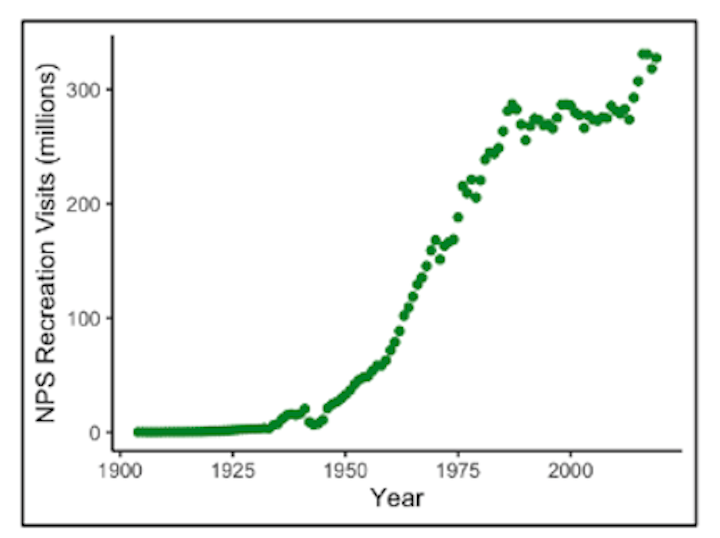
\includegraphics[width=3.79in]{images/problem_statement_figure_1} \caption{Total annual visitors to the National Park Service system, since its inception through 2020. Visitation has been rapidly increasing, particularly within the last decade. (Source: [IRMA](https://irma.nps.gov/Portal/))}\label{fig:fig1}
\end{figure}

\begin{figure}
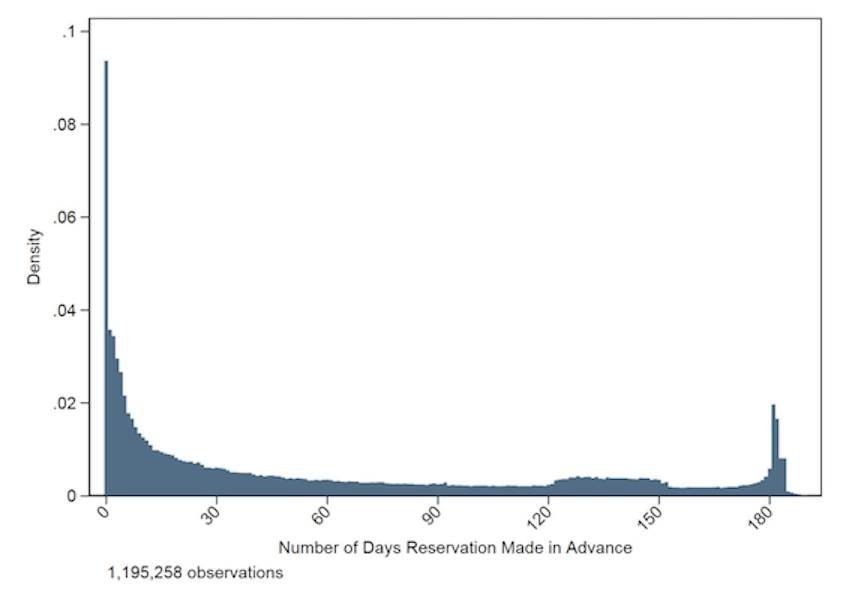
\includegraphics[width=4.32in]{images/problem_statement_figure_2} \caption{Reproduced from @Walls2018. Days in advance that National Park campsite reservations are made from 2014 to 2016. Reservations are made far in advance, but many reservations are canceled at the last minute.}\label{fig:fig2}
\end{figure}

\begin{figure}
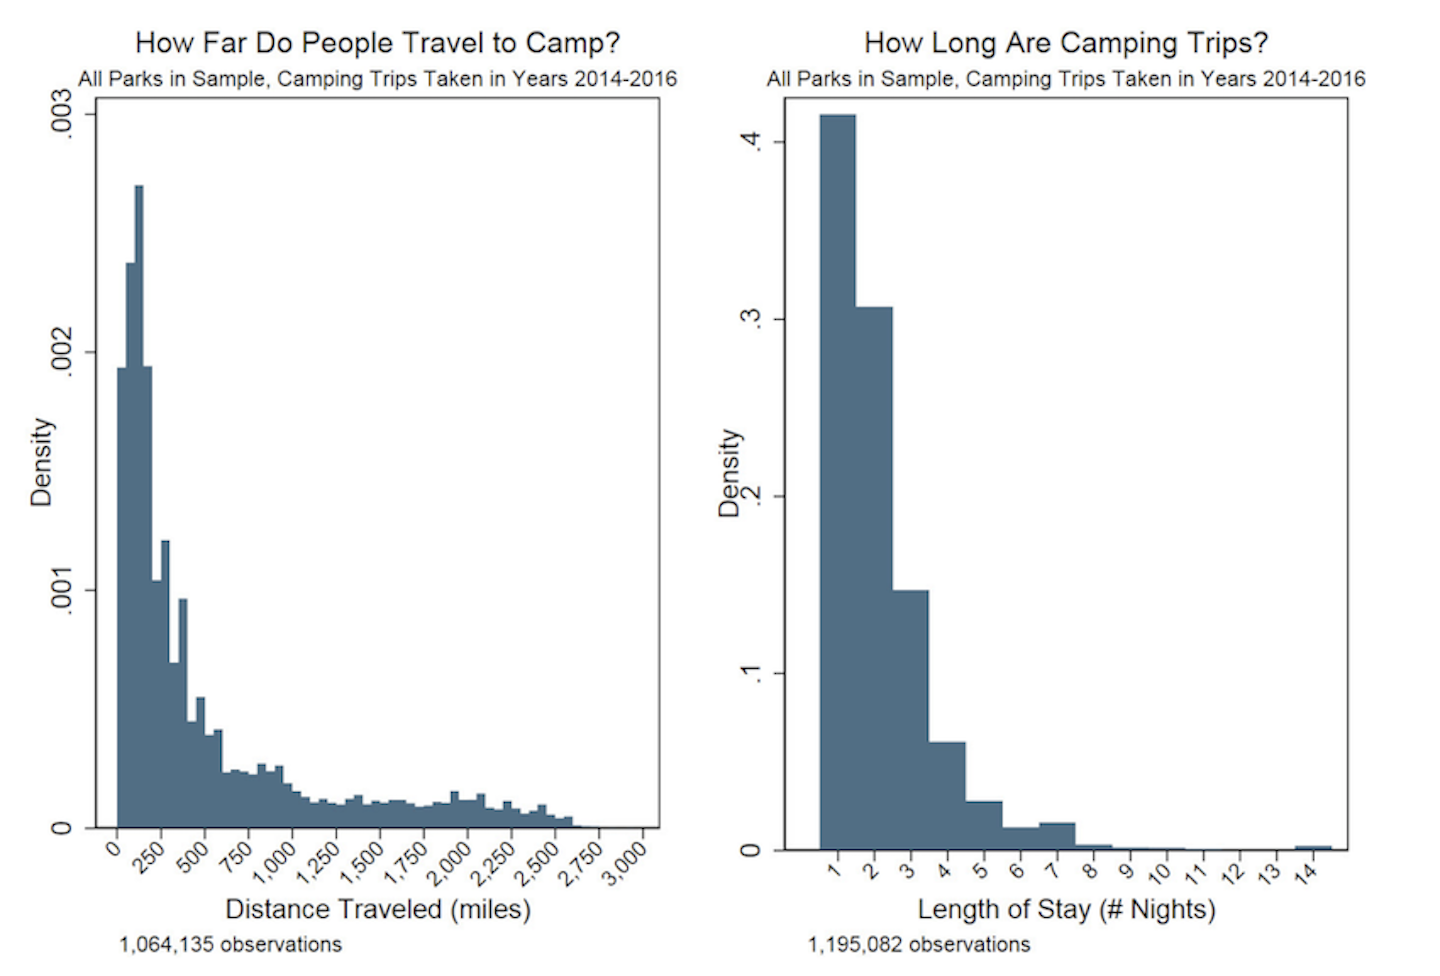
\includegraphics[width=6.4in]{images/problem_statement_figure_3} \caption{Reproduced from @Walls2018. Distance traveled and duration of stay for National Park camping visits from 2014 to 2016. Visitors tend to visit national parks near their homes and stay only two nights, and longer trips are rare.}\label{fig:fig3}
\end{figure}

\begin{figure}
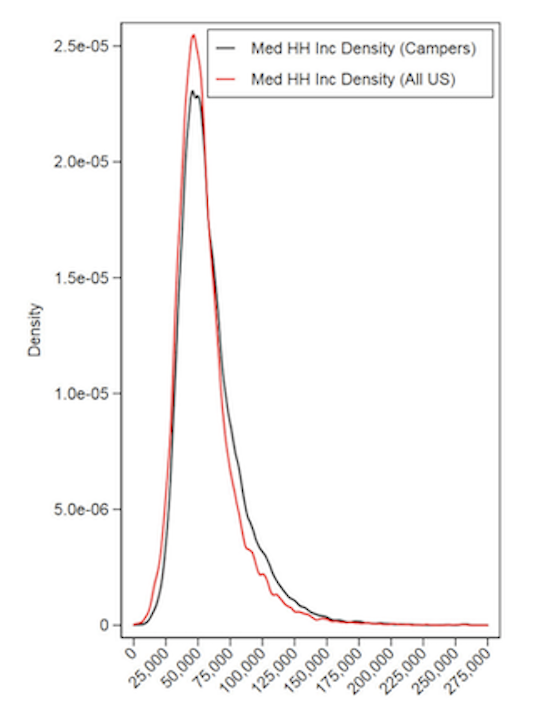
\includegraphics[width=2.95in]{images/problem_statement_figure_4} \caption{Reproduced from @Walls2018. Median household income (by zip code) for National Park campers and for US Population. The black line estimates the distribution of median household (HH) income of campers from 2014 to 2016. The red line estimates the distribution of median household for all zip codes in the U.S. using average median household income from 2014 to 2016 where each zip code is an observation.}\label{fig:fig4}
\end{figure}

\hypertarget{specific-objectives}{%
\chapter{Specific Objectives}\label{specific-objectives}}

Federal lands in the United States provide important recreation opportunities to the public, but there is a \textbf{growing need to understand and mitigate inequities in access to outdoor recreation.} This project addressed this need by creating the \href{https://shinyapps.bren.ucsb.edu/oe_app/}{Outdoor Equity App}, an \textbf{interactive platform} for summarizing and visualizing site-specific patterns and trends in visitation volume, demand, and visitors' location of origin. The platform integrates nationwide \href{https://www.recreation.gov/}{Recreation.gov} reservation data with \href{https://www.census.gov/data.html}{US census data} to:

\begin{itemize}
\tightlist
\item
  Gain insights into \textbf{demand for reservations} across different types of recreation areas.
\item
  Analyze access to federal public lands among \textbf{historically underserved groups} in
  relation to recreation \textbf{site type, cost, location, and demand}.
\item
  Clearly define all variables and values in the \textbf{metadata documentation}.
\item
  Allow users to \textbf{download a subset of the combined data} for further analysis.
\end{itemize}

\hypertarget{summary-of-solution-design}{%
\chapter{Summary of Solution Design}\label{summary-of-solution-design}}

\hypertarget{glossary-and-definitions}{%
\section{Glossary and Definitions}\label{glossary-and-definitions}}

Throughout this document we define ``reservable sites'' as traditional campgrounds, single remote campsites, overnight boat-in sites or mooring, equestrian sites, cabins, and other shelters listed in the \href{https://ridb.recreation.gov/}{RIDB data}.

A full glossary can be found in the \protect\hyperlink{glossary-table}{Appendix Section}.

\hypertarget{access-clean-and-wrangle-data}{%
\section{Access, Clean, and Wrangle Data}\label{access-clean-and-wrangle-data}}

\href{https://ridb.recreation.gov/}{RIDB data} and \href{https://www.census.gov/programs-surveys/acs/data.html}{US Census American Communities Survey (ACS) data} are freely available online to the public. We accessed, cleaned, and wrangled all data outside of the \href{https://shinyapps.bren.ucsb.edu/oe_app/}{Outdoor Equity App} using the \texttt{data\_wrangle\_and\_clean.Rmd} document and 18 custom-made functions (Appendix Table \ref{tab:func-table1}). We downloaded RIDB data in CSV format from Recreation.gov and ACS data through API using the R package \texttt{tidycensus} \citep{R-tidycensus}. We first subsetted RIDB and ACS datasets to include only the variables relevant to our objectives. We then normalized, aggregated, and calculated variables as necessary. Once both datasets are cleaned and wrangled, we joined them using ZIP codes as the key (common value in both datasets). Finally we wrangled the joined RIDB and ACS dataset to ready them for creating data relationship plots.

See the \protect\hyperlink{functions-table}{Appendix Section} for a full table of all functions.

\hypertarget{analysis-and-visualizations}{%
\section{Analysis and Visualizations}\label{analysis-and-visualizations}}

The \href{https://shinyapps.bren.ucsb.edu/oe_app/}{Outdoor Equity App} features interactive maps and plots. Users of this app can select a single reservable site to create custom plots that show a data summary of a single variable or a data relationship between two variables. Visualizations of multiple reservable sites appear as separate plots. Users can also select a single site to create a visitorshed map for the full United States and for the state in which the site is located.

\hypertarget{outdoor-equity-app}{%
\section{Outdoor Equity App}\label{outdoor-equity-app}}

The app has a navigation bar with four tabs: About, Analysis, Metadata and Data Download. Nested under the Analysis tab are the subtabs of Data Summary, Data Relationship, and Visitorshed Maps. The app opens automatically to the About tab.

\begin{figure}
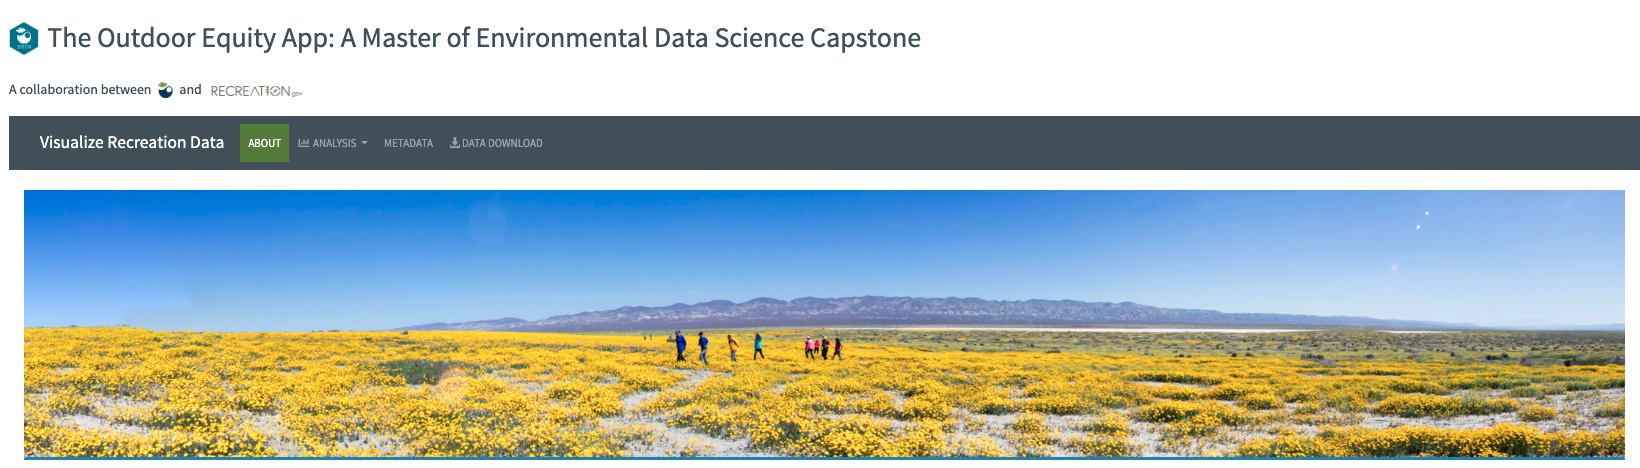
\includegraphics[width=5.96in]{images/screenshot_about} \caption{Screenshot of the About page of the Outdoor Equity App}\label{fig:app-screenshot1}
\end{figure}

\begin{figure}
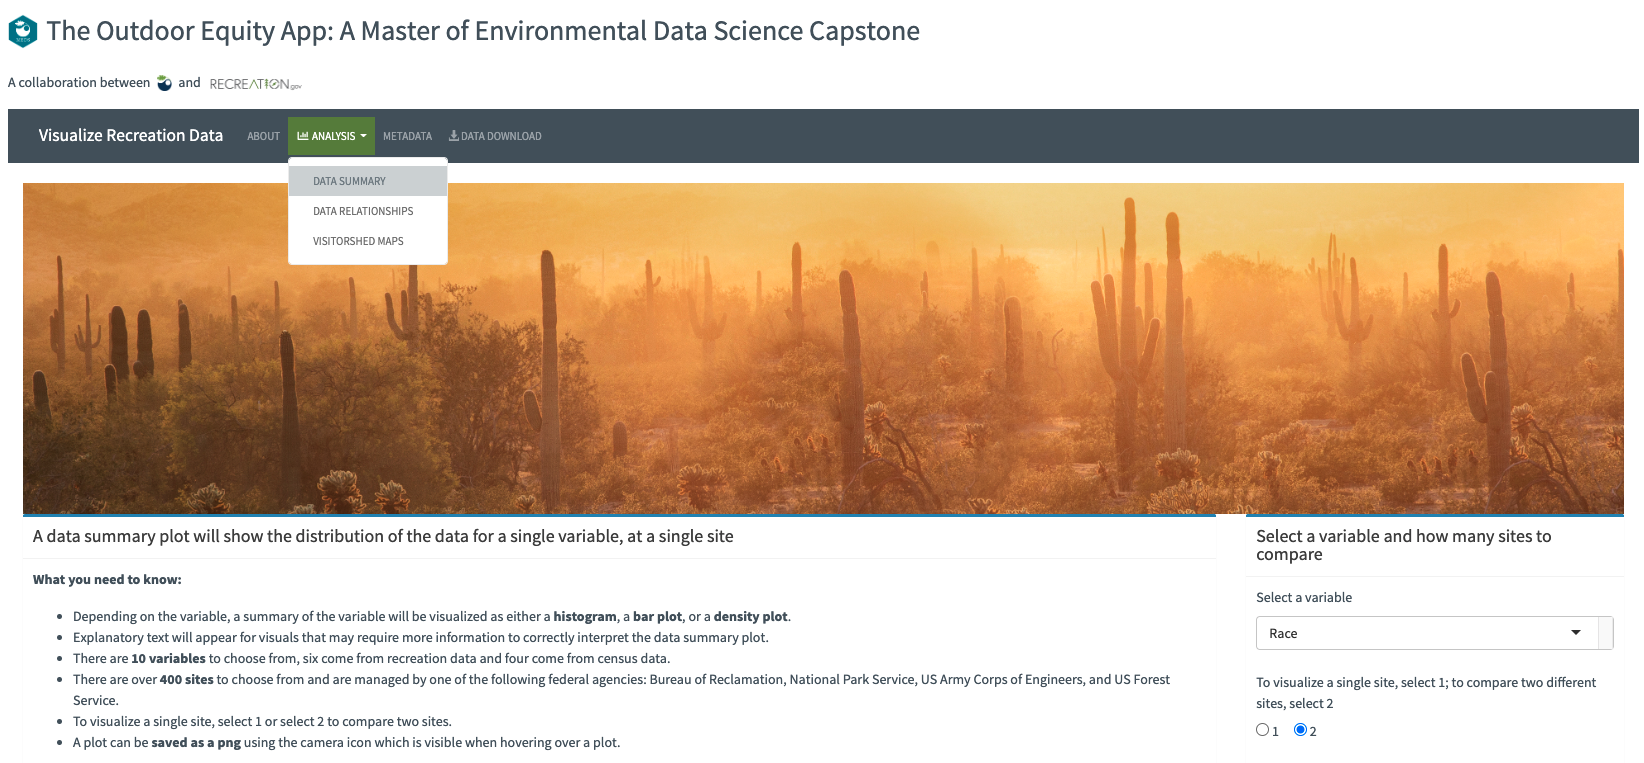
\includegraphics[width=5.98in]{images/screenshot_data-summary} \caption{Screenshot of the Analysis page of the Outdoor Equity App}\label{fig:app-screenshot2}
\end{figure}

\begin{figure}
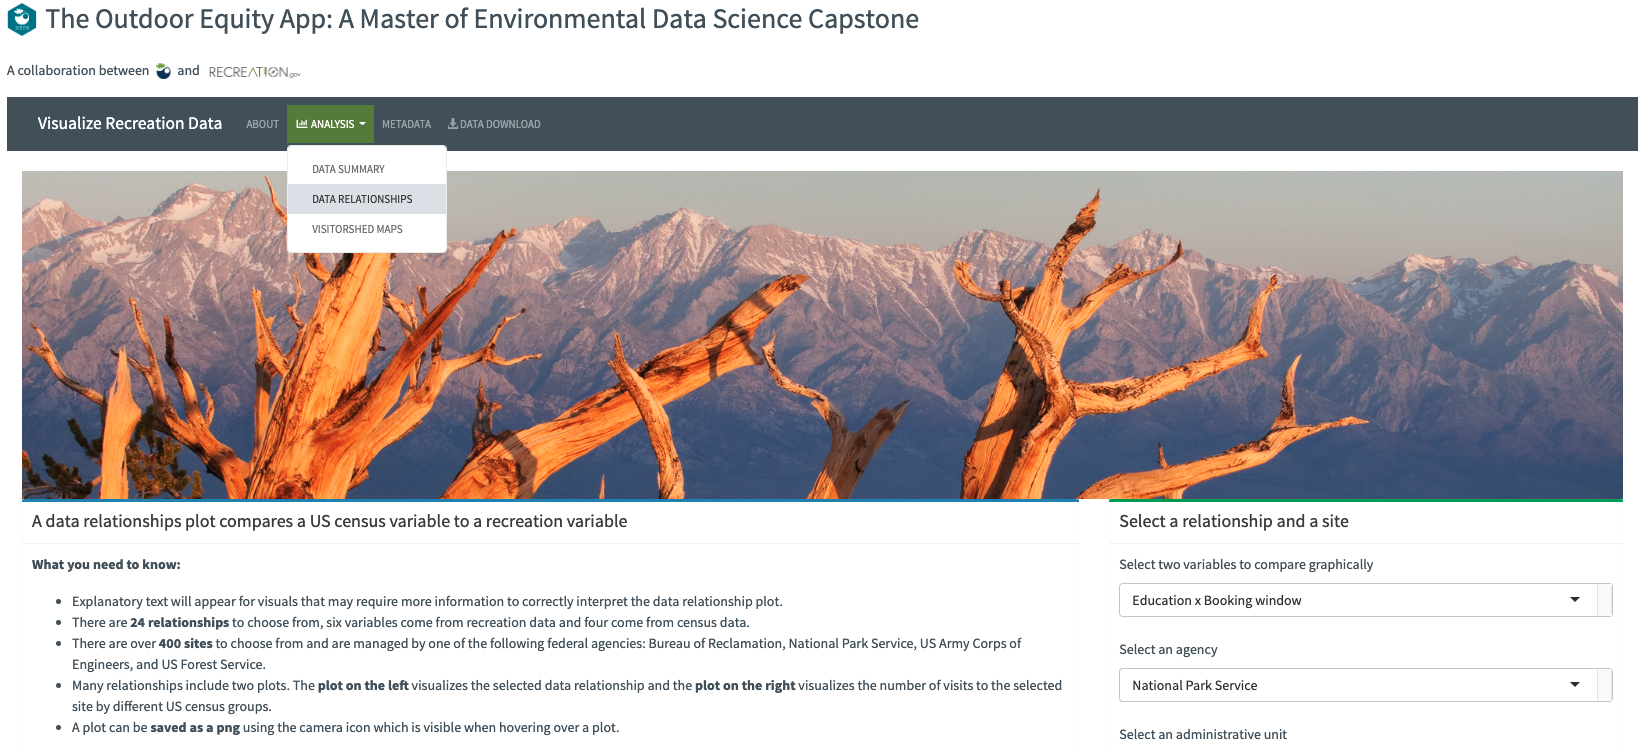
\includegraphics[width=5.96in]{images/screenshot_data-relationship} \caption{Screenshot of the Analysis page of the Outdoor Equity App}\label{fig:app-screenshot3}
\end{figure}

\begin{figure}
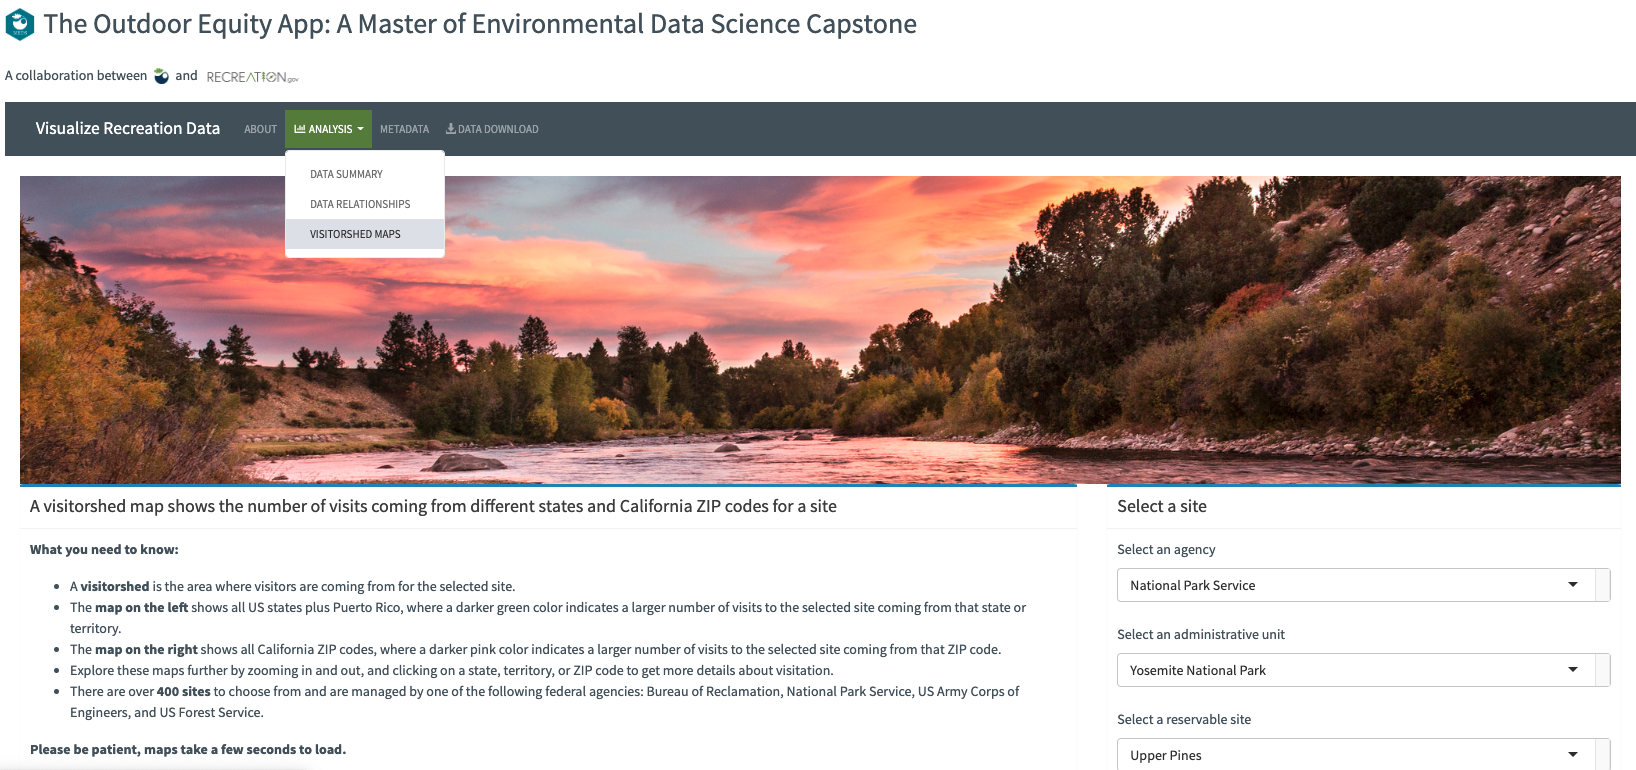
\includegraphics[width=5.95in]{images/screenshot_visitorshed} \caption{Screenshot of the Analysis page of the Outdoor Equity App}\label{fig:app-screenshot4}
\end{figure}

\begin{figure}
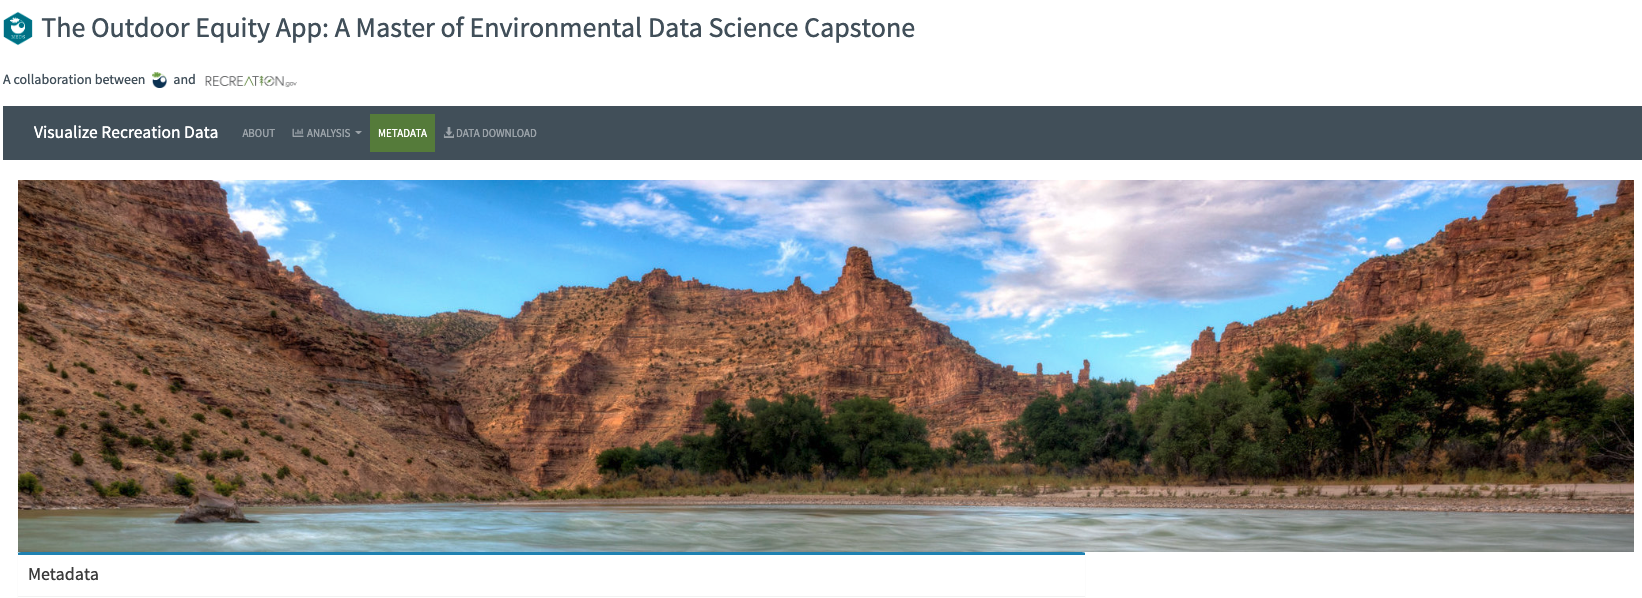
\includegraphics[width=5.97in]{images/screenshot_metadata} \caption{Screenshot of the Metadata page of the Outdoor Equity App}\label{fig:app-screenshot5}
\end{figure}

\begin{figure}
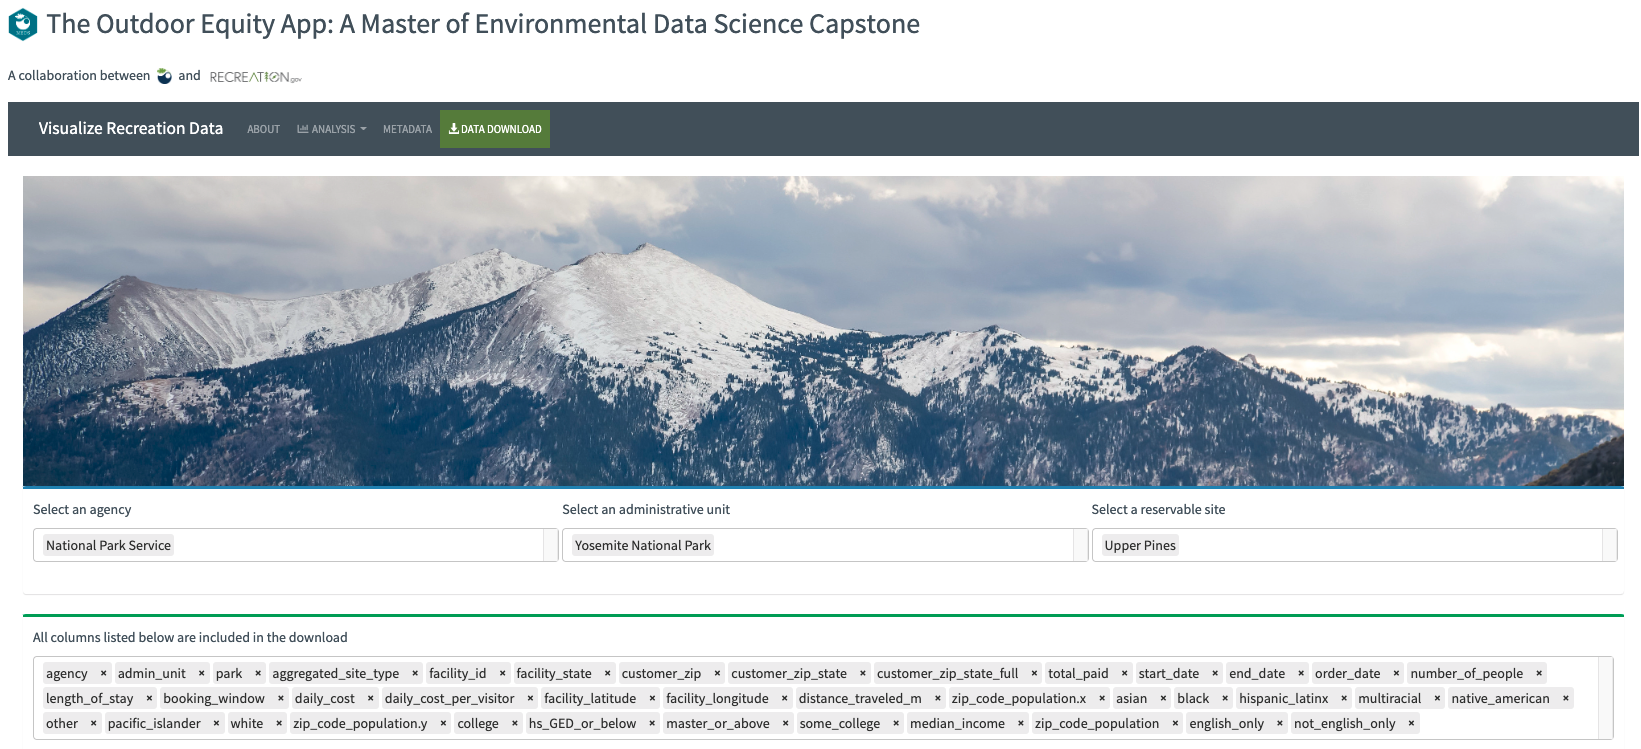
\includegraphics[width=5.97in]{images/screenshot_data-download} \caption{Screenshot of the Metadata page of the Outdoor Equity App}\label{fig:app-screenshot6}
\end{figure}

\hypertarget{user-guide-and-technical-documentation}{%
\section{User Guide and Technical Documentation}\label{user-guide-and-technical-documentation}}

The \href{https://shinyapps.bren.ucsb.edu/oe_app/}{Outdoor Equity App} includes a user guide and metadata information. The user guide section includes a quick overview of the app and helper text on how to start creating visuals.

This technical documentation is created with the \texttt{bookdown} package \citep{R-bookdown} and is linked in the About tab of the Outdoor Equity App. Metadata for all variables used within the app are also available on the app Metadata tab and in the \protect\hyperlink{products-and-deliverables}{Products and Deliverables Section} of this document.

\hypertarget{products-and-deliverables}{%
\chapter{Products and Deliverables}\label{products-and-deliverables}}

\hypertarget{r-shiny-app}{%
\section{R Shiny App}\label{r-shiny-app}}

The \href{https://shinyapps.bren.ucsb.edu/oe_app/}{Outdoor Equity App} was built using the \texttt{shiny} package \citep{R-shiny} and has the following functionality:

\begin{itemize}
\tightlist
\item
  Visualize statistical distributions of \href{https://ridb.recreation.gov/download}{RIDB} and \href{https://www.census.gov/programs-surveys/acs/data.html}{US Census American Community Survey (ACS)} variables
\item
  Visualize relationships between RIDB and ACS variables
\item
  Download visualizations as PNG images
\item
  View visitorshed maps of reservable sites both nationally and within the state where the campsite is located
\item
  Download customized subsets of the data
\end{itemize}

\hypertarget{metadata}{%
\section{Metadata}\label{metadata}}

A condensed list of all metadata can be found in the \protect\hyperlink{metadata-table}{Appendix Section}. A full list of all metadata can be found in the \href{https://shinyapps.bren.ucsb.edu/oe_app/}{Outdoor Equity App} on the Metadata tab.

\hypertarget{packages-and-versions-used}{%
\section{Packages and Versions Used}\label{packages-and-versions-used}}

See the \protect\hyperlink{packages-table}{Appendix Section} for a full list of packages used.

\hypertarget{summary-of-testing}{%
\chapter{Summary of Testing}\label{summary-of-testing}}

\hypertarget{data-integrity}{%
\section{Data Integrity}\label{data-integrity}}

We screened the data for outliers by summarizing and visualizing the raw data, and assessed whether those outliers need to be removed. We consulted other researchers who are familiar with the RIDB datasets to confirm outliers or other anomalies in the data.

Additionally, we documented the percent loss from data wrangling to ensure that our cleaning and wrangling of the data were reasonable.

\hypertarget{code-review}{%
\section{Code Review}\label{code-review}}

We conducted code reviews within the team, and with faculty or external advisers. We reviewed specific code chunks and scripts related to the Outdoor Equity App.

We separated our workflows so that one person created scripts, and the other reviewed them. We did this to maintain some objectivity when evaluating if our datasets were aggregating correctly. We also had a separate workflow for metadata, where one person created and wrote metadata, and the other reviewed it. This confirmed that the data matches how it is being described in the metadata. This confirmation is important as we want our client to be able to scale our product and workflows for future use.

\hypertarget{product-testing}{%
\section{Product Testing}\label{product-testing}}

We used three packages to test our R Shiny app. We used \texttt{shinytest} \citep{R-shinytest} to ensure our app is visualized the way we expect it to using the package's snapshot-based testing strategy. We used \texttt{shinyloadtest} \citep{R-shinyloadtest} to test the server hosting the R Shiny App to ensure that it responds in a reasonable amount of time based on the inputs a user provides. Similarly, we utilized the \texttt{tictoc} \citep{R-tictoc} package during our data wrangling and cleaning, and when we initially created our plots, graphs, and maps to estimate an informed guess of how long it may take the app to run our scripts. Lastly, we used the \texttt{reactlog} \citep{R-reactlog} package's diagnostic tool which creates a reactive visualizer for the app to make sure that reactive elements are working the way we expected them to. It is important to note that this diagnostic tool was not useful as our app functionality increased, as the reactive visualizer became impossible to read. There may be other options within \texttt{reactlog} to use the reactive visualizer in a different way, but we did not have enough time to research this.

We added temporary print statements to all functions in the app to ensure that the functions were working correctly were are outputting what we expect. We removed print statements from functions that were functioning with zero errors. We did this because print statements can take a long time to run and should not be left in functions or in the app permanently.

Additionally, we held multiple meetings with the Recreation One Stop team to obtain real-time and focused feedback to improve user design and experience.

\hypertarget{next-steps-for-testing}{%
\subsection{Next steps for testing}\label{next-steps-for-testing}}

Due to time constraints, we were not able to implement all testing methods we wanted. We recommend the following testing strategies to make the app more robust and for smoother functionality.

\begin{itemize}
\tightlist
\item
  Use the R package \texttt{testthat} \citep{R-testthat} to conduct unit tests on the scripts used to create Tidy datasets and for subsetted datasets for visualization. This type of testing may be important to avoid silent failures and to ensure that the datasets are aggregating correctly.
\item
  Use \href{https://github.com/marmelab/gremlins.js}{\texttt{gremlin.js}}), a JavaScript library used for ``Monkey testing'' to test the behavior of the R Shiny App. This package is compatible with \texttt{shiny} \citep{R-shiny} and does not require any external installation. See \href{https://engineering-shiny.org/build-yourself-safety-net.html}{Chapter 11 in Engineering Production-Grade Shiny Apps} for more guidance. ``Monkey testing'' is a type of testing where random, automated tests provide random inputs and then checks the behavior of the app (i.e.~if the system or application crashes). We were able to find some finicky bugs through our own testing of random inputs, but ``Monkey testing'' is the formal process of testing app behavior.
\item
  Employ user testing with federal public land managers, researchers, and those who are not familiar with RIDB data to further enhance the user experience and design.
\end{itemize}

\hypertarget{user-documentation}{%
\chapter{User Documentation}\label{user-documentation}}

\hypertarget{purpose-of-the-outdoor-equity-app}{%
\section{Purpose of the Outdoor Equity App}\label{purpose-of-the-outdoor-equity-app}}

The \href{https://shinyapps.bren.ucsb.edu/oe_app/}{Outdoor Equity App} provides users with tools to explore trends at different overnight reservable sites to analyze access to these sites. The intended audience is federal public land managers and researchers as well as nonprofit organizations and recreation users.

The \href{https://ridb.recreation.gov/landing}{Recreation Information Database (RIDB) data} are comprehensive when it comes to information regarding the site and reservation, but do not include information about the visitor outside of their home ZIP code. \href{https://www.census.gov/programs-surveys/acs/data.html}{US Census American Community Survey (ACS) data} is used to approximate socioeconomic demographics by joining information about the visitors' home ZIP code to the RIDB data.

\hypertarget{how-to-use-the-outdoor-equity-app}{%
\section{How to Use the Outdoor Equity App}\label{how-to-use-the-outdoor-equity-app}}

\hypertarget{about-the-app}{%
\subsection{About the App}\label{about-the-app}}

The About tab of the \href{https://shinyapps.bren.ucsb.edu/oe_app/}{Outdoor Equity App} includes background information about what the App is, why outdoor recreation is important, the App creators, and what data is used in the App. These sections are similar to the \protect\hyperlink{about}{About Section} of this technical documentation. The About tab also includes example questions that a user might explore through the different parts of the Analysis tab.

The Analysis tab of the App consists of three parts Data Summary, Data Relationship and Visitorshed Maps. Each of these pages includes a brief explanatory section of how to interpret the plot or graph, a section to subset the data to the desired campsite, and the plot or map outputs.

The Metadata tab of the App includes metadata for all variables in the combined RIDB and ACS dataset. This section mirrors the Metadata section in the \protect\hyperlink{products-and-deliverables}{Products and Deliverables Section} of this document.

The Data Download section of the App allows a user to download a subset of data include as many or as few campsites and variables as they require for further analysis or use.

\hypertarget{how-to-maintain-the-outdoor-equity-app}{%
\section{How to Maintain the Outdoor Equity App}\label{how-to-maintain-the-outdoor-equity-app}}

\hypertarget{repository-directory-structure}{%
\subsection{Repository Directory Structure}\label{repository-directory-structure}}

Our code is version controlled in a \href{https://github.com/outdoor-equity/outdoor-equity}{GitHub repository}. This includes the data cleaning, wrangling, and analysis, creation of plots and maps, and structure of the shiny app. An overview of the directory structure can be found in the \protect\hyperlink{repository-directory-structure-1}{Appendix Section}.

\hypertarget{data-preparation-methods}{%
\subsection{Data Preparation Methods}\label{data-preparation-methods}}

\hypertarget{ridb-data}{%
\subsubsection{RIDB Data}\label{ridb-data}}

\href{https://ridb.recreation.gov/landing}{RIDB data} data are available through direct download as CSV files or via the API as JSON files via Recreation.gov. API access requires creating a Recreation.gov account and requesting second tier API access via the Recreation.gov website's \href{https://recreationonestopprod.servicenowservices.com/external?id=external_contact_us}{Contact Us} page. CSV files are readily available for download via the \href{https://ridb.recreation.gov/download}{Recreation.gov website}. Data are collected each time a visitor makes a reservation through Recreation.gov. Data packages are posted annually in the spring by Recreation One Stop (R1S) and contain the previous fiscal year's reservations (ex: the 2018 package includes 2018-10-01 through 2018-09-30). Data packages are available for download from 2006 to present. Each annual data package file contains a range between 2 million and 5 million observations (or reservations) and includes variables in character, numeric, and date/time formats about each reservation. A shift in the data collection and storage processes occurred in 2019, changing what variables are available and how they are labeled. Currently, the Outdoor Equity App contains only data for reservable sites in California and reservations for fiscal year 2018 due to time limitations of this project. To see more about expanding the App temporally and spatially see the \protect\hyperlink{how-to-expand-the-outdoor-equity-app}{How to Expand the Outdoor Equity App Section}.

We created a reproducible workflow for cleaning and wrangling data, which is employed in the \texttt{data\_wrangle\_and\_clean.Rmd} document that sources custom functions to prepare RIDB data for joining with ACS data. All custom functions are listed in the \protect\hyperlink{access-clean-and-wrangle-data}{Access, Clean, and Wrangle Data Section} of this document. These functions rely heavily on functions from the \texttt{tidyverse} collection of packages \citep{R-tidyverse}.

First, we use the \texttt{function\_ridb\_subset-pre2018.R} to subset the RIDB data, filtering only reservations within the selected state that are listed as ``Overnight'' reservations within the \texttt{use\_type} variable. For the 2018 California dataset this results in a starting ``raw'' data frame with 521,682 reservations

\begin{Shaded}
\begin{Highlighting}[]
\CommentTok{\# filter for state}
\FunctionTok{filter}\NormalTok{(facility\_state }\SpecialCharTok{==}\NormalTok{ state\_abbrev) }\SpecialCharTok{\%\textgreater{}\%}
  \CommentTok{\# filter for use type}
  \FunctionTok{filter}\NormalTok{(use\_type }\SpecialCharTok{==} \StringTok{"Overnight"}\NormalTok{)}
\end{Highlighting}
\end{Shaded}

We then select only the necessary variables, including information about the site (agency, park or forest name, site name, site type, and site location) and information about the reservation (home ZIP come, total paid, visit start and end dates, visit order date, and number of people in party).

\begin{Shaded}
\begin{Highlighting}[]
\CommentTok{\# select variables}
\FunctionTok{select}\NormalTok{(}\FunctionTok{c}\NormalTok{(}\StringTok{"agency"}\NormalTok{, }\StringTok{"parent\_location"}\NormalTok{, }\StringTok{"region\_description"}\NormalTok{, }
         \StringTok{"park"}\NormalTok{, }\StringTok{"site\_type"}\NormalTok{, }\StringTok{"facility\_id"}\NormalTok{, }\StringTok{"facility\_state"}\NormalTok{, }
         \StringTok{"facility\_longitude"}\NormalTok{, }\StringTok{"facility\_latitude"}\NormalTok{, }
         \StringTok{"customer\_zip"}\NormalTok{, }\StringTok{"total\_paid"}\NormalTok{, }\StringTok{"start\_date"}\NormalTok{,}
         \StringTok{"end\_date"}\NormalTok{, }\StringTok{"order\_date"}\NormalTok{, }\StringTok{"number\_of\_people"}\NormalTok{)) }\SpecialCharTok{\%\textgreater{}\%}
  \FunctionTok{mutate}\NormalTok{(}\AttributeTok{site\_type =} \FunctionTok{tolower}\NormalTok{(site\_type)) }\SpecialCharTok{\%\textgreater{}\%}
  \FunctionTok{filter}\NormalTok{(}\SpecialCharTok{!}\NormalTok{site\_type }\SpecialCharTok{\%in\%} \FunctionTok{c}\NormalTok{(}\StringTok{"historic tour"}\NormalTok{, }\StringTok{"hiking zone"}\NormalTok{, }
                           \StringTok{"group picnic area"}\NormalTok{, }\StringTok{"cave tour"}\NormalTok{,}
                           \StringTok{"management"}\NormalTok{, }\StringTok{"picnic"}\NormalTok{, }
                           \StringTok{"entry point"}\NormalTok{, }\StringTok{"trailhead"}\NormalTok{))}
\end{Highlighting}
\end{Shaded}

Next we normalize the customer ZIP code values. This includes filtering for only US ZIP codes and shortening all 9 digit ZIP codes to include only the first 5 digits.

\begin{Shaded}
\begin{Highlighting}[]
\CommentTok{\# filter out invalid ZIP codes}
\FunctionTok{filter}\NormalTok{(}\FunctionTok{str\_detect}\NormalTok{(}\AttributeTok{string =}\NormalTok{ customer\_zip,}
                  \AttributeTok{pattern =} \StringTok{"\^{}[:digit:]\{5\}(?!.)"}\NormalTok{) }\SpecialCharTok{|}
         \FunctionTok{str\_detect}\NormalTok{(}\AttributeTok{string =}\NormalTok{ customer\_zip,}
                    \AttributeTok{pattern =} \StringTok{"\^{}[:digit:]\{5\}(?={-})"}\NormalTok{)) }\SpecialCharTok{\%\textgreater{}\%}
  \FunctionTok{filter}\NormalTok{(}\SpecialCharTok{!}\NormalTok{customer\_zip }\SpecialCharTok{\%in\%} \FunctionTok{c}\NormalTok{(}\StringTok{"00000"}\NormalTok{, }\StringTok{"99999"}\NormalTok{)) }\SpecialCharTok{\%\textgreater{}\%}
  \FunctionTok{mutate}\NormalTok{(}\AttributeTok{customer\_zip =} \FunctionTok{str\_extract}\NormalTok{(}\AttributeTok{string =}\NormalTok{ customer\_zip,}
                                    \AttributeTok{pattern =} \StringTok{"[:digit:]\{5\}"}\NormalTok{))}
\end{Highlighting}
\end{Shaded}

This function results in the removal of 24,866 reservations (or 4.77\%) from the original ``raw'' dataset that included all reservations for reservable overnight campsites in California.

We created a second custom function \texttt{function\_ridb\_variable\_calculate-pre2018.R} to calculate and manipulate variables of interest. We use start, end, and order dates to calculate the lengths of stay and booking windows (number of days from order to start date) of each reservation. The booking window calculations return a number of results that are negative. This is a known issue that others working with the RIDB data have encountered. This resulted in 4,530 reservations (or 0.87\%) without a valid booking window, which are removed for plots that visualize the booking window variable.

\begin{Shaded}
\begin{Highlighting}[]
\FunctionTok{mutate}\NormalTok{(}\AttributeTok{start\_date =} \FunctionTok{as.Date}\NormalTok{(start\_date),}
       \AttributeTok{end\_date =} \FunctionTok{as.Date}\NormalTok{(end\_date),}
       \AttributeTok{order\_date =} \FunctionTok{as.Date}\NormalTok{(order\_date),}
       \CommentTok{\# calculate new variables}
       \AttributeTok{length\_of\_stay =} \FunctionTok{as.numeric}\NormalTok{(}\FunctionTok{difftime}\NormalTok{(end\_date, start\_date), }
                                   \AttributeTok{units =} \StringTok{"days"}\NormalTok{),}
       \AttributeTok{booking\_window =} \FunctionTok{as.numeric}\NormalTok{(}\FunctionTok{difftime}\NormalTok{(start\_date, order\_date), }
                                   \AttributeTok{units =} \StringTok{"days"}\NormalTok{))}
\end{Highlighting}
\end{Shaded}

We calculate daily cost per reservation by dividing total costs by lengths of stay. We then calculated daily cost per visitor by dividing the daily cost by the number of visitors.

\begin{Shaded}
\begin{Highlighting}[]
\CommentTok{\# calculate new variables}
\FunctionTok{mutate}\NormalTok{(}\AttributeTok{daily\_cost =}\NormalTok{ total\_paid }\SpecialCharTok{/}\NormalTok{ length\_of\_stay,}
       \AttributeTok{daily\_cost\_per\_visitor =}\NormalTok{ daily\_cost }\SpecialCharTok{/}\NormalTok{ number\_of\_people)}
\end{Highlighting}
\end{Shaded}

We aggregate the \texttt{site\_type} variable to create 7 broader site categories.

\begin{Shaded}
\begin{Highlighting}[]
\CommentTok{\# aggregate site type}
\FunctionTok{mutate}\NormalTok{(}\AttributeTok{aggregated\_site\_type =} 
         \FunctionTok{case\_when}\NormalTok{(site\_type }\SpecialCharTok{\%in\%} \FunctionTok{c}\NormalTok{(}\StringTok{"walk to"}\NormalTok{, }\StringTok{"hike to"}\NormalTok{, }
                                    \StringTok{"group hike to"}\NormalTok{, }\StringTok{"group walk to"}
\NormalTok{         ) }\SpecialCharTok{\textasciitilde{}} \StringTok{"remote"}\NormalTok{,}
\NormalTok{         site\_type }\SpecialCharTok{\%in\%} \FunctionTok{c}\NormalTok{(}\StringTok{"cabin nonelectric"}\NormalTok{, }\StringTok{"cabin electric"}\NormalTok{, }
                          \StringTok{"yurt"}\NormalTok{,}\StringTok{"shelter nonelectric"}
\NormalTok{         ) }\SpecialCharTok{\textasciitilde{}} \StringTok{"shelter"}\NormalTok{,}
\NormalTok{         site\_type }\SpecialCharTok{\%in\%} \FunctionTok{c}\NormalTok{(}\StringTok{"boat in"}\NormalTok{, }\StringTok{"anchorage"}\NormalTok{) }\SpecialCharTok{\textasciitilde{}} \StringTok{"water"}\NormalTok{,}
\NormalTok{         site\_type }\SpecialCharTok{\%in\%} \FunctionTok{c}\NormalTok{(}\StringTok{"group equestrian"}\NormalTok{, }
                          \StringTok{"equestrian nonelectric"}
\NormalTok{         ) }\SpecialCharTok{\textasciitilde{}} \StringTok{"equestrian"}\NormalTok{,}
\NormalTok{         site\_type }\SpecialCharTok{\%in\%} \FunctionTok{c}\NormalTok{(}\StringTok{"rv nonelectric"}\NormalTok{, }\StringTok{"rv electric"}\NormalTok{, }
                          \StringTok{"group rv area nonelectric"}
\NormalTok{         ) }\SpecialCharTok{\textasciitilde{}} \StringTok{"rv only"}\NormalTok{,}
\NormalTok{         site\_type }\SpecialCharTok{\%in\%} \FunctionTok{c}\NormalTok{(}\StringTok{"group standard nonelectric"}\NormalTok{, }
                          \StringTok{"standard nonelectric"}\NormalTok{,}
                          \StringTok{"standard electric"}\NormalTok{, }
                          \StringTok{"group standard area nonelectric"}\NormalTok{,}
                          \StringTok{"group standard electric"}
\NormalTok{         ) }\SpecialCharTok{\textasciitilde{}} \StringTok{"rv or tent"}\NormalTok{,}
\NormalTok{         site\_type }\SpecialCharTok{\%in\%} \FunctionTok{c}\NormalTok{(}\StringTok{"tent only nonelectric"}\NormalTok{, }
                          \StringTok{"group tent only area nonelectric"}\NormalTok{,}
                          \StringTok{"tent only electric"}
\NormalTok{         ) }\SpecialCharTok{\textasciitilde{}} \StringTok{"tent only"}\NormalTok{))}
\end{Highlighting}
\end{Shaded}

We create an administrative unit variable by combining the \texttt{parent\_location} and \texttt{region\_description} variables as different federal agencies track the administrative unit information within different variables. Then we update the \texttt{agency}, \texttt{admin\_uni} and \texttt{park} variable character strings using multiple functions from the \texttt{stringr} package \citep{R-stringr}. These updates expand acronyms, remove unnecessary characters (such as ``--'' or location codes), and normalize any discrepencies in characater strings.

\begin{Shaded}
\begin{Highlighting}[]
\FunctionTok{mutate}\NormalTok{(}\AttributeTok{admin\_unit =} 
         \FunctionTok{case\_when}\NormalTok{(agency }\SpecialCharTok{==} \StringTok{"USFS"} \SpecialCharTok{\textasciitilde{}}\NormalTok{ parent\_location,}
\NormalTok{                   agency }\SpecialCharTok{\%in\%} \FunctionTok{c}\NormalTok{(}
                     \StringTok{"NPS"}\NormalTok{, }\StringTok{"BOR"}\NormalTok{, }\StringTok{"USACE"}
\NormalTok{                   ) }\SpecialCharTok{\textasciitilde{}}\NormalTok{ region\_description)) }\SpecialCharTok{\%\textgreater{}\%} 
  \CommentTok{\# edit values}
  \FunctionTok{mutate}\NormalTok{(}
    \CommentTok{\# agency abbreviations to names}
    \AttributeTok{agency =} \FunctionTok{str\_replace}\NormalTok{(}\AttributeTok{string =}\NormalTok{ agency,}
                         \AttributeTok{pattern =} \StringTok{"NPS"}\NormalTok{,}
                         \AttributeTok{replacement =} \StringTok{"National Park Service"}\NormalTok{),}
    \AttributeTok{agency =} \FunctionTok{str\_replace}\NormalTok{(}\AttributeTok{string =}\NormalTok{ agency,}
                         \AttributeTok{pattern =} \StringTok{"USFS"}\NormalTok{, }
                         \AttributeTok{replacement =} \StringTok{"US Forest Service"}\NormalTok{),}
    \AttributeTok{agency =} \FunctionTok{str\_replace}\NormalTok{(}\AttributeTok{string =}\NormalTok{ agency,}
                         \AttributeTok{pattern =} \StringTok{"USACE"}\NormalTok{,}
                         \AttributeTok{replacement =} \StringTok{"US Army Corps of Engineers"}\NormalTok{),}
    \AttributeTok{agency =} \FunctionTok{str\_replace}\NormalTok{(}\AttributeTok{string =}\NormalTok{ agency,}
                         \AttributeTok{pattern =} \StringTok{"BOR"}\NormalTok{,}
                         \AttributeTok{replacement =} \StringTok{"Bureau of Reclamation"}\NormalTok{),}
    \CommentTok{\# update admin\_unit values (generic)}
    \AttributeTok{admin\_unit =} \FunctionTok{str\_replace}\NormalTok{(}\AttributeTok{string =}\NormalTok{ admin\_unit,}
                             \AttributeTok{pattern =} \FunctionTok{paste}\NormalTok{(}\FunctionTok{c}\NormalTok{(}\StringTok{"NF {-} FS"}\NormalTok{, }\StringTok{"NF {-}FS"}\NormalTok{, }
                                               \StringTok{"NF{-} FS"}\NormalTok{, }\StringTok{"NF{-}FS"}\NormalTok{, }
                                               \StringTok{"{-}FS"}\NormalTok{, }\StringTok{" {-} FS"}\NormalTok{), }
                                             \AttributeTok{collapse =} \StringTok{"|"}\NormalTok{),}
                             \AttributeTok{replacement =} \StringTok{"National Forest"}\NormalTok{),}
    \AttributeTok{admin\_unit =} \FunctionTok{str\_to\_title}\NormalTok{(admin\_unit),}
    \AttributeTok{admin\_unit =} \FunctionTok{str\_replace}\NormalTok{(}\AttributeTok{string =}\NormalTok{ admin\_unit,}
                             \AttributeTok{pattern =} \StringTok{"And"}\NormalTok{,}
                             \AttributeTok{replacement =} \StringTok{"\&"}\NormalTok{),}
    \CommentTok{\# update park values (generic)}
    \AttributeTok{park =} \FunctionTok{str\_remove}\NormalTok{(}\AttributeTok{string =}\NormalTok{ park,}
                      \AttributeTok{pattern =} \FunctionTok{paste}\NormalTok{(}\FunctionTok{c}\NormalTok{(}\StringTok{"}\SpecialCharTok{\textbackslash{}\textbackslash{}}\StringTok{(.*"}\NormalTok{, }\StringTok{" }\SpecialCharTok{\textbackslash{}\textbackslash{}}\StringTok{(.*"}\NormalTok{,}
                                        \StringTok{"{-}{-}{-}.*"}\NormalTok{, }\StringTok{" {-}{-}{-}.*"}\NormalTok{,}
                                        \StringTok{",.*"}\NormalTok{), }
                                      \AttributeTok{collapse =} \StringTok{"|"}\NormalTok{)),}
    \AttributeTok{park =} \FunctionTok{str\_to\_title}\NormalTok{(park),}
    \AttributeTok{park =} \FunctionTok{str\_replace}\NormalTok{(}\AttributeTok{string =}\NormalTok{ park,}
                       \AttributeTok{pattern =} \StringTok{"Cg"}\NormalTok{,}
                       \AttributeTok{replacement =} \StringTok{"Campground"}\NormalTok{),}
    \AttributeTok{park =} \FunctionTok{str\_replace}\NormalTok{(}\AttributeTok{string =}\NormalTok{ park,}
                       \AttributeTok{pattern =} \StringTok{"Nhp"}\NormalTok{,}
                       \AttributeTok{replacement =} \StringTok{"National Historic Park"}\NormalTok{),}
    \AttributeTok{park =} \FunctionTok{str\_replace}\NormalTok{(}\AttributeTok{string =}\NormalTok{ park,}
                       \AttributeTok{pattern =} \StringTok{"@"}\NormalTok{,}
                       \AttributeTok{replacement =} \StringTok{"At"}\NormalTok{),}
    \AttributeTok{park =} \FunctionTok{str\_replace}\NormalTok{(}\AttributeTok{string =}\NormalTok{ park,}
                       \AttributeTok{pattern =} \StringTok{"\&"}\NormalTok{,}
                       \AttributeTok{replacement =} \StringTok{"And"}\NormalTok{),}
    \AttributeTok{park =} \FunctionTok{str\_replace}\NormalTok{(}\AttributeTok{string =}\NormalTok{ park,}
                       \AttributeTok{pattern =} \FunctionTok{paste}\NormalTok{(}\FunctionTok{c}\NormalTok{(}\StringTok{"/"}\NormalTok{, }\StringTok{" / "}\NormalTok{), }\AttributeTok{collapse =} \StringTok{"|"}\NormalTok{),}
                       \AttributeTok{replacement =} \StringTok{" "}\NormalTok{),}
    \AttributeTok{park =} \FunctionTok{str\_remove\_all}\NormalTok{(}\AttributeTok{string =}\NormalTok{ park,}
                          \AttributeTok{pattern =} \StringTok{" }\SpecialCharTok{\textbackslash{}\textbackslash{}}\StringTok{d.*"}\NormalTok{),}
    \CommentTok{\# update park values (CA specific)}
    \AttributeTok{park =} \FunctionTok{str\_remove}\NormalTok{(}\AttributeTok{string =}\NormalTok{ park,}
                      \AttributeTok{pattern =} \FunctionTok{paste}\NormalTok{(}\FunctionTok{c}\NormalTok{(}\StringTok{" {-} Angeles Nf"}\NormalTok{, }\StringTok{" {-}Hwy"}\NormalTok{), }
                                      \AttributeTok{collapse =} \StringTok{"|"}\NormalTok{)),}
    \AttributeTok{park =} \FunctionTok{str\_replace}\NormalTok{(}\AttributeTok{string =}\NormalTok{ park,}
                       \AttributeTok{pattern =} \StringTok{"Tunnel Mills Il"}\NormalTok{,}
                       \AttributeTok{replacement =} \StringTok{"Tunnel Mills"}\NormalTok{))}
\end{Highlighting}
\end{Shaded}

We calculate distance traveled by measuring the distance from the latitude and longitude coordinate facility locations to the centroid of the home ZIP code. Here we utilize both the \texttt{tidycensus} package \citep{R-tidycensus} and the \texttt{sf} package \citep{R-sf}.

\begin{Shaded}
\begin{Highlighting}[]
\CommentTok{\# bootstrap geometries and reproject to NAD 83}
\NormalTok{df\_geometries }\OtherTok{\textless{}{-}}\NormalTok{ df }\SpecialCharTok{\%\textgreater{}\%} 
  \FunctionTok{st\_as\_sf}\NormalTok{(}\AttributeTok{coords =} \FunctionTok{c}\NormalTok{(}\StringTok{"facility\_longitude"}\NormalTok{, }\StringTok{"facility\_latitude"}\NormalTok{),}
           \AttributeTok{crs =} \DecValTok{4326}\NormalTok{) }\SpecialCharTok{\%\textgreater{}\%} 
  \FunctionTok{st\_transform}\NormalTok{(}\AttributeTok{crs =} \DecValTok{4269}\NormalTok{) }\CommentTok{\# using NAD83 because measured in meters}

\CommentTok{\# get centroid of geometries for all US ZIP codes }
\NormalTok{df\_zip\_centroids\_us }\OtherTok{\textless{}{-}} 
  \FunctionTok{get\_acs}\NormalTok{(}\AttributeTok{geography =} \StringTok{"zcta"}\NormalTok{, }\AttributeTok{year =} \DecValTok{2018}\NormalTok{, }
          \AttributeTok{geometry =} \ConstantTok{TRUE}\NormalTok{, }
          \AttributeTok{summary\_var =} \StringTok{"B01001\_001"}\NormalTok{,}
          \AttributeTok{survey =} \StringTok{"acs5"}\NormalTok{,}
          \AttributeTok{variables =} \FunctionTok{c}\NormalTok{(}\AttributeTok{male =} \StringTok{"B01001\_002"}\NormalTok{)) }\SpecialCharTok{\%\textgreater{}\%} 
  \FunctionTok{select}\NormalTok{(NAME, geometry) }\SpecialCharTok{\%\textgreater{}\%} 
  \FunctionTok{mutate}\NormalTok{(}\AttributeTok{zip\_code =} \FunctionTok{str\_sub}\NormalTok{(NAME, }\AttributeTok{start =} \SpecialCharTok{{-}}\DecValTok{5}\NormalTok{, }\AttributeTok{end =} \SpecialCharTok{{-}}\DecValTok{1}\NormalTok{)) }\SpecialCharTok{\%\textgreater{}\%} 
  \FunctionTok{select}\NormalTok{(zip\_code, geometry) }\SpecialCharTok{\%\textgreater{}\%} 
  \FunctionTok{st\_centroid}\NormalTok{()}

\CommentTok{\# join data and calculate \textasciigrave{}distance\_traveled\textasciigrave{} variable}
\NormalTok{df\_joined\_geometries }\OtherTok{\textless{}{-}} 
  \FunctionTok{left\_join}\NormalTok{(}\AttributeTok{x =}\NormalTok{ df\_geometries }\SpecialCharTok{\%\textgreater{}\%} \FunctionTok{as.data.frame}\NormalTok{(),}
            \AttributeTok{y =}\NormalTok{ df\_zip\_centroids\_us }\SpecialCharTok{\%\textgreater{}\%} \FunctionTok{as.data.frame}\NormalTok{(), }
            \AttributeTok{by =} \FunctionTok{c}\NormalTok{(}\StringTok{"customer\_zip"} \OtherTok{=} \StringTok{"zip\_code"}\NormalTok{)) }\SpecialCharTok{\%\textgreater{}\%}
  \FunctionTok{st\_sf}\NormalTok{(}\AttributeTok{sf\_column\_name =} \StringTok{\textquotesingle{}geometry.x\textquotesingle{}}\NormalTok{) }\SpecialCharTok{\%\textgreater{}\%} 
  \FunctionTok{mutate}\NormalTok{(}\AttributeTok{distance\_traveled\_m =} \FunctionTok{st\_distance}\NormalTok{(}\AttributeTok{x =}\NormalTok{ geometry.x, }
                                           \AttributeTok{y =}\NormalTok{ geometry.y,}
                                           \AttributeTok{by\_element =} \ConstantTok{TRUE}\NormalTok{),}
         \AttributeTok{distance\_traveled\_m =} \FunctionTok{as.numeric}\NormalTok{(distance\_traveled\_m)) }
\end{Highlighting}
\end{Shaded}

And finally, we add a variable indicating in which state or territory each customer zip code is located. This portion of the code utilizes the \texttt{zipcodeR} package \citep{R-zipcodeR}.

\begin{Shaded}
\begin{Highlighting}[]
\CommentTok{\# create df of fips and full state names}
\NormalTok{fips\_list }\OtherTok{\textless{}{-}} \FunctionTok{c}\NormalTok{(}
  \StringTok{"01"}\NormalTok{, }\StringTok{"02"}\NormalTok{, }\StringTok{"04"}\NormalTok{, }\StringTok{"05"}\NormalTok{, }\StringTok{"06"}\NormalTok{, }\StringTok{"08"}\NormalTok{, }\StringTok{"09"}\NormalTok{, }\StringTok{"10"}\NormalTok{, }\StringTok{"11"}\NormalTok{, }\StringTok{"12"}\NormalTok{, }
  \StringTok{"13"}\NormalTok{, }\StringTok{"15"}\NormalTok{, }\StringTok{"16"}\NormalTok{, }\StringTok{"17"}\NormalTok{, }\StringTok{"18"}\NormalTok{, }\StringTok{"19"}\NormalTok{, }\StringTok{"20"}\NormalTok{, }\StringTok{"21"}\NormalTok{, }\StringTok{"22"}\NormalTok{, }\StringTok{"23"}\NormalTok{, }
  \StringTok{"24"}\NormalTok{, }\StringTok{"25"}\NormalTok{, }\StringTok{"26"}\NormalTok{, }\StringTok{"27"}\NormalTok{, }\StringTok{"28"}\NormalTok{, }\StringTok{"29"}\NormalTok{, }\StringTok{"30"}\NormalTok{, }\StringTok{"31"}\NormalTok{, }\StringTok{"32"}\NormalTok{, }\StringTok{"33"}\NormalTok{, }
  \StringTok{"34"}\NormalTok{, }\StringTok{"35"}\NormalTok{, }\StringTok{"36"}\NormalTok{, }\StringTok{"37"}\NormalTok{, }\StringTok{"38"}\NormalTok{, }\StringTok{"39"}\NormalTok{, }\StringTok{"40"}\NormalTok{, }\StringTok{"41"}\NormalTok{, }\StringTok{"42"}\NormalTok{, }\StringTok{"44"}\NormalTok{, }
  \StringTok{"45"}\NormalTok{, }\StringTok{"46"}\NormalTok{, }\StringTok{"47"}\NormalTok{, }\StringTok{"48"}\NormalTok{, }\StringTok{"49"}\NormalTok{, }\StringTok{"50"}\NormalTok{, }\StringTok{"51"}\NormalTok{, }\StringTok{"53"}\NormalTok{, }\StringTok{"54"}\NormalTok{, }\StringTok{"55"}\NormalTok{, }
  \StringTok{"56"}\NormalTok{, }\StringTok{"72"}\NormalTok{)}
\NormalTok{state\_list }\OtherTok{\textless{}{-}} \FunctionTok{c}\NormalTok{(}
  \StringTok{"AL"}\NormalTok{, }\StringTok{"AK"}\NormalTok{, }\StringTok{"AZ"}\NormalTok{, }\StringTok{"AR"}\NormalTok{, }\StringTok{"CA"}\NormalTok{, }\StringTok{"CO"}\NormalTok{, }\StringTok{"CT"}\NormalTok{, }\StringTok{"DE"}\NormalTok{, }\StringTok{"DC"}\NormalTok{, }\StringTok{"FL"}\NormalTok{,}
  \StringTok{"GA"}\NormalTok{, }\StringTok{"HI"}\NormalTok{, }\StringTok{"ID"}\NormalTok{, }\StringTok{"IL"}\NormalTok{, }\StringTok{"IN"}\NormalTok{, }\StringTok{"IA"}\NormalTok{, }\StringTok{"KS"}\NormalTok{, }\StringTok{"KY"}\NormalTok{, }\StringTok{"LA"}\NormalTok{, }\StringTok{"ME"}\NormalTok{,}
  \StringTok{"MD"}\NormalTok{, }\StringTok{"MA"}\NormalTok{, }\StringTok{"MI"}\NormalTok{, }\StringTok{"MN"}\NormalTok{, }\StringTok{"MS"}\NormalTok{, }\StringTok{"MO"}\NormalTok{, }\StringTok{"MT"}\NormalTok{, }\StringTok{"NE"}\NormalTok{, }\StringTok{"NV"}\NormalTok{, }\StringTok{"NH"}\NormalTok{,}
  \StringTok{"NJ"}\NormalTok{, }\StringTok{"NM"}\NormalTok{, }\StringTok{"NY"}\NormalTok{, }\StringTok{"NC"}\NormalTok{, }\StringTok{"ND"}\NormalTok{, }\StringTok{"OH"}\NormalTok{, }\StringTok{"OK"}\NormalTok{, }\StringTok{"OR"}\NormalTok{, }\StringTok{"PA"}\NormalTok{, }\StringTok{"RI"}\NormalTok{,}
  \StringTok{"SC"}\NormalTok{, }\StringTok{"SD"}\NormalTok{, }\StringTok{"TN"}\NormalTok{, }\StringTok{"TX"}\NormalTok{, }\StringTok{"UT"}\NormalTok{, }\StringTok{"VT"}\NormalTok{, }\StringTok{"VA"}\NormalTok{, }\StringTok{"WA"}\NormalTok{, }\StringTok{"WV"}\NormalTok{, }\StringTok{"WI"}\NormalTok{,}
  \StringTok{"WY"}\NormalTok{, }\StringTok{"PR"}\NormalTok{)}
\NormalTok{states\_names\_list }\OtherTok{\textless{}{-}} \FunctionTok{c}\NormalTok{(}
  \StringTok{"Alabama"}\NormalTok{, }\StringTok{"Alaska"}\NormalTok{, }\StringTok{"Arizona"}\NormalTok{, }\StringTok{"Arkansas"}\NormalTok{, }\StringTok{"California"}\NormalTok{, }
  \StringTok{"Colorado"}\NormalTok{, }\StringTok{"Connecticut"}\NormalTok{, }\StringTok{"Delaware"}\NormalTok{, }
  \StringTok{"District of Columbia"}\NormalTok{, }\StringTok{"Florida"}\NormalTok{,}\StringTok{"Georgia"}\NormalTok{, }\StringTok{"Hawaii"}\NormalTok{, }
  \StringTok{"Idaho"}\NormalTok{, }\StringTok{"Illinois"}\NormalTok{, }\StringTok{"Indiana"}\NormalTok{, }\StringTok{"Iowa"}\NormalTok{, }\StringTok{"Kansas"}\NormalTok{, }
  \StringTok{"Kentucky"}\NormalTok{, }\StringTok{"Louisiana"}\NormalTok{, }\StringTok{"Maine"}\NormalTok{,}\StringTok{"Maryland"}\NormalTok{, }
  \StringTok{"Massachusetts"}\NormalTok{, }\StringTok{"Michigan"}\NormalTok{, }\StringTok{"Minnesota"}\NormalTok{, }\StringTok{"Mississippi"}\NormalTok{, }
  \StringTok{"Missouri"}\NormalTok{, }\StringTok{"Montana"}\NormalTok{, }\StringTok{"Nebraska"}\NormalTok{, }\StringTok{"Nevada"}\NormalTok{, }\StringTok{"New Hampshire"}\NormalTok{,}
  \StringTok{"New Jersey"}\NormalTok{, }\StringTok{"New Mexico"}\NormalTok{, }\StringTok{"New York"}\NormalTok{, }\StringTok{"North Carolina"}\NormalTok{, }
  \StringTok{"North Dakota"}\NormalTok{, }\StringTok{"Ohio"}\NormalTok{, }\StringTok{"Oklahoma"}\NormalTok{, }\StringTok{"Oregon"}\NormalTok{, }\StringTok{"Pennsylvania"}\NormalTok{, }
  \StringTok{"Rhode Island"}\NormalTok{,}\StringTok{"South Carolina"}\NormalTok{, }\StringTok{"South Dakota"}\NormalTok{, }\StringTok{"Tennessee"}\NormalTok{, }
  \StringTok{"Texas"}\NormalTok{, }\StringTok{"Utah"}\NormalTok{, }\StringTok{"Vermont"}\NormalTok{, }\StringTok{"Virginia"}\NormalTok{, }\StringTok{"Washington"}\NormalTok{, }
  \StringTok{"West Virginia"}\NormalTok{, }\StringTok{"Wisconsin"}\NormalTok{,}\StringTok{"Wyoming"}\NormalTok{, }\StringTok{"Puerto Rico"}\NormalTok{)}
\NormalTok{df\_states\_fips }\OtherTok{\textless{}{-}} \FunctionTok{as.data.frame}\NormalTok{(}\FunctionTok{list}\NormalTok{(}\AttributeTok{fips =}\NormalTok{ fips\_list,}
                                     \AttributeTok{state =}\NormalTok{ state\_list,}
                                     \AttributeTok{state\_full =}\NormalTok{ states\_names\_list))}

\CommentTok{\# loop through state df to get all ZIP codes w/in state}
\NormalTok{df\_states\_zip\_codes }\OtherTok{\textless{}{-}} \FunctionTok{data.frame}\NormalTok{()}

\ControlFlowTok{for}\NormalTok{ (i }\ControlFlowTok{in} \FunctionTok{seq\_along}\NormalTok{(fips\_list))\{}
\NormalTok{  state }\OtherTok{\textless{}{-}}\NormalTok{ zipcodeR}\SpecialCharTok{::}\FunctionTok{search\_fips}\NormalTok{(}\AttributeTok{state\_fips =}\NormalTok{ fips\_list[[i]]) }\SpecialCharTok{\%\textgreater{}\%} 
    \FunctionTok{select}\NormalTok{(zipcode, state)}
\NormalTok{  df\_states\_zip\_codes }\OtherTok{\textless{}{-}} \FunctionTok{rbind}\NormalTok{(df\_states\_zip\_codes, state)}
\NormalTok{\}}

\CommentTok{\# add full state name and fips code to list of all ZIP codes for each state}
\NormalTok{df\_states\_fips\_zip\_codes }\OtherTok{\textless{}{-}} 
  \FunctionTok{left\_join}\NormalTok{(}\AttributeTok{x =}\NormalTok{ df\_states\_zip\_codes,}
            \AttributeTok{y =}\NormalTok{ df\_states\_fips,}
            \AttributeTok{by =} \StringTok{"state"}\NormalTok{) }\SpecialCharTok{\%\textgreater{}\%} 
  \FunctionTok{select}\NormalTok{(}\SpecialCharTok{{-}}\NormalTok{fips) }\SpecialCharTok{\%\textgreater{}\%} 
  \FunctionTok{rename}\NormalTok{(}\AttributeTok{customer\_zip\_state =}\NormalTok{ state,}
         \AttributeTok{customer\_zip\_state\_full =}\NormalTok{ state\_full,}
         \AttributeTok{zip\_code =}\NormalTok{ zipcode)}
\end{Highlighting}
\end{Shaded}

\hypertarget{u.s.-census-data}{%
\subsubsection{U.S. Census Data}\label{u.s.-census-data}}

US Census data is publicly accessible in many ways. Our product utilizes the R package \texttt{tidycensus} \citep{R-tidycensus} to access the necessary variables from the 2018 \href{https://www.census.gov/programs-surveys/acs/data.html}{American Community Survey (ACS)} via API. API access requires an api key, which can then be saved into your RStudio environment. Learn more about API keys and working with \texttt{tidycensus} \href{https://walker-data.com/tidycensus/articles/basic-usage.html}{here}.

\begin{Shaded}
\begin{Highlighting}[]
\CommentTok{\# API set up}
\CommentTok{\# Only have to run this the first time using on a new machine}
\NormalTok{census\_api }\OtherTok{\textless{}{-}} \FunctionTok{source}\NormalTok{(}\StringTok{"private/census{-}api.R"}\NormalTok{)}
\FunctionTok{census\_api\_key}\NormalTok{(}\AttributeTok{key =}\NormalTok{ census\_api[[}\DecValTok{1}\NormalTok{]], }\AttributeTok{install =} \ConstantTok{TRUE}\NormalTok{, }\AttributeTok{overwrite =} \ConstantTok{TRUE}\NormalTok{)}
\CommentTok{\# run in console:}
\FunctionTok{readRenviron}\NormalTok{(}\StringTok{"\textasciitilde{}/.Renviron"}\NormalTok{)}
\end{Highlighting}
\end{Shaded}

Sample data are collected for the ACS each year and includes many variables that cover social, economic, housing, and demographic characteristics. All variable options can be easily viewed using the code below:

\begin{Shaded}
\begin{Highlighting}[]
\CommentTok{\# look at variable options}
\FunctionTok{View}\NormalTok{(}\FunctionTok{load\_variables}\NormalTok{(}\DecValTok{2018}\NormalTok{, }\StringTok{"acs5"}\NormalTok{, }\AttributeTok{cache =} \ConstantTok{TRUE}\NormalTok{))}
\end{Highlighting}
\end{Shaded}

The Outdoor Equity App utilizes the \href{https://www.census.gov/data/developers/data-sets/acs-5year.html}{ACS 5-year data}, which is an estimate representing data collected over the designated 5 year period. We used the 5-year ACS data over the 1-year ACS data because it increases ``statistical reliability of the data for less populated areas and small population subgroups'' \citep{ACS}.

The variables included in the App include median-income, race, language(s) spoken at home, and highest level of education attained. All variables are represented as estimates in numeric format for a census tract. Data are called by geographic region, in our case the ZIP code tabulation area, and include an estimated number of people that fall into each category within each ZIP code, a margin of error, and an estimated number of total people in the area. Within our custom functions \texttt{function\_acs\_education.R}, \texttt{function\_acs\_language.R}, \texttt{function\_acs\_median\_income.R}, and \texttt{function\_acs\_race.R} we first imported just the necessary columns for each ACS variable. See Table \ref{tab:acs-race-tab} for an example of the race variable.

\begin{Shaded}
\begin{Highlighting}[]
\CommentTok{\# import variables for race}
\NormalTok{race\_df }\OtherTok{\textless{}{-}} 
  \FunctionTok{get\_acs}\NormalTok{(}
    \AttributeTok{geography =} \StringTok{"zcta"}\NormalTok{, }\AttributeTok{year =} \DecValTok{2018}\NormalTok{,}
    \AttributeTok{state =} \StringTok{"CA"}\NormalTok{,}
    \AttributeTok{summary\_var =} \StringTok{"B03002\_001"}\NormalTok{, }\CommentTok{\#Estimate!!Total: }
    \AttributeTok{variables =} \FunctionTok{c}\NormalTok{(}
      \AttributeTok{white =} \StringTok{"B03002\_003"}\NormalTok{, }\CommentTok{\#White alone}
      \AttributeTok{black =} \StringTok{"B03002\_004"}\NormalTok{, }\CommentTok{\#Black or African American alone}
      \AttributeTok{native\_american =} \StringTok{"B03002\_005"}\NormalTok{, }\CommentTok{\#American Indian and Alaska Native alone}
      \AttributeTok{asian =} \StringTok{"B03002\_006"}\NormalTok{, }\CommentTok{\#Asian alone}
      \AttributeTok{pacific\_islander =} \StringTok{"B03002\_007"}\NormalTok{, }\CommentTok{\#Native Hawaiian/Other Pacific Islander alone}
      \AttributeTok{other =} \StringTok{"B03002\_008"}\NormalTok{, }\CommentTok{\#Some other race alone}
      \AttributeTok{multiracial =} \StringTok{"B03002\_009"}\NormalTok{, }\CommentTok{\#Two or more races}
      \AttributeTok{hispanic\_latinx =} \StringTok{"B03002\_012"} \CommentTok{\#Hispanic or Latino}
\NormalTok{    ))}
\end{Highlighting}
\end{Shaded}

\begin{table}

\caption{\label{tab:acs-race-tab}Example of raw ACS Race Variable.}
\centering
\begin{tabular}[t]{l|l|l|r|r|r|r}
\hline
GEOID & NAME & variable & estimate & moe & summary\_est & summary\_moe\\
\hline
90001 & ZCTA5 90001 & white & 413 & 165 & 58975 & 1725\\
\hline
90001 & ZCTA5 90001 & black & 5138 & 646 & 58975 & 1725\\
\hline
90001 & ZCTA5 90001 & native\_american & 37 & 42 & 58975 & 1725\\
\hline
90001 & ZCTA5 90001 & asian & 67 & 38 & 58975 & 1725\\
\hline
90001 & ZCTA5 90001 & pacific\_islander & 0 & 29 & 58975 & 1725\\
\hline
90001 & ZCTA5 90001 & other & 168 & 169 & 58975 & 1725\\
\hline
90001 & ZCTA5 90001 & multiracial & 66 & 44 & 58975 & 1725\\
\hline
90001 & ZCTA5 90001 & hispanic\_latinx & 53086 & 1591 & 58975 & 1725\\
\hline
90002 & ZCTA5 90002 & white & 223 & 81 & 53111 & 2031\\
\hline
90002 & ZCTA5 90002 & black & 10110 & 876 & 53111 & 2031\\
\hline
\end{tabular}
\end{table}

We calculated percentages for the categories within each ACS variable for race, language(s) spoken in the home, and highest level of education by dividing the estimate for a category by the estimated total population for that ZIP code.

\begin{Shaded}
\begin{Highlighting}[]
\NormalTok{race\_df\_percent }\OtherTok{\textless{}{-}} 
\NormalTok{  race\_df }\SpecialCharTok{\%\textgreater{}\%} 
  \FunctionTok{group\_by}\NormalTok{(zip\_code, race) }\SpecialCharTok{\%\textgreater{}\%} 
  \FunctionTok{summarise}\NormalTok{(}\AttributeTok{estimate =} \FunctionTok{sum}\NormalTok{(estimate),}
            \AttributeTok{moe =} \FunctionTok{sum}\NormalTok{(moe),}
            \AttributeTok{summary\_est =} \FunctionTok{unique}\NormalTok{(summary\_est),}
            \AttributeTok{summary\_moe =} \FunctionTok{unique}\NormalTok{(summary\_moe),}
            \AttributeTok{percent =}\NormalTok{ estimate }\SpecialCharTok{/}\NormalTok{ summary\_est)}
\end{Highlighting}
\end{Shaded}

For median-income, we use the estimated median-income as is, without further adjustments.

\begin{Shaded}
\begin{Highlighting}[]
\NormalTok{median\_income\_df }\OtherTok{\textless{}{-}} 
  \FunctionTok{get\_acs}\NormalTok{(}\AttributeTok{geography =} \StringTok{"zcta"}\NormalTok{, }\AttributeTok{year =} \DecValTok{2018}\NormalTok{,}
          \AttributeTok{state =} \StringTok{"CA"}\NormalTok{,}
          \AttributeTok{variables =} \FunctionTok{c}\NormalTok{(}
            \AttributeTok{median\_income =} \StringTok{"B19013\_001"} 
\NormalTok{          )) }\SpecialCharTok{\%\textgreater{}\%} 
  \FunctionTok{clean\_names}\NormalTok{() }\SpecialCharTok{\%\textgreater{}\%} 
  \FunctionTok{rename}\NormalTok{(}\AttributeTok{median\_income =}\NormalTok{ estimate) }\SpecialCharTok{\%\textgreater{}\%} 
  \FunctionTok{mutate}\NormalTok{(}\AttributeTok{zip\_code =} \FunctionTok{str\_sub}\NormalTok{(name, }\AttributeTok{start =} \SpecialCharTok{{-}}\DecValTok{5}\NormalTok{, }\AttributeTok{end =} \SpecialCharTok{{-}}\DecValTok{1}\NormalTok{)) }\SpecialCharTok{\%\textgreater{}\%} 
  \FunctionTok{select}\NormalTok{(median\_income, zip\_code)}
\end{Highlighting}
\end{Shaded}

We transform teh ACS dataframe by pivoting wider, which moves the different categories and percentages (ex: racial groups) to their own columns to create a single row for each ZIP code. This is necessary for joining the ACS data sets to the RIDS data set.

\begin{Shaded}
\begin{Highlighting}[]
\FunctionTok{select}\NormalTok{(zip\_code, summary\_est, race, percent) }\SpecialCharTok{\%\textgreater{}\%} 
  \FunctionTok{rename}\NormalTok{(}\AttributeTok{zip\_code\_population =}\NormalTok{ summary\_est) }\SpecialCharTok{\%\textgreater{}\%} 
  \CommentTok{\# create column for each percentage for each group (pivot\_wider)}
  \CommentTok{\# necessary to be able to left\_join() with RIDB data}
  \FunctionTok{pivot\_wider}\NormalTok{(}\AttributeTok{names\_from =} \StringTok{"race"}\NormalTok{,}
              \AttributeTok{values\_from =} \StringTok{"percent"}\NormalTok{)}
\end{Highlighting}
\end{Shaded}

Finally, we use the \texttt{function\_join\_ridb\_acs.R} custom functions to join the RIDB and ACS data to create the dataset that is available for download on the App and utilized for all plots and maps.

\begin{Shaded}
\begin{Highlighting}[]
\NormalTok{joined\_df }\OtherTok{\textless{}{-}} 
  \FunctionTok{left\_join}\NormalTok{(}\AttributeTok{x =}\NormalTok{ ridb\_df,}
            \AttributeTok{y =}\NormalTok{ acs\_df\_race,}
            \AttributeTok{by =} \FunctionTok{c}\NormalTok{(}\StringTok{"customer\_zip"} \OtherTok{=} \StringTok{"zip\_code"}\NormalTok{)) }\SpecialCharTok{\%\textgreater{}\%} 
  \FunctionTok{left\_join}\NormalTok{(}\AttributeTok{y =}\NormalTok{ acs\_df\_education,}
            \AttributeTok{by =} \FunctionTok{c}\NormalTok{(}\StringTok{"customer\_zip"} \OtherTok{=} \StringTok{"zip\_code"}\NormalTok{)) }\SpecialCharTok{\%\textgreater{}\%} 
  \FunctionTok{left\_join}\NormalTok{(}\AttributeTok{y =}\NormalTok{ acs\_df\_median\_income,}
            \AttributeTok{by =} \FunctionTok{c}\NormalTok{(}\StringTok{"customer\_zip"} \OtherTok{=} \StringTok{"zip\_code"}\NormalTok{)) }\SpecialCharTok{\%\textgreater{}\%} 
  \FunctionTok{left\_join}\NormalTok{(}\AttributeTok{y =}\NormalTok{ acs\_df\_language,}
            \AttributeTok{by =} \FunctionTok{c}\NormalTok{(}\StringTok{"customer\_zip"} \OtherTok{=} \StringTok{"zip\_code"}\NormalTok{))}
\end{Highlighting}
\end{Shaded}

\hypertarget{statistical-analysis-and-data-wrangling-for-plots}{%
\subsection{Statistical Analysis and Data Wrangling for Plots}\label{statistical-analysis-and-data-wrangling-for-plots}}

Each type of plot and map require unique data wrangling which is explained in this section.

\hypertarget{data-summary}{%
\subsubsection{Data Summary}\label{data-summary}}

We created custom functions for data wrangling and plotting for use within the Outdoor Equity App code. Wrangling begins with filtering based on the user's choice campsite input. We then further subset the dataset to include only the necessary columns for plotting.

\begin{Shaded}
\begin{Highlighting}[]
\CommentTok{\# example for booking window data summary}
\NormalTok{booking\_window\_rdf }\OtherTok{\textless{}{-}} \FunctionTok{reactive}\NormalTok{(\{}
  \FunctionTok{validate}\NormalTok{(}
    \FunctionTok{need}\NormalTok{(siteInput }\SpecialCharTok{!=} \StringTok{""}\NormalTok{,}
         \StringTok{"Please select a reservable site to visualize."}\NormalTok{)}
\NormalTok{  ) }\CommentTok{\# EO validate}
  
\NormalTok{  ridb\_df }\SpecialCharTok{\%\textgreater{}\%}
    \FunctionTok{filter}\NormalTok{(park }\SpecialCharTok{\%in\%}\NormalTok{ siteInput,}
\NormalTok{           booking\_window }\SpecialCharTok{\textgreater{}} \DecValTok{0}\NormalTok{,}
\NormalTok{           booking\_window }\SpecialCharTok{!=} \StringTok{"Inf"}\NormalTok{) }\SpecialCharTok{\%\textgreater{}\%} 
    \FunctionTok{select}\NormalTok{(park, booking\_window) }\SpecialCharTok{\%\textgreater{}\%} 
    \FunctionTok{filter}\NormalTok{(}\SpecialCharTok{!}\FunctionTok{is.na}\NormalTok{(booking\_window))}
\NormalTok{\})}
\end{Highlighting}
\end{Shaded}

We create histograms, bar charts, or density plots to show the distribution of the data for each variable. For ACS variables, data from reservations are plotted against data for the full California population. This allows a user to compare the distribution within the reservation data to that of the California census in order to see where reservations either under- or over-represent that variable as compared to California residents. We used the \texttt{plotly} package \citep{R-plotly} to allow a user to hover over the plot to view helper text. We also included additional helper text outside of the plots for more complicated plots.

\begin{Shaded}
\begin{Highlighting}[]
\DocumentationTok{\#\# {-}{-} example for booking window data summary {-}{-} \#\#}
\CommentTok{\# parameters}
\NormalTok{hist\_colors }\OtherTok{\textless{}{-}} \FunctionTok{c}\NormalTok{(}\StringTok{"\#64863C"}\NormalTok{, }\StringTok{"\#466C04"}\NormalTok{)}
\NormalTok{quant\_80\_color }\OtherTok{\textless{}{-}} \FunctionTok{c}\NormalTok{(}\StringTok{"\#FACE00"}\NormalTok{)}
\NormalTok{caption\_color }\OtherTok{\textless{}{-}} \FunctionTok{c}\NormalTok{(}\StringTok{"\#ac8d00"}\NormalTok{)}

\CommentTok{\# plot for shiny app}
\NormalTok{plotly }\OtherTok{\textless{}{-}} \FunctionTok{ggplot}\NormalTok{(}
  \AttributeTok{data =} \FunctionTok{booking\_window\_rdf}\NormalTok{()) }\SpecialCharTok{+}
  \FunctionTok{geom\_histogram}\NormalTok{(}
    \FunctionTok{aes}\NormalTok{(}\AttributeTok{x =}\NormalTok{ booking\_window,}
        \AttributeTok{text =} \FunctionTok{paste0}\NormalTok{(}\FunctionTok{percent}\NormalTok{(..count.. }\SpecialCharTok{/} \FunctionTok{nrow}\NormalTok{(}\FunctionTok{booking\_window\_rdf}\NormalTok{()), }
                              \AttributeTok{accuracy =} \FloatTok{0.1}\NormalTok{), }
                      \StringTok{" of all visits are reserved between "}\NormalTok{, xmin, }
                      \StringTok{" and "}\NormalTok{, xmax, }
                      \StringTok{" days before the start of the visit"}\NormalTok{, }
                      \StringTok{"\textless{}br\textgreater{}"}\NormalTok{,}
                      \StringTok{"(Total reservations to site: "}\NormalTok{,}
                      \FunctionTok{comma}\NormalTok{(}\FunctionTok{nrow}\NormalTok{(}\FunctionTok{booking\_window\_rdf}\NormalTok{()), }\AttributeTok{accuracy =} \DecValTok{1}\NormalTok{), }
                      \StringTok{")"}\NormalTok{)),}
    \AttributeTok{binwidth =} \DecValTok{7}\NormalTok{,}
    \AttributeTok{center =} \DecValTok{7} \SpecialCharTok{/} \DecValTok{2}\NormalTok{,}
    \AttributeTok{fill =}\NormalTok{ hist\_colors[[}\DecValTok{1}\NormalTok{]], }
    \AttributeTok{col =}\NormalTok{ hist\_colors[[}\DecValTok{2}\NormalTok{]], }\AttributeTok{size =} \FloatTok{0.05}\NormalTok{) }\SpecialCharTok{+}
  \FunctionTok{labs}\NormalTok{(}\AttributeTok{x =} \StringTok{"Days in advance before visit (each bar = 1 week)"}\NormalTok{,}
       \AttributeTok{y =} \StringTok{""}\NormalTok{) }\SpecialCharTok{+}
  \FunctionTok{scale\_x\_continuous}\NormalTok{(}\AttributeTok{limits =} \FunctionTok{c}\NormalTok{(}\DecValTok{0}\NormalTok{, x\_max)) }\SpecialCharTok{+}
  \FunctionTok{geom\_vline}\NormalTok{(}\AttributeTok{xintercept =}\NormalTok{ quant\_80,}
             \AttributeTok{linetype =} \StringTok{"dashed"}\NormalTok{, }\AttributeTok{alpha =} \FloatTok{0.5}\NormalTok{, }\AttributeTok{color =}\NormalTok{ quant\_80\_color) }\SpecialCharTok{+}
  \FunctionTok{theme\_minimal}\NormalTok{() }\SpecialCharTok{+}
  \FunctionTok{theme}\NormalTok{(}\AttributeTok{plot.background =} \FunctionTok{element\_rect}\NormalTok{(}\StringTok{"white"}\NormalTok{),}
        \AttributeTok{panel.grid.major.y =} \FunctionTok{element\_blank}\NormalTok{())}

\CommentTok{\# add 6 month / 1 year annotation if data allows}
\ControlFlowTok{if}\NormalTok{ (x\_max }\SpecialCharTok{\textless{}=} \DecValTok{180}\NormalTok{) \{}
  \CommentTok{\# don\textquotesingle{}t include 6 month or 1 year annotation}
\NormalTok{  plotly}
  
\NormalTok{\} }\ControlFlowTok{else} \ControlFlowTok{if}\NormalTok{ (x\_max }\SpecialCharTok{\textgreater{}} \DecValTok{180} \SpecialCharTok{\&}\NormalTok{ x\_max }\SpecialCharTok{\textless{}=} \DecValTok{360}\NormalTok{)\{}
  \CommentTok{\# include 6 month annotation}
\NormalTok{  plotly }\OtherTok{\textless{}{-}}\NormalTok{ plotly }\SpecialCharTok{+}
    \FunctionTok{geom\_vline}\NormalTok{(}\AttributeTok{xintercept =} \DecValTok{180}\NormalTok{, }
               \AttributeTok{linetype =} \StringTok{"dashed"}\NormalTok{, }\AttributeTok{size =}\NormalTok{ .}\DecValTok{3}\NormalTok{, }\AttributeTok{alpha =}\NormalTok{ .}\DecValTok{5}\NormalTok{) }\SpecialCharTok{+}
    \FunctionTok{annotate}\NormalTok{(}\StringTok{"text"}\NormalTok{, }\AttributeTok{label =} \StringTok{"6 months"}\NormalTok{,  }\AttributeTok{size =} \DecValTok{3}\NormalTok{,}
             \AttributeTok{x =} \DecValTok{180}\NormalTok{, }\AttributeTok{y =} \DecValTok{5}\NormalTok{)}
  
\NormalTok{\} }\ControlFlowTok{else} \ControlFlowTok{if}\NormalTok{ (x\_max }\SpecialCharTok{\textgreater{}=} \DecValTok{360}\NormalTok{) \{}
  
  \CommentTok{\# include 6 month and 1 year annotation}
\NormalTok{  plotly }\OtherTok{\textless{}{-}}\NormalTok{ plotly }\SpecialCharTok{+}
    \FunctionTok{geom\_vline}\NormalTok{(}\AttributeTok{xintercept =} \DecValTok{180}\NormalTok{, }
               \AttributeTok{linetype =} \StringTok{"dashed"}\NormalTok{, }\AttributeTok{size =}\NormalTok{ .}\DecValTok{3}\NormalTok{, }\AttributeTok{alpha =}\NormalTok{ .}\DecValTok{5}\NormalTok{) }\SpecialCharTok{+}
    \FunctionTok{annotate}\NormalTok{(}\StringTok{"text"}\NormalTok{, }\AttributeTok{label =} \StringTok{"6 months"}\NormalTok{, }\AttributeTok{size =} \DecValTok{3}\NormalTok{,}
             \AttributeTok{x =} \DecValTok{180}\NormalTok{, }\AttributeTok{y =} \DecValTok{5}\NormalTok{) }\SpecialCharTok{+}
    \FunctionTok{geom\_vline}\NormalTok{(}\AttributeTok{xintercept =} \DecValTok{360}\NormalTok{,}
               \AttributeTok{linetype =} \StringTok{"dashed"}\NormalTok{, }\AttributeTok{size =}\NormalTok{ .}\DecValTok{3}\NormalTok{, }\AttributeTok{alpha =}\NormalTok{ .}\DecValTok{5}\NormalTok{) }\SpecialCharTok{+}
    \FunctionTok{annotate}\NormalTok{(}\StringTok{"text"}\NormalTok{, }\AttributeTok{label =} \StringTok{"1 year"}\NormalTok{, }\AttributeTok{size =} \DecValTok{3}\NormalTok{,}
             \AttributeTok{x =} \DecValTok{360}\NormalTok{, }\AttributeTok{y =} \DecValTok{5}\NormalTok{)}
\NormalTok{\} }\CommentTok{\# EO else if for plotly}

\FunctionTok{ggplotly}\NormalTok{(plotly,}
         \AttributeTok{tooltip =} \FunctionTok{list}\NormalTok{(}\StringTok{"text"}\NormalTok{),}
         \AttributeTok{dynamicTicks =} \ConstantTok{TRUE}\NormalTok{) }\SpecialCharTok{\%\textgreater{}\%} 
  \FunctionTok{layout}\NormalTok{(}\AttributeTok{title =} 
           \FunctionTok{list}\NormalTok{(}\AttributeTok{text =} 
                  \FunctionTok{paste0}\NormalTok{(}\StringTok{\textquotesingle{}\textless{}b\textgreater{}\textquotesingle{}}\NormalTok{, siteInput, }\StringTok{\textquotesingle{}\textless{}br\textgreater{}\textquotesingle{}}\NormalTok{, admin\_unitInput, }\StringTok{\textquotesingle{}\textless{}/b\textgreater{}\textquotesingle{}}\NormalTok{,}
                         \StringTok{\textquotesingle{}\textless{}br\textgreater{}\textquotesingle{}}\NormalTok{,}
                         \StringTok{\textquotesingle{}Number of days from reservation to start of visit\textquotesingle{}}\NormalTok{),}
                \AttributeTok{font =} \FunctionTok{list}\NormalTok{(}\AttributeTok{size =} \DecValTok{15}\NormalTok{)),}
         \AttributeTok{xaxis =} \FunctionTok{list}\NormalTok{(}\AttributeTok{separatethousands =} \ConstantTok{TRUE}\NormalTok{),}
         \AttributeTok{yaxis =} \FunctionTok{list}\NormalTok{(}\AttributeTok{separatethousands =} \ConstantTok{TRUE}\NormalTok{),}
         \AttributeTok{margin =} \FunctionTok{list}\NormalTok{(}\AttributeTok{b =} \DecValTok{130}\NormalTok{, }\AttributeTok{t =} \DecValTok{100}\NormalTok{), }
         \AttributeTok{annotations =}  
           \FunctionTok{list}\NormalTok{(}\AttributeTok{x =}\NormalTok{ x\_max}\SpecialCharTok{/}\DecValTok{2}\NormalTok{, }\AttributeTok{y =} \SpecialCharTok{{-}}\FloatTok{0.6}\NormalTok{, }
                \AttributeTok{text =} 
                  \FunctionTok{paste0}\NormalTok{(}\StringTok{"80\% of reservations reserve their visit less than "}\NormalTok{, }
                         \StringTok{\textquotesingle{}\textless{}b\textgreater{}\textquotesingle{}}\NormalTok{, quant\_80, }\StringTok{\textquotesingle{}\textless{}/b\textgreater{}\textquotesingle{}}\NormalTok{, }
                         \StringTok{" days before the start date"}\NormalTok{, }
                         \StringTok{"\textless{}br\textgreater{}"}\NormalTok{,}
                         \StringTok{"(shown on plot with yellow dotted line)."}\NormalTok{), }
                \AttributeTok{showarrow =}\NormalTok{ F, }
                \AttributeTok{xre =} \StringTok{\textquotesingle{}paper\textquotesingle{}}\NormalTok{, }\AttributeTok{yref =} \StringTok{\textquotesingle{}paper\textquotesingle{}}\NormalTok{, }
                             \AttributeTok{xanchor =} \StringTok{\textquotesingle{}middle\textquotesingle{}}\NormalTok{, }\AttributeTok{yanchor =} \StringTok{\textquotesingle{}auto\textquotesingle{}}\NormalTok{, }
                             \AttributeTok{xshift =} \DecValTok{0}\NormalTok{, }\AttributeTok{yshift =} \DecValTok{0}\NormalTok{,}
                             \AttributeTok{font =} \FunctionTok{list}\NormalTok{(}\AttributeTok{size =} \DecValTok{12}\NormalTok{, }\AttributeTok{color =}\NormalTok{ caption\_color))) }\SpecialCharTok{\%\textgreater{}\%}
  \FunctionTok{config}\NormalTok{(}\AttributeTok{modeBarButtonsToRemove =} \FunctionTok{list}\NormalTok{(}\StringTok{"pan"}\NormalTok{, }\StringTok{"select"}\NormalTok{, }\StringTok{"lasso2d"}\NormalTok{, }\StringTok{"autoScale2d"}\NormalTok{, }
                                       \StringTok{"hoverClosestCartesian"}\NormalTok{, }
                                       \StringTok{"hoverCompareCartesian"}\NormalTok{))}
\end{Highlighting}
\end{Shaded}

\hypertarget{data-relationships}{%
\subsubsection{Data Relationships}\label{data-relationships}}

Visualizing the relationship between RIDB and ACS variables is challenging because the socioeconomic data available are an estimate of the ZIP code population, rather than data of the individual making the reservation. In order to create simple, easy to interpret plots, we determined whether reservations were from a location with ``high'' percentages of a given ACS variable category (ex: one of the eight racial groups). We determined ``high'' as anything above the weighted 3rd quartile (weighted based on the California census). This method allows for reservations to be included in the ``high'' category for multiple values within one ACS variable (ex: a reservation might be from a ZIP code that falls into the ``high'' category for both Black and Asian folks). By allowing a reservation to appear in multiple categories within a single ACS variable, the uncertainty of the reserver's actual socioeconomic status is retained.

Example code for calculating the ``high'' threshold for language can be seen below:

\begin{Shaded}
\begin{Highlighting}[]
\CommentTok{\# \textasciigrave{}function\_acs\_top\_quartile\_language.R\textasciigrave{} code}
\NormalTok{threshold\_df }\OtherTok{\textless{}{-}}\NormalTok{ acs\_df }\SpecialCharTok{\%\textgreater{}\%}
  \CommentTok{\# filter variables of interest}
  \FunctionTok{select}\NormalTok{(zip\_code, english\_only, not\_english\_only, mean\_zip\_code\_population) }\SpecialCharTok{\%\textgreater{}\%} 
  \FunctionTok{pivot\_longer}\NormalTok{(}\AttributeTok{cols =} \DecValTok{2}\SpecialCharTok{:}\DecValTok{3}\NormalTok{,}
               \AttributeTok{names\_to =} \StringTok{"language"}\NormalTok{,}
               \AttributeTok{values\_to =} \StringTok{"language\_percentage"}\NormalTok{) }\SpecialCharTok{\%\textgreater{}\%} 
  \CommentTok{\# filter category of interest}
  \FunctionTok{filter}\NormalTok{(language }\SpecialCharTok{==}\NormalTok{ language\_group) }\SpecialCharTok{\%\textgreater{}\%} 
  \FunctionTok{drop\_na}\NormalTok{(language\_percentage)}

\CommentTok{\# weighted median value (weighted based on ZIP code populations)}
\NormalTok{weighted\_half }\OtherTok{\textless{}{-}} \FunctionTok{weighted.mean}\NormalTok{(}\AttributeTok{x =}\NormalTok{ threshold\_df}\SpecialCharTok{$}\NormalTok{language\_percentage, }
                               \AttributeTok{w =}\NormalTok{ threshold\_df}\SpecialCharTok{$}\NormalTok{mean\_zip\_code\_population)}

\CommentTok{\# drop rows below weighted median}
\NormalTok{df\_half }\OtherTok{\textless{}{-}}\NormalTok{ threshold\_df }\SpecialCharTok{\%\textgreater{}\%} \FunctionTok{filter}\NormalTok{(language\_percentage }\SpecialCharTok{\textgreater{}=}\NormalTok{ weighted\_half)}

\CommentTok{\# weighted 3rd quartile}
\DocumentationTok{\#\# weighted median value of top half (weighted based on ZIP code populations)}
\NormalTok{weighted\_quartile }\OtherTok{\textless{}{-}} \FunctionTok{weighted.mean}\NormalTok{(}\AttributeTok{x =}\NormalTok{ df\_half}\SpecialCharTok{$}\NormalTok{language\_percentage, }
                                   \AttributeTok{w =}\NormalTok{ df\_half}\SpecialCharTok{$}\NormalTok{mean\_zip\_code\_population)}
\end{Highlighting}
\end{Shaded}

\begin{Shaded}
\begin{Highlighting}[]
\FunctionTok{source}\NormalTok{(}\StringTok{"r/function\_acs\_top\_quartile\_language.R"}\NormalTok{)}

\CommentTok{\# language groups}
\NormalTok{language\_group }\OtherTok{\textless{}{-}} \FunctionTok{c}\NormalTok{(}\StringTok{"english\_only"}\NormalTok{, }\StringTok{"not\_english\_only"}\NormalTok{)}

\CommentTok{\# calculate value of 3rd quartile for each language group}
\NormalTok{language\_quants\_df }\OtherTok{\textless{}{-}}
\NormalTok{  language\_group }\SpecialCharTok{\%\textgreater{}\%}
  \FunctionTok{map\_dbl}\NormalTok{(language\_top\_quartile, }\AttributeTok{acs\_df =}\NormalTok{ data\_acs\_ca\_all) }\SpecialCharTok{\%\textgreater{}\%}
  \FunctionTok{cbind}\NormalTok{(}\StringTok{"language\_group"} \OtherTok{=}\NormalTok{ language\_group,}
        \StringTok{"weighted\_quartile"} \OtherTok{=}\NormalTok{ .) }\SpecialCharTok{\%\textgreater{}\%}
  \FunctionTok{as.data.frame}\NormalTok{() }\SpecialCharTok{\%\textgreater{}\%} 
  \FunctionTok{mutate}\NormalTok{(}\AttributeTok{language\_group =} \FunctionTok{str\_replace\_all}\NormalTok{(}\AttributeTok{string =}\NormalTok{ language\_group,}
                                          \AttributeTok{pattern =} \StringTok{"\_"}\NormalTok{,}
                                          \AttributeTok{replacement =} \StringTok{" "}\NormalTok{),}
         \AttributeTok{language\_group =} \FunctionTok{str\_to\_title}\NormalTok{(language\_group),}
         \AttributeTok{weighted\_quartile =} \FunctionTok{percent}\NormalTok{(}\FunctionTok{as.numeric}\NormalTok{(weighted\_quartile), }
                                     \AttributeTok{accuracy =} \FloatTok{0.01}\NormalTok{)) }\SpecialCharTok{\%\textgreater{}\%} 
  \FunctionTok{rename}\NormalTok{(}\StringTok{"Language Group"} \OtherTok{=}\NormalTok{ language\_group,}
         \StringTok{"Threshold"} \OtherTok{=}\NormalTok{ weighted\_quartile)}
\end{Highlighting}
\end{Shaded}

The thresholds used within the Outdoor Equity App can be seen in Table \ref{tab:thres-tab1} and Table \ref{tab:thres-tab2}.

\begin{table}
\caption{\label{tab:thres-tab1}Threshold values for ACS language and education variables.}

\centering
\begin{tabular}[t]{l|l}
\hline
Language Group & Threshold\\
\hline
English Only & 72.98\%\\
\hline
Not English Only & 62.75\%\\
\hline
\end{tabular}
\centering
\begin{tabular}[t]{l|l}
\hline
Education Group & Threshold\\
\hline
Hs Ged Or Below & 54.21\%\\
\hline
Some College & 25.62\%\\
\hline
College & 36.85\%\\
\hline
Master Or Above & 22.02\%\\
\hline
\end{tabular}
\end{table}

\begin{table}

\caption{\label{tab:thres-tab2}Threshold values for ACS race variable.}
\centering
\begin{tabular}[t]{l|l}
\hline
Race Group & Threshold\\
\hline
Other & 0.52\%\\
\hline
Pacific Islander & 0.87\%\\
\hline
Multiracial & 4.38\%\\
\hline
Asian & 30.29\%\\
\hline
Black & 13.16\%\\
\hline
White & 59.08\%\\
\hline
Native American & 0.93\%\\
\hline
Hispanic Latinx & 62.07\%\\
\hline
\end{tabular}
\end{table}

We create lollipop and bar plots to show the relationships of the data for each set of variables. We used the \texttt{plotly} package \citep{R-plotly} to allow a user to hover over the plot to view helper text. An example of the code used to create the education compared to booking window plot is show below:

\begin{Shaded}
\begin{Highlighting}[]
\DocumentationTok{\#\# {-}{-} data wrangle {-}{-} \#\#s}
\CommentTok{\# create reactive dataframe and further subset}
\NormalTok{rdf }\OtherTok{\textless{}{-}} \FunctionTok{reactive}\NormalTok{ (\{}
  
  \FunctionTok{validate}\NormalTok{(}
    \FunctionTok{need}\NormalTok{(siteInput }\SpecialCharTok{!=} \StringTok{""}\NormalTok{,}
         \StringTok{"Please select a reservable site to visualize."}\NormalTok{)}
\NormalTok{  ) }\CommentTok{\# EO validate}
  
\NormalTok{  education\_top\_quartile\_df }\SpecialCharTok{\%\textgreater{}\%}
    \CommentTok{\# filter to user site of choice}
    \FunctionTok{filter}\NormalTok{(park }\SpecialCharTok{==}\NormalTok{ siteInput) }\SpecialCharTok{\%\textgreater{}\%}
    \CommentTok{\# select to variables of interest}
    \FunctionTok{select}\NormalTok{(park, customer\_zip, }
\NormalTok{           education, education\_percentage, education\_y\_lab, }
\NormalTok{           booking\_window) }\SpecialCharTok{\%\textgreater{}\%} 
    \FunctionTok{drop\_na}\NormalTok{(booking\_window, education\_percentage) }\SpecialCharTok{\%\textgreater{}\%} 
    \FunctionTok{filter}\NormalTok{(booking\_window }\SpecialCharTok{\textgreater{}=} \DecValTok{0}\NormalTok{) }\SpecialCharTok{\%\textgreater{}\%} 
    \CommentTok{\# summarize to inner quartile range, median, and total reservations}
    \FunctionTok{group\_by}\NormalTok{(education, education\_y\_lab) }\SpecialCharTok{\%\textgreater{}\%} 
    \FunctionTok{summarize}\NormalTok{(}\AttributeTok{median\_booking\_window =} \FunctionTok{median}\NormalTok{(booking\_window),}
              \AttributeTok{quartile\_lower =} \FunctionTok{quantile}\NormalTok{(booking\_window)[[}\DecValTok{2}\NormalTok{]],}
              \AttributeTok{quartile\_upper =} \FunctionTok{quantile}\NormalTok{(booking\_window)[[}\DecValTok{4}\NormalTok{]],}
              \AttributeTok{count =} \FunctionTok{n}\NormalTok{())}
  
\NormalTok{\}) }\CommentTok{\#EO reactive df}

\FunctionTok{validate}\NormalTok{(}\FunctionTok{need}\NormalTok{(}
  \FunctionTok{nrow}\NormalTok{(}\FunctionTok{rdf}\NormalTok{()) }\SpecialCharTok{\textgreater{}} \DecValTok{0}\NormalTok{,}
  \FunctionTok{paste0}\NormalTok{(}\StringTok{"There are no reservations to "}\NormalTok{, siteInput, }\StringTok{", "}\NormalTok{, admin\_unitInput, }
         \StringTok{" that come from communities in the high range for any educational"}\NormalTok{, }
         \StringTok{"categories."}\NormalTok{)}
\NormalTok{)) }\CommentTok{\# EO validate}

\DocumentationTok{\#\# {-}{-} create plot {-}{-} \#\#}
\CommentTok{\# parameters}
\NormalTok{education\_group\_colors }\OtherTok{\textless{}{-}}
  \FunctionTok{c}\NormalTok{(}
    \StringTok{"HS, GED,}\SpecialCharTok{\textbackslash{}n}\StringTok{or Below"} \OtherTok{=} \StringTok{"\#a6cee3"}\NormalTok{,}
    \StringTok{"Some College or}\SpecialCharTok{\textbackslash{}n}\StringTok{Trade School"}  \OtherTok{=} \StringTok{"\#1f78b4"}\NormalTok{,}
    \StringTok{"Associates or}\SpecialCharTok{\textbackslash{}n}\StringTok{Bachelors Degree"} \OtherTok{=} \StringTok{"\#b2df8a"}\NormalTok{,}
    \StringTok{"Masters Degree}\SpecialCharTok{\textbackslash{}n}\StringTok{or Above"} \OtherTok{=} \StringTok{"\#33a02c"}
\NormalTok{  )}

\CommentTok{\# create plot}
\NormalTok{plotly }\OtherTok{\textless{}{-}} \FunctionTok{ggplot}\NormalTok{(}\AttributeTok{data =} \FunctionTok{rdf}\NormalTok{(),}
                 \FunctionTok{aes}\NormalTok{(}\AttributeTok{x =}\NormalTok{ median\_booking\_window,}
                     \AttributeTok{y =}\NormalTok{ education\_y\_lab)) }\SpecialCharTok{+}
  \FunctionTok{geom\_segment}\NormalTok{(}\FunctionTok{aes}\NormalTok{(}\AttributeTok{xend =} \DecValTok{0}\NormalTok{, }\AttributeTok{yend =}\NormalTok{ education\_y\_lab)) }\SpecialCharTok{+}
  \FunctionTok{geom\_point}\NormalTok{(}
    \FunctionTok{aes}\NormalTok{(}
      \AttributeTok{color =}\NormalTok{ education\_y\_lab,}
      \AttributeTok{fill =}\NormalTok{ education\_y\_lab,}
      \AttributeTok{text =} \FunctionTok{paste0}\NormalTok{(}
        \FunctionTok{comma}\NormalTok{(count, }\AttributeTok{accuracy =} \DecValTok{1}\NormalTok{),}
        \StringTok{" unique visits were made by people who live in ZIP codes with high "}\NormalTok{, }
        \StringTok{" rates of"}\NormalTok{,}
        \StringTok{"\textless{}br\textgreater{}"}\NormalTok{, education, }
        \StringTok{" as the maximum level of education. "}\NormalTok{, }
        \StringTok{"Typically these visitors reserved their visit between"}\NormalTok{,}
        \StringTok{"\textless{}br\textgreater{}"}\NormalTok{, }\FunctionTok{comma}\NormalTok{(quartile\_lower, }\AttributeTok{accuracy =} \DecValTok{1}\NormalTok{), }\StringTok{" and "}\NormalTok{, }
        \FunctionTok{comma}\NormalTok{(quartile\_upper, }\AttributeTok{accuracy =} \DecValTok{1}\NormalTok{),}
        \StringTok{" days before the start of their trip, with a median booking window of "}\NormalTok{, }
        \FunctionTok{comma}\NormalTok{(median\_booking\_window, }\AttributeTok{accuracy =} \DecValTok{1}\NormalTok{),  }\StringTok{" days."}
\NormalTok{      )}
\NormalTok{    ),}
    \AttributeTok{size =} \FloatTok{3.5}\NormalTok{, }\AttributeTok{shape =} \DecValTok{21}\NormalTok{, }\AttributeTok{stroke =} \DecValTok{2}\NormalTok{ ) }\SpecialCharTok{+}
  \FunctionTok{scale\_y\_discrete}\NormalTok{(}\AttributeTok{expand =} \FunctionTok{c}\NormalTok{(}\FloatTok{0.45}\NormalTok{, }\DecValTok{0}\NormalTok{)) }\SpecialCharTok{+}
  \FunctionTok{scale\_fill\_manual}\NormalTok{(}\AttributeTok{values =}\NormalTok{ education\_group\_colors) }\SpecialCharTok{+}
  \FunctionTok{scale\_color\_manual}\NormalTok{(}\AttributeTok{values =}\NormalTok{ education\_group\_colors) }\SpecialCharTok{+}
  \FunctionTok{labs}\NormalTok{(}\AttributeTok{x =} \FunctionTok{paste}\NormalTok{(}\StringTok{"Estimated Number of Days in Advance Site is Reserved"}\NormalTok{),}
       \AttributeTok{y =} \StringTok{""}\NormalTok{) }\SpecialCharTok{+}
  \FunctionTok{theme\_minimal}\NormalTok{() }\SpecialCharTok{+}
  \FunctionTok{theme}\NormalTok{(}
    \AttributeTok{plot.background =} \FunctionTok{element\_rect}\NormalTok{(}\StringTok{"white"}\NormalTok{),}
    \AttributeTok{panel.grid.major.y =} \FunctionTok{element\_blank}\NormalTok{(),}
    \AttributeTok{legend.position =} \StringTok{"none"}\NormalTok{)}

\CommentTok{\# create plotly}
\FunctionTok{ggplotly}\NormalTok{(plotly,}
         \AttributeTok{tooltip =} \FunctionTok{list}\NormalTok{(}\StringTok{"text"}\NormalTok{)) }\SpecialCharTok{\%\textgreater{}\%}
  \FunctionTok{config}\NormalTok{(}
    \AttributeTok{modeBarButtonsToRemove =} 
      \FunctionTok{list}\NormalTok{(}\StringTok{"zoom"}\NormalTok{, }\StringTok{"pan"}\NormalTok{, }\StringTok{"select"}\NormalTok{, }\StringTok{"lasso2d"}\NormalTok{, }\StringTok{"autoScale2d"}\NormalTok{,}
           \StringTok{"hoverClosestCartesian"}\NormalTok{, }\StringTok{"hoverCompareCartesian"}\NormalTok{)) }\SpecialCharTok{\%\textgreater{}\%}
  \FunctionTok{layout}\NormalTok{(}\AttributeTok{title =} \FunctionTok{list}\NormalTok{(}
    \AttributeTok{text =} \FunctionTok{paste0}\NormalTok{( }\StringTok{\textquotesingle{}\textless{}b\textgreater{}\textquotesingle{}}\NormalTok{, siteInput, }\StringTok{\textquotesingle{}\textless{}br\textgreater{}\textquotesingle{}}\NormalTok{, admin\_unitInput, }\StringTok{\textquotesingle{}\textless{}/b\textgreater{}\textquotesingle{}}\NormalTok{, }\StringTok{\textquotesingle{}\textless{}br\textgreater{}\textquotesingle{}}\NormalTok{,}
                   \StringTok{\textquotesingle{}Number of Days in Advance Site is Reserved by Visitors with", }
\StringTok{                   "Different Levels of Education\textquotesingle{}}\NormalTok{),}
    \AttributeTok{font =} \FunctionTok{list}\NormalTok{(}\AttributeTok{size =} \DecValTok{15}\NormalTok{) )) }\SpecialCharTok{\%\textgreater{}\%}
  \FunctionTok{add\_annotations}\NormalTok{(}
    \AttributeTok{text =} \StringTok{"Reservations from ZIP codes\textless{}br\textgreater{}with high proportions of:"}\NormalTok{,}
    \AttributeTok{x =} \SpecialCharTok{{-}}\FloatTok{0.15}\NormalTok{, }\AttributeTok{y =} \FloatTok{0.9}\NormalTok{, }
    \AttributeTok{font =} \FunctionTok{list}\NormalTok{(}\AttributeTok{size =} \DecValTok{11}\NormalTok{),}
    \AttributeTok{xref =} \StringTok{\textquotesingle{}paper\textquotesingle{}}\NormalTok{, }\AttributeTok{yref =} \StringTok{\textquotesingle{}paper\textquotesingle{}}\NormalTok{, }
    \AttributeTok{showarrow =} \ConstantTok{FALSE}\NormalTok{)}
\end{Highlighting}
\end{Shaded}

\hypertarget{spatial-analysis}{%
\subsubsection{Spatial analysis}\label{spatial-analysis}}

We created a state-level visitorshed map to show the number of visitors to overnight reservable sites from each state. We use the package \texttt{zipcodeR} \citep{R-zipcodeR} to determine the state in which each ZIP code, and thus visitor, is located, using the RIDB data. We then create a dataframe with the necessary geometries using the \texttt{tigris} \citep{R-tigris} package. And finally we simplify the geometries to lower the load time within the App using the \texttt{rmapshaper} \citep{R-rmapshaper} package.

\begin{Shaded}
\begin{Highlighting}[]
\CommentTok{\# ZIP codes and respective states}
\NormalTok{fips\_list }\OtherTok{\textless{}{-}} 
  \FunctionTok{c}\NormalTok{(}\StringTok{"01"}\NormalTok{, }\StringTok{"02"}\NormalTok{, }\StringTok{"04"}\NormalTok{, }\StringTok{"05"}\NormalTok{, }\StringTok{"06"}\NormalTok{, }\StringTok{"08"}\NormalTok{, }\StringTok{"09"}\NormalTok{, }\StringTok{"10"}\NormalTok{, }\StringTok{"11"}\NormalTok{, }\StringTok{"12"}\NormalTok{, }
    \StringTok{"13"}\NormalTok{, }\StringTok{"15"}\NormalTok{, }\StringTok{"16"}\NormalTok{, }\StringTok{"17"}\NormalTok{, }\StringTok{"18"}\NormalTok{, }\StringTok{"19"}\NormalTok{, }\StringTok{"20"}\NormalTok{, }\StringTok{"21"}\NormalTok{, }\StringTok{"22"}\NormalTok{, }\StringTok{"23"}\NormalTok{, }
    \StringTok{"24"}\NormalTok{, }\StringTok{"25"}\NormalTok{, }\StringTok{"26"}\NormalTok{, }\StringTok{"27"}\NormalTok{, }\StringTok{"28"}\NormalTok{, }\StringTok{"29"}\NormalTok{, }\StringTok{"30"}\NormalTok{, }\StringTok{"31"}\NormalTok{, }\StringTok{"32"}\NormalTok{, }\StringTok{"33"}\NormalTok{, }
    \StringTok{"34"}\NormalTok{, }\StringTok{"35"}\NormalTok{, }\StringTok{"36"}\NormalTok{, }\StringTok{"37"}\NormalTok{, }\StringTok{"38"}\NormalTok{, }\StringTok{"39"}\NormalTok{, }\StringTok{"40"}\NormalTok{, }\StringTok{"41"}\NormalTok{, }\StringTok{"42"}\NormalTok{, }\StringTok{"44"}\NormalTok{, }
    \StringTok{"45"}\NormalTok{, }\StringTok{"46"}\NormalTok{, }\StringTok{"47"}\NormalTok{, }\StringTok{"48"}\NormalTok{, }\StringTok{"49"}\NormalTok{, }\StringTok{"50"}\NormalTok{, }\StringTok{"51"}\NormalTok{, }\StringTok{"53"}\NormalTok{, }\StringTok{"54"}\NormalTok{, }\StringTok{"55"}\NormalTok{, }
    \StringTok{"56"}\NormalTok{, }\StringTok{"72"}\NormalTok{)}
\NormalTok{state\_list }\OtherTok{\textless{}{-}} 
  \FunctionTok{c}\NormalTok{(}\StringTok{"AL"}\NormalTok{, }\StringTok{"AK"}\NormalTok{, }\StringTok{"AZ"}\NormalTok{, }\StringTok{"AR"}\NormalTok{, }\StringTok{"CA"}\NormalTok{, }\StringTok{"CO"}\NormalTok{, }\StringTok{"CT"}\NormalTok{, }\StringTok{"DE"}\NormalTok{, }\StringTok{"DC"}\NormalTok{, }\StringTok{"FL"}\NormalTok{,}
    \StringTok{"GA"}\NormalTok{, }\StringTok{"HI"}\NormalTok{, }\StringTok{"ID"}\NormalTok{, }\StringTok{"IL"}\NormalTok{, }\StringTok{"IN"}\NormalTok{, }\StringTok{"IA"}\NormalTok{, }\StringTok{"KS"}\NormalTok{, }\StringTok{"KY"}\NormalTok{, }\StringTok{"LA"}\NormalTok{, }\StringTok{"ME"}\NormalTok{,}
    \StringTok{"MD"}\NormalTok{, }\StringTok{"MA"}\NormalTok{, }\StringTok{"MI"}\NormalTok{, }\StringTok{"MN"}\NormalTok{, }\StringTok{"MS"}\NormalTok{, }\StringTok{"MO"}\NormalTok{, }\StringTok{"MT"}\NormalTok{, }\StringTok{"NE"}\NormalTok{, }\StringTok{"NV"}\NormalTok{, }\StringTok{"NH"}\NormalTok{,}
    \StringTok{"NJ"}\NormalTok{, }\StringTok{"NM"}\NormalTok{, }\StringTok{"NY"}\NormalTok{, }\StringTok{"NC"}\NormalTok{, }\StringTok{"ND"}\NormalTok{, }\StringTok{"OH"}\NormalTok{, }\StringTok{"OK"}\NormalTok{, }\StringTok{"OR"}\NormalTok{, }\StringTok{"PA"}\NormalTok{, }\StringTok{"RI"}\NormalTok{,}
    \StringTok{"SC"}\NormalTok{, }\StringTok{"SD"}\NormalTok{, }\StringTok{"TN"}\NormalTok{, }\StringTok{"TX"}\NormalTok{, }\StringTok{"UT"}\NormalTok{, }\StringTok{"VT"}\NormalTok{, }\StringTok{"VA"}\NormalTok{, }\StringTok{"WA"}\NormalTok{, }\StringTok{"WV"}\NormalTok{, }\StringTok{"WI"}\NormalTok{,}
    \StringTok{"WY"}\NormalTok{, }\StringTok{"PR"}\NormalTok{)}
\NormalTok{states\_names\_list }\OtherTok{\textless{}{-}} 
  \FunctionTok{c}\NormalTok{(}\StringTok{"Alabama"}\NormalTok{, }\StringTok{"Alaska"}\NormalTok{, }\StringTok{"Arizona"}\NormalTok{, }\StringTok{"Arkansas"}\NormalTok{, }\StringTok{"California"}\NormalTok{, }
    \StringTok{"Colorado"}\NormalTok{, }\StringTok{"Connecticut"}\NormalTok{, }\StringTok{"Delaware"}\NormalTok{, }\StringTok{"District of Columbia"}\NormalTok{, }
    \StringTok{"Florida"}\NormalTok{,}\StringTok{"Georgia"}\NormalTok{, }\StringTok{"Hawaii"}\NormalTok{, }\StringTok{"Idaho"}\NormalTok{, }\StringTok{"Illinois"}\NormalTok{, }\StringTok{"Indiana"}\NormalTok{, }
    \StringTok{"Iowa"}\NormalTok{, }\StringTok{"Kansas"}\NormalTok{, }\StringTok{"Kentucky"}\NormalTok{, }\StringTok{"Louisiana"}\NormalTok{, }\StringTok{"Maine"}\NormalTok{,}\StringTok{"Maryland"}\NormalTok{, }
    \StringTok{"Massachusetts"}\NormalTok{, }\StringTok{"Michigan"}\NormalTok{, }\StringTok{"Minnesota"}\NormalTok{, }\StringTok{"Mississippi"}\NormalTok{, }\StringTok{"Missouri"}\NormalTok{, }
    \StringTok{"Montana"}\NormalTok{, }\StringTok{"Nebraska"}\NormalTok{, }\StringTok{"Nevada"}\NormalTok{, }\StringTok{"New Hampshire"}\NormalTok{,}\StringTok{"New Jersey"}\NormalTok{, }
    \StringTok{"New Mexico"}\NormalTok{, }\StringTok{"New York"}\NormalTok{, }\StringTok{"North Carolina"}\NormalTok{, }\StringTok{"North Dakota"}\NormalTok{, }\StringTok{"Ohio"}\NormalTok{, }
    \StringTok{"Oklahoma"}\NormalTok{, }\StringTok{"Oregon"}\NormalTok{, }\StringTok{"Pennsylvania"}\NormalTok{, }\StringTok{"Rhode Island"}\NormalTok{,}\StringTok{"South Carolina"}\NormalTok{, }
    \StringTok{"South Dakota"}\NormalTok{, }\StringTok{"Tennessee"}\NormalTok{, }\StringTok{"Texas"}\NormalTok{, }\StringTok{"Utah"}\NormalTok{, }\StringTok{"Vermont"}\NormalTok{, }\StringTok{"Virginia"}\NormalTok{, }
    \StringTok{"Washington"}\NormalTok{, }\StringTok{"West Virginia"}\NormalTok{, }\StringTok{"Wisconsin"}\NormalTok{,}\StringTok{"Wyoming"}\NormalTok{, }\StringTok{"Puerto Rico"}\NormalTok{)}

\CommentTok{\# create dataframe of states}
\NormalTok{df\_states\_fips }\OtherTok{\textless{}{-}} \FunctionTok{as.data.frame}\NormalTok{(}\FunctionTok{list}\NormalTok{(}\AttributeTok{fips =}\NormalTok{ fips\_list,}
                                     \AttributeTok{state =}\NormalTok{ state\_list,}
                                     \AttributeTok{state\_full =}\NormalTok{ states\_names\_list))}

\CommentTok{\# loop through state df to get all ZIP codes w/in state}
\NormalTok{df\_states\_zip\_codes }\OtherTok{\textless{}{-}} \FunctionTok{data.frame}\NormalTok{()}

\ControlFlowTok{for}\NormalTok{ (i }\ControlFlowTok{in} \FunctionTok{seq\_along}\NormalTok{(fips\_list))\{}
\NormalTok{  state }\OtherTok{\textless{}{-}}\NormalTok{ zipcodeR}\SpecialCharTok{::}\FunctionTok{search\_fips}\NormalTok{(}\AttributeTok{state\_fips =}\NormalTok{ fips\_list[[i]]) }\SpecialCharTok{\%\textgreater{}\%} 
    \FunctionTok{select}\NormalTok{(zipcode, state)}
\NormalTok{  df\_states\_zip\_codes }\OtherTok{\textless{}{-}} \FunctionTok{rbind}\NormalTok{(df\_states\_zip\_codes, state)}
\NormalTok{\}}

\CommentTok{\# add full state name, fips code, etc. to list of all ZIP codes for each state}
\NormalTok{df\_states\_fips\_zip\_codes }\OtherTok{\textless{}{-}} 
  \FunctionTok{left\_join}\NormalTok{(}\AttributeTok{x =}\NormalTok{ df\_states\_zip\_codes,}
            \AttributeTok{y =}\NormalTok{ df\_states\_fips,}
            \AttributeTok{by =} \StringTok{"state"}\NormalTok{) }\SpecialCharTok{\%\textgreater{}\%} 
  \FunctionTok{select}\NormalTok{(fips, zipcode) }\SpecialCharTok{\%\textgreater{}\%} 
  \FunctionTok{rename}\NormalTok{(}\AttributeTok{zip\_code =}\NormalTok{ zipcode)}

\CommentTok{\# get state geometries for full US}
\NormalTok{df\_state\_geometries\_us }\OtherTok{\textless{}{-}}\NormalTok{ tigris}\SpecialCharTok{::}\FunctionTok{states}\NormalTok{(}\AttributeTok{year =} \DecValTok{2018}\NormalTok{) }\SpecialCharTok{\%\textgreater{}\%}
  \FunctionTok{select}\NormalTok{(GEOID, STUSPS, NAME, geometry) }\SpecialCharTok{\%\textgreater{}\%} 
  \FunctionTok{rename}\NormalTok{(}\AttributeTok{fips =}\NormalTok{ GEOID,}
         \AttributeTok{state\_abbrev =}\NormalTok{ STUSPS,}
         \AttributeTok{state =}\NormalTok{ NAME) }\SpecialCharTok{\%\textgreater{}\%} 
\NormalTok{  rmapshaper}\SpecialCharTok{::}\FunctionTok{ms\_simplify}\NormalTok{(}\AttributeTok{keep =} \FloatTok{0.005}\NormalTok{, }\AttributeTok{keep\_shapes =} \ConstantTok{TRUE}\NormalTok{)}
\end{Highlighting}
\end{Shaded}

We then calculate the number of reservations per state for the site (as chosen by the app user) and use \texttt{tmaps} package \citep{R-tmap} to create an interactive map that colors states based on the total number of reservations for that state.

\begin{Shaded}
\begin{Highlighting}[]
\DocumentationTok{\#\# {-}{-} data wrangle {-}{-} \#\#}
\CommentTok{\# reactive data frame for siteInput}
\NormalTok{rdf }\OtherTok{\textless{}{-}} \FunctionTok{reactive}\NormalTok{ (\{}
  
  \FunctionTok{validate}\NormalTok{(}
    \FunctionTok{need}\NormalTok{(siteInput }\SpecialCharTok{!=} \StringTok{""}\NormalTok{,}
         \StringTok{"Please select a reservable site to visualize."}\NormalTok{)}
\NormalTok{  ) }\CommentTok{\# EO validate}
  
\NormalTok{  ridb\_df }\SpecialCharTok{\%\textgreater{}\%} 
    \FunctionTok{filter}\NormalTok{(park }\SpecialCharTok{\%in\%}\NormalTok{ siteInput) }\SpecialCharTok{\%\textgreater{}\%}
    \FunctionTok{select}\NormalTok{(agency, admin\_unit, park, customer\_zip\_state\_full, }
\NormalTok{           customer\_zip\_state)}
\NormalTok{\})}

\CommentTok{\# value of total reservations for this park}
\NormalTok{total\_reservations }\OtherTok{\textless{}{-}} \FunctionTok{nrow}\NormalTok{(}\FunctionTok{rdf}\NormalTok{())}

\CommentTok{\# number of reservations and \% per state}
\NormalTok{map\_data }\OtherTok{\textless{}{-}} \FunctionTok{rdf}\NormalTok{() }\SpecialCharTok{\%\textgreater{}\%} 
  \FunctionTok{group\_by}\NormalTok{(customer\_zip\_state\_full, customer\_zip\_state) }\SpecialCharTok{\%\textgreater{}\%}
  \FunctionTok{summarize}\NormalTok{(}\AttributeTok{number\_reservations =} \FunctionTok{n}\NormalTok{(),}
            \AttributeTok{percentage\_reservations =} 
              \FunctionTok{percent}\NormalTok{((number\_reservations }\SpecialCharTok{/}\NormalTok{ total\_reservations), }
                                              \AttributeTok{accuracy =} \FloatTok{0.01}\NormalTok{)) }\SpecialCharTok{\%\textgreater{}\%}
  \FunctionTok{filter}\NormalTok{(}\SpecialCharTok{!}\FunctionTok{is.na}\NormalTok{(customer\_zip\_state\_full))}

\CommentTok{\# add state geometries}
\NormalTok{map\_data\_geometries }\OtherTok{\textless{}{-}}
\NormalTok{  state\_geometries\_df }\SpecialCharTok{\%\textgreater{}\%}
  \FunctionTok{left\_join}\NormalTok{(}\AttributeTok{y =}\NormalTok{ map\_data,}
            \AttributeTok{by =} \FunctionTok{c}\NormalTok{(}\StringTok{"state\_abbrev"} \OtherTok{=} \StringTok{"customer\_zip\_state"}\NormalTok{)) }\SpecialCharTok{\%\textgreater{}\%}
  \FunctionTok{mutate\_at}\NormalTok{(}\FunctionTok{vars}\NormalTok{(number\_reservations), }
            \SpecialCharTok{\textasciitilde{}}\FunctionTok{replace}\NormalTok{(number\_reservations, }\FunctionTok{is.na}\NormalTok{(number\_reservations), }\DecValTok{0}\NormalTok{)) }\SpecialCharTok{\%\textgreater{}\%}
  \FunctionTok{mutate\_at}\NormalTok{(}\FunctionTok{vars}\NormalTok{(percentage\_reservations), }
            \SpecialCharTok{\textasciitilde{}}\FunctionTok{replace}\NormalTok{(percentage\_reservations, }\FunctionTok{is.na}\NormalTok{(percentage\_reservations), }
                     \DecValTok{0}\NormalTok{)) }\SpecialCharTok{\%\textgreater{}\%} 
  \FunctionTok{select}\NormalTok{(customer\_zip\_state\_full, number\_reservations, }
\NormalTok{         percentage\_reservations, geometry)}

\DocumentationTok{\#\# {-}{-} create map {-}{-} \#\#}
\FunctionTok{tmap\_mode}\NormalTok{(}\StringTok{"view"}\NormalTok{)}

\FunctionTok{tm\_shape}\NormalTok{(map\_data\_geometries) }\SpecialCharTok{+}
  \FunctionTok{tm\_borders}\NormalTok{(}\AttributeTok{col =} \StringTok{"grey"}\NormalTok{, }\AttributeTok{alpha =} \FloatTok{0.5}\NormalTok{) }\SpecialCharTok{+}
  \FunctionTok{tm\_fill}\NormalTok{(}\AttributeTok{col =} \StringTok{"number\_reservations"}\NormalTok{,}
          \AttributeTok{title =} \StringTok{"Number of Visits"}\NormalTok{,}
          \AttributeTok{palette =} \StringTok{"YlGn"}\NormalTok{,}
          \AttributeTok{n =} \DecValTok{10}\NormalTok{,}
          \AttributeTok{style =} \StringTok{"jenks"}\NormalTok{,}
          \AttributeTok{id =} \StringTok{"customer\_zip\_state\_full"}\NormalTok{,}
          \AttributeTok{popup.vars =} \FunctionTok{c}\NormalTok{(}\StringTok{"Total Visits"} \OtherTok{=} \StringTok{"number\_reservations"}\NormalTok{,}
                         \StringTok{"Percentage of All Visits"} \OtherTok{=} \StringTok{"percentage\_reservations"}\NormalTok{)}
\NormalTok{          ) }\SpecialCharTok{+}
  \FunctionTok{tm\_view}\NormalTok{(}\AttributeTok{set.view =} \FunctionTok{c}\NormalTok{(}\SpecialCharTok{{-}}\FloatTok{101.834335}\NormalTok{, }\FloatTok{40.022356}\NormalTok{, }\DecValTok{2}\NormalTok{)) }\SpecialCharTok{+}
  \FunctionTok{tmap\_options}\NormalTok{(}\AttributeTok{basemaps =} \StringTok{\textquotesingle{}https://server.arcgisonline.com/ArcGIS/rest/services/Canvas/World\_Light\_Gray\_Base/MapServer/tile/\{z\}/\{y\}/\{x\}\textquotesingle{}}\NormalTok{)}
\end{Highlighting}
\end{Shaded}

A ZIP-code level visitorshed map shows the number of visitors to sites for each ZIP code within California only due to computational load of calculating for all ZIP codes in the United States. We then create a dataframe with the necessary geometries using the \texttt{tigris} \citep{R-tigris} package. And finally we simplify the geometries to lower the load time within the App using the \texttt{rmapshaper} \citep{R-rmapshaper} package.

\begin{Shaded}
\begin{Highlighting}[]
\DocumentationTok{\#\# {-}{-} ZIP codes and respective states {-}{-} \#\#}
\NormalTok{fips\_list }\OtherTok{\textless{}{-}} 
  \FunctionTok{c}\NormalTok{(}\StringTok{"01"}\NormalTok{, }\StringTok{"02"}\NormalTok{, }\StringTok{"04"}\NormalTok{, }\StringTok{"05"}\NormalTok{, }\StringTok{"06"}\NormalTok{, }\StringTok{"08"}\NormalTok{, }\StringTok{"09"}\NormalTok{, }\StringTok{"10"}\NormalTok{, }\StringTok{"11"}\NormalTok{, }\StringTok{"12"}\NormalTok{, }
    \StringTok{"13"}\NormalTok{, }\StringTok{"15"}\NormalTok{, }\StringTok{"16"}\NormalTok{, }\StringTok{"17"}\NormalTok{, }\StringTok{"18"}\NormalTok{, }\StringTok{"19"}\NormalTok{, }\StringTok{"20"}\NormalTok{, }\StringTok{"21"}\NormalTok{, }\StringTok{"22"}\NormalTok{, }\StringTok{"23"}\NormalTok{, }
    \StringTok{"24"}\NormalTok{, }\StringTok{"25"}\NormalTok{, }\StringTok{"26"}\NormalTok{, }\StringTok{"27"}\NormalTok{, }\StringTok{"28"}\NormalTok{, }\StringTok{"29"}\NormalTok{, }\StringTok{"30"}\NormalTok{, }\StringTok{"31"}\NormalTok{, }\StringTok{"32"}\NormalTok{, }\StringTok{"33"}\NormalTok{, }
    \StringTok{"34"}\NormalTok{, }\StringTok{"35"}\NormalTok{, }\StringTok{"36"}\NormalTok{, }\StringTok{"37"}\NormalTok{, }\StringTok{"38"}\NormalTok{, }\StringTok{"39"}\NormalTok{, }\StringTok{"40"}\NormalTok{, }\StringTok{"41"}\NormalTok{, }\StringTok{"42"}\NormalTok{, }\StringTok{"44"}\NormalTok{, }
    \StringTok{"45"}\NormalTok{, }\StringTok{"46"}\NormalTok{, }\StringTok{"47"}\NormalTok{, }\StringTok{"48"}\NormalTok{, }\StringTok{"49"}\NormalTok{, }\StringTok{"50"}\NormalTok{, }\StringTok{"51"}\NormalTok{, }\StringTok{"53"}\NormalTok{, }\StringTok{"54"}\NormalTok{, }\StringTok{"55"}\NormalTok{, }
    \StringTok{"56"}\NormalTok{, }\StringTok{"72"}\NormalTok{)}
\NormalTok{state\_list }\OtherTok{\textless{}{-}} 
  \FunctionTok{c}\NormalTok{(}\StringTok{"AL"}\NormalTok{, }\StringTok{"AK"}\NormalTok{, }\StringTok{"AZ"}\NormalTok{, }\StringTok{"AR"}\NormalTok{, }\StringTok{"CA"}\NormalTok{, }\StringTok{"CO"}\NormalTok{, }\StringTok{"CT"}\NormalTok{, }\StringTok{"DE"}\NormalTok{, }\StringTok{"DC"}\NormalTok{, }\StringTok{"FL"}\NormalTok{,}
    \StringTok{"GA"}\NormalTok{, }\StringTok{"HI"}\NormalTok{, }\StringTok{"ID"}\NormalTok{, }\StringTok{"IL"}\NormalTok{, }\StringTok{"IN"}\NormalTok{, }\StringTok{"IA"}\NormalTok{, }\StringTok{"KS"}\NormalTok{, }\StringTok{"KY"}\NormalTok{, }\StringTok{"LA"}\NormalTok{, }\StringTok{"ME"}\NormalTok{,}
    \StringTok{"MD"}\NormalTok{, }\StringTok{"MA"}\NormalTok{, }\StringTok{"MI"}\NormalTok{, }\StringTok{"MN"}\NormalTok{, }\StringTok{"MS"}\NormalTok{, }\StringTok{"MO"}\NormalTok{, }\StringTok{"MT"}\NormalTok{, }\StringTok{"NE"}\NormalTok{, }\StringTok{"NV"}\NormalTok{, }\StringTok{"NH"}\NormalTok{,}
    \StringTok{"NJ"}\NormalTok{, }\StringTok{"NM"}\NormalTok{, }\StringTok{"NY"}\NormalTok{, }\StringTok{"NC"}\NormalTok{, }\StringTok{"ND"}\NormalTok{, }\StringTok{"OH"}\NormalTok{, }\StringTok{"OK"}\NormalTok{, }\StringTok{"OR"}\NormalTok{, }\StringTok{"PA"}\NormalTok{, }\StringTok{"RI"}\NormalTok{,}
    \StringTok{"SC"}\NormalTok{, }\StringTok{"SD"}\NormalTok{, }\StringTok{"TN"}\NormalTok{, }\StringTok{"TX"}\NormalTok{, }\StringTok{"UT"}\NormalTok{, }\StringTok{"VT"}\NormalTok{, }\StringTok{"VA"}\NormalTok{, }\StringTok{"WA"}\NormalTok{, }\StringTok{"WV"}\NormalTok{, }\StringTok{"WI"}\NormalTok{,}
    \StringTok{"WY"}\NormalTok{, }\StringTok{"PR"}\NormalTok{)}
\NormalTok{states\_names\_list }\OtherTok{\textless{}{-}} 
  \FunctionTok{c}\NormalTok{(}\StringTok{"Alabama"}\NormalTok{, }\StringTok{"Alaska"}\NormalTok{, }\StringTok{"Arizona"}\NormalTok{, }\StringTok{"Arkansas"}\NormalTok{, }\StringTok{"California"}\NormalTok{, }
    \StringTok{"Colorado"}\NormalTok{, }\StringTok{"Connecticut"}\NormalTok{, }\StringTok{"Delaware"}\NormalTok{, }\StringTok{"District of Columbia"}\NormalTok{, }
    \StringTok{"Florida"}\NormalTok{,}\StringTok{"Georgia"}\NormalTok{, }\StringTok{"Hawaii"}\NormalTok{, }\StringTok{"Idaho"}\NormalTok{, }\StringTok{"Illinois"}\NormalTok{, }\StringTok{"Indiana"}\NormalTok{, }
    \StringTok{"Iowa"}\NormalTok{, }\StringTok{"Kansas"}\NormalTok{, }\StringTok{"Kentucky"}\NormalTok{, }\StringTok{"Louisiana"}\NormalTok{, }\StringTok{"Maine"}\NormalTok{,}\StringTok{"Maryland"}\NormalTok{, }
    \StringTok{"Massachusetts"}\NormalTok{, }\StringTok{"Michigan"}\NormalTok{, }\StringTok{"Minnesota"}\NormalTok{, }\StringTok{"Mississippi"}\NormalTok{, }\StringTok{"Missouri"}\NormalTok{, }
    \StringTok{"Montana"}\NormalTok{, }\StringTok{"Nebraska"}\NormalTok{, }\StringTok{"Nevada"}\NormalTok{, }\StringTok{"New Hampshire"}\NormalTok{,}\StringTok{"New Jersey"}\NormalTok{, }
    \StringTok{"New Mexico"}\NormalTok{, }\StringTok{"New York"}\NormalTok{, }\StringTok{"North Carolina"}\NormalTok{, }\StringTok{"North Dakota"}\NormalTok{, }\StringTok{"Ohio"}\NormalTok{, }
    \StringTok{"Oklahoma"}\NormalTok{, }\StringTok{"Oregon"}\NormalTok{, }\StringTok{"Pennsylvania"}\NormalTok{, }\StringTok{"Rhode Island"}\NormalTok{,}\StringTok{"South Carolina"}\NormalTok{, }
    \StringTok{"South Dakota"}\NormalTok{, }\StringTok{"Tennessee"}\NormalTok{, }\StringTok{"Texas"}\NormalTok{, }\StringTok{"Utah"}\NormalTok{, }\StringTok{"Vermont"}\NormalTok{, }\StringTok{"Virginia"}\NormalTok{, }
    \StringTok{"Washington"}\NormalTok{, }\StringTok{"West Virginia"}\NormalTok{, }\StringTok{"Wisconsin"}\NormalTok{,}\StringTok{"Wyoming"}\NormalTok{, }\StringTok{"Puerto Rico"}\NormalTok{)}

\CommentTok{\# create dataframe of states}
\NormalTok{df\_states\_fips }\OtherTok{\textless{}{-}} \FunctionTok{as.data.frame}\NormalTok{(}\FunctionTok{list}\NormalTok{(}\AttributeTok{fips =}\NormalTok{ fips\_list,}
                                     \AttributeTok{state =}\NormalTok{ state\_list,}
                                     \AttributeTok{state\_full =}\NormalTok{ states\_names\_list))}

\CommentTok{\# loop through state df to get all ZIP codes w/in state}
\NormalTok{df\_states\_zip\_codes }\OtherTok{\textless{}{-}} \FunctionTok{data.frame}\NormalTok{()}

\ControlFlowTok{for}\NormalTok{ (i }\ControlFlowTok{in} \FunctionTok{seq\_along}\NormalTok{(fips\_list))\{}
\NormalTok{  state }\OtherTok{\textless{}{-}}\NormalTok{ zipcodeR}\SpecialCharTok{::}\FunctionTok{search\_fips}\NormalTok{(}\AttributeTok{state\_fips =}\NormalTok{ fips\_list[[i]]) }\SpecialCharTok{\%\textgreater{}\%} 
    \FunctionTok{select}\NormalTok{(zipcode, state)}
\NormalTok{  df\_states\_zip\_codes }\OtherTok{\textless{}{-}} \FunctionTok{rbind}\NormalTok{(df\_states\_zip\_codes, state)}
\NormalTok{\}}
\CommentTok{\# add full state name, fips code, etc. to list of all ZIP codes for each state}
\NormalTok{df\_states\_fips\_zip\_codes }\OtherTok{\textless{}{-}} 
  \FunctionTok{left\_join}\NormalTok{(}\AttributeTok{x =}\NormalTok{ df\_states\_zip\_codes,}
            \AttributeTok{y =}\NormalTok{ df\_states\_fips,}
            \AttributeTok{by =} \StringTok{"state"}\NormalTok{) }\SpecialCharTok{\%\textgreater{}\%} 
  \FunctionTok{rename}\NormalTok{(}\AttributeTok{state\_abbrev =}\NormalTok{ state,}
         \AttributeTok{zip\_code =}\NormalTok{ zipcode) }\SpecialCharTok{\%\textgreater{}\%} 
  \FunctionTok{relocate}\NormalTok{(fips, }\AttributeTok{.before =} \DecValTok{2}\NormalTok{)}


\DocumentationTok{\#\# {-}{-} CA ZIP geometries {-}{-} \#\#}
\NormalTok{df\_zip\_geometries\_ca }\OtherTok{\textless{}{-}} \FunctionTok{get\_acs}\NormalTok{(}\AttributeTok{geography =} \StringTok{"zcta"}\NormalTok{, }\AttributeTok{year =} \DecValTok{2018}\NormalTok{, }
                                \AttributeTok{geometry =} \ConstantTok{TRUE}\NormalTok{,}
                                \AttributeTok{state =} \StringTok{"California"}\NormalTok{,}
                                \AttributeTok{summary\_var =} \StringTok{"B01001\_001"}\NormalTok{,}
                                \AttributeTok{variables =} \FunctionTok{c}\NormalTok{(}\AttributeTok{male =} \StringTok{"B01001\_002"}\NormalTok{)) }\SpecialCharTok{\%\textgreater{}\%}
  \FunctionTok{select}\NormalTok{(NAME, geometry) }\SpecialCharTok{\%\textgreater{}\%}
  \FunctionTok{mutate}\NormalTok{(}\AttributeTok{zip\_code =} \FunctionTok{str\_sub}\NormalTok{(NAME, }\AttributeTok{start =} \SpecialCharTok{{-}}\DecValTok{5}\NormalTok{, }\AttributeTok{end =} \SpecialCharTok{{-}}\DecValTok{1}\NormalTok{)) }\SpecialCharTok{\%\textgreater{}\%}
  \FunctionTok{select}\NormalTok{(zip\_code, geometry) }\SpecialCharTok{\%\textgreater{}\%} 
\NormalTok{  rmapshaper}\SpecialCharTok{::}\FunctionTok{ms\_simplify}\NormalTok{(}\AttributeTok{keep =} \FloatTok{0.005}\NormalTok{, }\AttributeTok{keep\_shapes =} \ConstantTok{TRUE}\NormalTok{) }\SpecialCharTok{\%\textgreater{}\%} 
  \FunctionTok{left\_join}\NormalTok{(}\AttributeTok{y =}\NormalTok{ df\_states\_fips\_zip\_codes,}
            \AttributeTok{by =} \StringTok{"zip\_code"}\NormalTok{) }\SpecialCharTok{\%\textgreater{}\%} 
  \FunctionTok{relocate}\NormalTok{(zip\_code, }\AttributeTok{.before =} \DecValTok{1}\NormalTok{)}
\end{Highlighting}
\end{Shaded}

We calculate the number of reservations per ZIP code for the site (as chosen by the app user) and use \texttt{tmaps} to create an interactive map that colors ZIP codes based on the total number of reservations for that ZIP code.

\begin{Shaded}
\begin{Highlighting}[]
\DocumentationTok{\#\# {-}{-} data wrangle {-}{-} \#\#}
\CommentTok{\# reactive data frame for siteInput}
\NormalTok{rdf }\OtherTok{\textless{}{-}} \FunctionTok{reactive}\NormalTok{ (\{}
  
  \FunctionTok{validate}\NormalTok{(}
    \FunctionTok{need}\NormalTok{(siteInput }\SpecialCharTok{!=} \StringTok{""}\NormalTok{,}
         \StringTok{"Please select a reservable site to visualize."}\NormalTok{)}
\NormalTok{  ) }\CommentTok{\# EO validate}
  
\NormalTok{  ridb\_df }\SpecialCharTok{\%\textgreater{}\%} 
    \FunctionTok{select}\NormalTok{(agency, admin\_unit, park, customer\_zip, facility\_latitude, }
\NormalTok{           facility\_longitude) }\SpecialCharTok{\%\textgreater{}\%} 
    \FunctionTok{filter}\NormalTok{(park }\SpecialCharTok{\%in\%}\NormalTok{ siteInput)}
\NormalTok{\})}

\CommentTok{\# number of reservations per ZIP code}
\NormalTok{map\_data }\OtherTok{\textless{}{-}} \FunctionTok{rdf}\NormalTok{() }\SpecialCharTok{\%\textgreater{}\%} 
  \FunctionTok{group\_by}\NormalTok{(customer\_zip) }\SpecialCharTok{\%\textgreater{}\%}
  \FunctionTok{summarize}\NormalTok{(}\AttributeTok{number\_reservations =} \FunctionTok{n}\NormalTok{())}

\CommentTok{\# join with ZIP geometries}
\NormalTok{map\_data\_geometries }\OtherTok{\textless{}{-}}
\NormalTok{  zip\_geometries\_df }\SpecialCharTok{\%\textgreater{}\%} 
  \FunctionTok{left\_join}\NormalTok{(map\_data,}
            \AttributeTok{by =} \FunctionTok{c}\NormalTok{(}\StringTok{"zip\_code"} \OtherTok{=} \StringTok{"customer\_zip"}\NormalTok{)) }\SpecialCharTok{\%\textgreater{}\%}
  \FunctionTok{mutate\_at}\NormalTok{(}\FunctionTok{vars}\NormalTok{(number\_reservations), }
            \SpecialCharTok{\textasciitilde{}}\FunctionTok{replace}\NormalTok{(number\_reservations, }\FunctionTok{is.na}\NormalTok{(number\_reservations), }\DecValTok{0}\NormalTok{))  }\SpecialCharTok{\%\textgreater{}\%} 
  \FunctionTok{select}\NormalTok{(zip\_code, number\_reservations, geometry)}

\CommentTok{\# value of total CA reservations for this park}
\NormalTok{total\_reservations }\OtherTok{\textless{}{-}} \FunctionTok{sum}\NormalTok{(map\_data\_geometries}\SpecialCharTok{$}\NormalTok{number\_reservations)}

\CommentTok{\# add percentage of all CA reservations for each ZIP}
\NormalTok{map\_data\_geometries }\OtherTok{\textless{}{-}}\NormalTok{ map\_data\_geometries }\SpecialCharTok{\%\textgreater{}\%} 
  \FunctionTok{mutate}\NormalTok{(}\AttributeTok{percentage\_reservations =} 
           \FunctionTok{percent}\NormalTok{((number\_reservations }\SpecialCharTok{/}\NormalTok{ total\_reservations), }
                   \AttributeTok{accuracy =} \FloatTok{0.01}\NormalTok{)) }\SpecialCharTok{\%\textgreater{}\%}
  \FunctionTok{mutate\_at}\NormalTok{(}\FunctionTok{vars}\NormalTok{(percentage\_reservations), }
            \SpecialCharTok{\textasciitilde{}}\FunctionTok{replace}\NormalTok{(percentage\_reservations, }\FunctionTok{is.na}\NormalTok{(percentage\_reservations), }
                     \DecValTok{0}\NormalTok{))}

\CommentTok{\# calculate location of park for point on map}
\NormalTok{park\_location\_geom }\OtherTok{\textless{}{-}} \FunctionTok{rdf}\NormalTok{() }\SpecialCharTok{\%\textgreater{}\%}
  \FunctionTok{group\_by}\NormalTok{(park) }\SpecialCharTok{\%\textgreater{}\%}
  \FunctionTok{summarise}\NormalTok{(}\AttributeTok{facility\_latitude =} \FunctionTok{median}\NormalTok{(facility\_latitude),}
            \AttributeTok{facility\_longitude =} \FunctionTok{median}\NormalTok{(facility\_longitude)) }\SpecialCharTok{\%\textgreater{}\%}
  \FunctionTok{st\_as\_sf}\NormalTok{(}\AttributeTok{coords =} \FunctionTok{c}\NormalTok{(}\StringTok{"facility\_latitude"}\NormalTok{, }\StringTok{"facility\_longitude"}\NormalTok{),}
           \AttributeTok{crs =} \DecValTok{4326}\NormalTok{) }\SpecialCharTok{\%\textgreater{}\%}
  \FunctionTok{st\_transform}\NormalTok{(}\AttributeTok{crs =} \DecValTok{4269}\NormalTok{) }\CommentTok{\# using NAD83 because measured in meters}

\FunctionTok{print}\NormalTok{(}\FunctionTok{paste}\NormalTok{(}\StringTok{"The site\textquotesingle{}s location has been calculated and it is:"}\NormalTok{, }
\NormalTok{            park\_location\_geom}\SpecialCharTok{$}\NormalTok{geometry))}

\DocumentationTok{\#\# {-}{-} create map {-}{-} \#\#}
\FunctionTok{tmap\_mode}\NormalTok{(}\StringTok{"view"}\NormalTok{)}

\FunctionTok{tm\_shape}\NormalTok{(map\_data\_geometries) }\SpecialCharTok{+}
  \FunctionTok{tm\_fill}\NormalTok{(}
    \AttributeTok{col =} \StringTok{"number\_reservations"}\NormalTok{,}
    \AttributeTok{title =} \StringTok{"Number of Visits"}\NormalTok{,}
    \AttributeTok{palette =} \StringTok{"PuRd"}\NormalTok{,}
    \AttributeTok{style =} \StringTok{"jenks"}\NormalTok{,}
    \AttributeTok{n =} \DecValTok{10}\NormalTok{,}
    \AttributeTok{popup.vars =} \FunctionTok{c}\NormalTok{(}\StringTok{"Total Visits"} \OtherTok{=} \StringTok{"number\_reservations"}\NormalTok{,}
                   \StringTok{"Percentage of All CA Visits"} \OtherTok{=} \StringTok{"percentage\_reservations"}\NormalTok{)) }\SpecialCharTok{+}
  \FunctionTok{tm\_shape}\NormalTok{(park\_location\_geom) }\SpecialCharTok{+}
  \FunctionTok{tm\_dots}\NormalTok{(}\AttributeTok{col =} \StringTok{"darkgreen"}\NormalTok{, }\AttributeTok{size =} \FloatTok{0.1}\NormalTok{) }\SpecialCharTok{+}
  \FunctionTok{tm\_shape}\NormalTok{(park\_location\_geom) }\SpecialCharTok{+}
  \FunctionTok{tm\_symbols}\NormalTok{(}\AttributeTok{shape =}\NormalTok{ map\_site\_icon,}
             \AttributeTok{id =} \StringTok{"park"}\NormalTok{) }\SpecialCharTok{+}
  \FunctionTok{tm\_shape}\NormalTok{(ca\_cities\_df) }\SpecialCharTok{+}
  \FunctionTok{tm\_text}\NormalTok{(}\AttributeTok{col =} \StringTok{"black"}\NormalTok{,}
          \AttributeTok{text =} \StringTok{"city"}\NormalTok{) }\SpecialCharTok{+}
  \FunctionTok{tm\_view}\NormalTok{(}\AttributeTok{set.view =} \FunctionTok{c}\NormalTok{(}\SpecialCharTok{{-}}\FloatTok{119.559917}\NormalTok{, }\FloatTok{37.061753}\NormalTok{, }\DecValTok{6}\NormalTok{)) }\SpecialCharTok{+}
  \FunctionTok{tmap\_options}\NormalTok{(}\AttributeTok{basemaps =} \StringTok{\textquotesingle{}https://server.arcgisonline.com/ArcGIS/rest/services/Canvas/World\_Light\_Gray\_Base/MapServer/tile/\{z\}/\{y\}/\{x\}\textquotesingle{}}\NormalTok{)}
\end{Highlighting}
\end{Shaded}

\hypertarget{data-updates}{%
\subsection{Data updates}\label{data-updates}}

The \texttt{data\_wrangle\_and\_clean.Rmd} document is set up to create the joined dataset necessary for the Outdoor Equity App. To access the ACS data we use the \texttt{tidycensus} package \citep{R-tidycensus} to access the necessary data via API, meaning data updates are not necessary outside of the \texttt{.Rmd} document. The RIDB data is accesses via direct download from the \href{https://ridb.recreation.gov/download}{Recreation.gov} website. See the \protect\hyperlink{how-to-expand-the-outdoor-equity-app}{How to Expand the Outdoor Equity App Section} on expanding the time periods included in the App.

\hypertarget{server-hosting}{%
\subsection{Server Hosting}\label{server-hosting}}

The Outdoor Equity App is hosted on server owned by the Bren School at the University of California, Santa Barbara until the end of 2022. At that time the App will be moved to the shiny.io server for the duration of 2023.

\hypertarget{how-to-expand-the-outdoor-equity-app}{%
\section{How to Expand the Outdoor Equity App}\label{how-to-expand-the-outdoor-equity-app}}

The Outdoor Equity App currently only includes reservation data from California for 2018 due to server hosting capabilities. Expanding the App to include additional years and states will require a larger server and likely more computing power.

\hypertarget{temporal-expansions}{%
\subsection{Temporal Expansions}\label{temporal-expansions}}

To expand the years of data included in the Outdoor Equity App, users must first update the \texttt{data\_wrangle\_and\_clean.Rmd} where all data cleaning and wrangling occurs outside of the shiny app code.

For RIDB data from 2018 and early, users can simply include new code chunks in the \texttt{.Rmd} document that use the following functions to create a joined dataset for each new year: \texttt{function\_ridb\_subset-pre2018.R}, \texttt{function\_ridb\_variable\_calculate-pre2018.R}, \texttt{function\_acs\_race.R}, \texttt{function\_acs\_median\_income.R}, \texttt{function\_acs\_education.R}, \texttt{function\_acs\_language.R}, and \texttt{function\_join\_ridb\_acs.R}.

For RIDB data from 2019 and later, users must update the \texttt{function\_ridb\_subset-post2019.R} function. We did not continue to update this function once we decided to include only 2018 data in the App. We recommend updating this function to first select only the necessary variables, then rename the variables so that they match the 2018 and earlier naming conventions, and finally copy and paste the remaining code used in the \texttt{function\_ridb\_subset-pre2018.R} function. Users can then add new code chunks to the \texttt{.Rmd} document that use the following functions to create a joined dataset for each new year: \texttt{function\_ridb\_subset-post2019.R}, \texttt{function\_ridb\_variable\_calculate-pre2018.R}, \texttt{function\_acs\_race.R}, \texttt{function\_acs\_median\_income.R}, \texttt{function\_acs\_education.R}, \texttt{function\_acs\_language.R}, and \texttt{function\_join\_ridb\_acs.R}.

RIDB data from 2019 and later may have additional variables available, so we also recommend exploring all available variables to decide if adding in additional variables is appropriate. If users decide to add additional variables, edits will have to be made to all custom functions within the \texttt{data\_preparation} and \texttt{outdoor-equity-app} directories.

\href{https://ridb.recreation.gov/standards}{Data standards for the RIDB data} is in the process of being updated as of June 2022. Users should check to see if this impacts any decisions in adding additional years to the Outdoor Equity App.

For the Outdoor Equity App consider these updates to these files:

\begin{itemize}
\item
  \texttt{global.R}:

  \begin{itemize}
  \tightlist
  \item
    Add any new functions, packages, or data
  \end{itemize}
\item
  \texttt{ui.R}:

  \begin{itemize}
  \tightlist
  \item
    Create input widgets in Analysis tabs (data summary, data relationships, and visitorsheds) that allow for a user to select a specific year or mulitple years (consider making a function for this if the input is the same across all tabs)
  \end{itemize}
\item
  \texttt{server.R}:

  \begin{itemize}
  \tightlist
  \item
    Update plot or map functions that use a reactive data frame that includes the temporal input from \texttt{ui.R}
  \end{itemize}
\end{itemize}

Additionally, for the entire App consider how load time will be affected by adding more years of data. It might be helpful to consider creating separated datasets or creating functions that create datasets that contain only the necessary data needed to create the visual(s).

\hypertarget{spatial-expansions}{%
\subsection{Spatial Expansions}\label{spatial-expansions}}

To expand the states included in the Outdoor Equity App, users must update the \texttt{data\_wrangle\_and\_clean.Rmd} where all data cleaning and wrangling occurs outside of the shiny app code.

The \texttt{function\_ridb\_variable\_calculate-pre2018.R} function has a section that manipulates the character strings of the \texttt{agency}, \texttt{admin\_unit}, and \texttt{park} variables. This code would likely need to be changed for additional states as the specific irregularities in character strings may differ state to state. We recommend creating a new function for each additional state. See the \protect\hyperlink{ridb-data}{RIDB Data Section} for a more detailed description of this function code. Once a new custom function is created for each state, code chunks can be added to the \texttt{.Rmd} document to clean and wrangle data for additional states.

For the Outdoor Equity App consider these updates to these files:

\begin{itemize}
\item
  \texttt{global.R}:

  \begin{itemize}
  \tightlist
  \item
    Add any new functions, packages or data
  \item
    Update or create new objects that contain information about sites and agencies
  \item
    Update agency to administrative unit dictionary, and administrative unit to park dictionary so that these key value pairs appear for states beyond California
  \end{itemize}
\item
  \texttt{ui.R}:

  \begin{itemize}
  \tightlist
  \item
    Create an input widget that allows for someone to select a year or multiple years
  \item
    Build out an informational box that contains basic information about the site chosen
  \end{itemize}
\item
  \texttt{server.\ R}:

  \begin{itemize}
  \tightlist
  \item
    Update \texttt{state\_visitorshed\_map()} function if the time input or other data needs to be added to this function
  \item
    Update \texttt{ca\_zip\_code\_visitorshed\_map()} function to allow for a specific state to be called and the data associated with it
  \end{itemize}
\end{itemize}

Additionally, for the entire App consider load time especially because spatial data is much larger and therefore takes much longer to load. It might be helpful to consider the structure of the data and which data gets loaded into the App to make the visuals, so that only the necessary data is being used in the back end of the App. See \protect\hyperlink{technical-challenges}{Technical Challenges Section} for more insight and suggestions.

\hypertarget{statistical-analysis}{%
\subsection{Statistical Analysis}\label{statistical-analysis}}

Currently the Outdoor Equity App only visualizes patterns in the data, but does not allow a user to explore why these patterns are occurring. We recommend considering the following additions to expand the statistical analysis abilities of the App:

\begin{itemize}
\tightlist
\item
  Simple statistical analysis (such as linear regressions, ANOVA, etc.) to accompany all plots
\item
  Ability to combine multiple campsites in a single plot or map to explore patterns and trends across geographic areas and years
\end{itemize}

For the Outdoor Equity App consider these updates to these files:

\begin{itemize}
\item
  \texttt{global.R}:

  \begin{itemize}
  \tightlist
  \item
    Add any new functions, packages, or data
  \end{itemize}
\item
  \texttt{ui.R}:

  \begin{itemize}
  \tightlist
  \item
    Create and add a new tab to the \texttt{navbarPage()} layout using the function \texttt{tabPanel()} for the statistical analysis
  \item
    Build out layout in the new tab. To match the layout of the other tabs use \texttt{fluidRow()} and \texttt{box()} within \texttt{tabPanel()}
  \item
    Create necessary inputs to create visuals or run statistical tests
  \end{itemize}
\item
  \texttt{server.R}:

  \begin{itemize}
  \tightlist
  \item
    Create necessary objects to render the visuals desired (i.e.~reactive data frames, render plots or tables)
  \item
    Create necessary conditional outputs based on an input using \texttt{observeEvents()}
  \end{itemize}
\end{itemize}

Because statistical analysis was beyond the scope of our project, please note that these updates are not an exhaustive list of what needs to be done to successfully add statistical analysis to the App.

\hypertarget{additional-challenges}{%
\chapter{Additional Challenges}\label{additional-challenges}}

\hypertarget{data-limitations}{%
\section{Data Limitations}\label{data-limitations}}

Socioeconomic data are not available within the \href{https://ridb.recreation.gov/landing}{RIDB data} for each person making a reservation. This means that we must instead use the socioeconomic data available through \href{https://www.census.gov/programs-surveys/acs/data.html}{American Community Survey (ACS)}, which are estimates for an entire ZIP code. Therefore, we must characterize the racial breakdown of the ZIP code associated with a reservation (e.g., 60\% white, 30\% Hispanic Latinx, 5\% Asian, and 5\% black), rather than assign a reservation to a given racial group. This creates limitations when creating plots that visualize any ACS variables.

\hypertarget{technical-challenges}{%
\section{Technical Challenges}\label{technical-challenges}}

In the \href{https://shinyapps.bren.ucsb.edu/oe_app/}{Outdoor Equity App}, there are behavioral bugs with the plots where plots will stop updating or being created after either an input has been changed multiple times or if the input chosen is associated with a large amount of data. We were not able to troubleshoot this completely, but believe this has to do with the functions that create the visuals.

Load time for all plots especially maps is a challenge that we were able to partially tackle, but not completely. For example, we used the package \texttt{rmapshaper} \citep{R-rmapshaper} to simplify the geometries of the zip code and state polygons. This helped with load time significantly, but there may be other functions in \texttt{rmapshaper} \citep{R-rmapshaper} that may help with reducing load time in the future. This will be crucial to consider as the spatial data will grow as the data expands. For plots, we reduced load time by doing as much data wrangling as possible outside of the App so that the functions creating the plots could update more quickly. We also used the package \texttt{purr} \citep{R-purrr} in our functions to iterate faster than for loops. Refer to \protect\hyperlink{data-preparation-methods}{Data Preparation Methods Section} to see examples of code we used for data wrangling. In the future, there is likely room to improve our functions so that they are more efficient and will therefore run faster and reduce load time in the App.

\hypertarget{future-challenges}{%
\section{Future Challenges}\label{future-challenges}}

Adding in multiple years and adding in more spatial data (beyond California) will require a larger server and likely more computing power. Refer to \protect\hyperlink{how-to-expand-the-outdoor-equity-app}{How to Expand the Outdoor Equity App Section} to learn more.

\hypertarget{appendix}{%
\chapter{Appendix}\label{appendix}}

\newpage

\hypertarget{glossary-table}{%
\section{Glossary Table}\label{glossary-table}}

\begin{table}

\caption{\label{tab:glossary-table}A table of abbreviations, their definitions, and source URLS.}
\begin{tabu} to \linewidth {>{\raggedright}X>{\raggedright}X>{\raggedright}X}
\hline
Abbreviation & Definition & Source\\
\hline
ACS & American Community Survey & https://www.census.gov/programs-surveys/acs\\
\hline
BLM & Bureau of Land Management & https://www.blm.gov/\\
\hline
BOR & Bureau of Reclamation & https://www.usbr.gov/\\
\hline
MEDS & Master of Environmental Data Science & https://bren.ucsb.edu/masters-programs/master-environmental-data-science\\
\hline
NPS & National Park Service & https://www.nps.gov/index.htm\\
\hline
R1S & Recreation One Stop & https://www.recreation.gov/\\
\hline
UCSB & University of California, Santa Barbara & https://www.ucsb.edu/\\
\hline
USACE & United States Army Corps of Engineers & https://www.usace.army.mil/\\
\hline
USFS & United States Forest Service & https://www.fs.usda.gov/\\
\hline
\end{tabu}
\end{table}

\newpage

\hypertarget{functions-table}{%
\section{Functions Table}\label{functions-table}}

\begin{table}

\caption{\label{tab:func-table1}A table of the cleaning and wrangling functions created for the ACS and RIDB data and functions to create data sets for visitorshed maps and data relationship plots.}
\begin{tabu} to \linewidth {>{\raggedright}X>{\raggedright}X}
\hline
Script & Purpose\\
\hline
function\_acs\_deciles\_median\_income.R & Calculate decile values of California census household median-income\\
\hline
function\_acs\_education.R & Call and calculate education percentages for given geographic area and state\\
\hline
function\_acs\_language.R & Call and calculate language percentages for given geographic area and state\\
\hline
function\_acs\_median\_income.R & Call and calculate median-income percentages for given geographic area and state\\
\hline
function\_acs\_race.R & Call and calculate race percentages for given geographic area and state\\
\hline
function\_acs\_top\_quartile\_education.R & Calculate weighted third quartile value of California census education percentages\\
\hline
function\_acs\_top\_quartile\_language.R & Calculate weighted third quartile value of California census language percentages\\
\hline
function\_acs\_top\_quartile\_race.R & Calculate weighted third quartile value of California census race percentages\\
\hline
function\_ridb\_subset-pre2018.R & Subset RIDB data\\
\hline
function\_ridb\_variable\_calculate-pre2018.R & Define, standardize, and aggregate values and calculated additional derived variables\\
\hline
function\_join\_ridb\_acs.R & Join RIDB and ACS data\\
\hline
function\_map\_ca\_data.R & Create dataset for California ZIP code visitorshed map\\
\hline
function\_map\_us\_data.R & Create dataset for US State visitorshed map\\
\hline
function\_ridb\_deciles\_median\_income.R & Create dataset for median-income data relationship plots\\
\hline
function\_ridb\_top\_quartile\_education.R & Create dataset for education data relationship plots\\
\hline
function\_ridb\_top\_quartile\_language.R & Create dataset for language data relationship plots\\
\hline
function\_ridb\_top\_quartile\_race.R & Create dataset for race data relationship plots\\
\hline
\end{tabu}
\end{table}

\newpage

\hypertarget{metadata-table}{%
\section{Metadata Table}\label{metadata-table}}

\begin{table}

\caption{\label{tab:metadata-tab}A table of metadata for the joined RIDB-ACS dataset}
\begin{tabu} to \linewidth {>{\raggedright}X>{\raggedright}X}
\hline
Variable Name & Definition\\
\hline
agency & the governing body that manages a type of US public land (i.e. national park, national forest)\\
\hline
admin\_unit & the parent location or region description that a campsite belongs within\\
\hline
park & the name of a campsite\\
\hline
aggregated\_site\_type & type of site at a campsite; a campsite can have multiple site types\\
\hline
facility\_id & unique id given to a campsite\\
\hline
facility\_state & the state that a campsite is located in\\
\hline
customer\_zip & the numeric code of the area from where a visitor lives\\
\hline
customer\_zip\_state & state acronym for home state of visitor\\
\hline
customer\_zip\_state\_full & full name of state for home state of visitor\\
\hline
total\_paid & total amount of dollars paid for a reservation\\
\hline
start\_date & date when booked reservation begins\\
\hline
end\_date & date when booked reservation ends\\
\hline
order\_date & date when reservation was booked and purchased\\
\hline
number\_of\_people & number of people reported when booking reservation\\
\hline
length\_of\_stay & the number of days a visit is; difference of end date from start date\\
\hline
booking\_window & the number of days a reservation is made before the start of the visit; difference of start date from order date\\
\hline
daily\_cost & the total amount paid per day for a reservation\\
\hline
daily\_cost\_per\_visitor & the total amount paid per day for one person\\
\hline
facility\_latitude & latitude of the campsite, but note this may not be the center of the campsite\\
\hline
facility\_longitude & longitude of the campsite, but note this may not be the center of the campsite\\
\hline
distance\_traveled\_m & distance between visitor home zip code and campsite\\
\hline
zip\_code\_population.x & the zip code population when get\_acs()  from tidycensus pulls in data for education variable. Note we take the average of zip code population x, zip code population y, and zip code population  in our data wrangling script\\
\hline
asian & estimated percentage of asian population in a zip code\\
\hline
black & estimated percentage of black population in a zip code\\
\hline
hispanic\_latinx & estimated percentage of hispanic latinx population in a zip code\\
\hline
\end{tabu}
\end{table}

\newpage

\hypertarget{packages-table}{%
\section{Packages Table}\label{packages-table}}

\begin{table}

\caption{\label{tab:packages-tab}A table of information on packages used to create the Outdoor Equity App.}
\begin{tabular}[t]{l|l|l}
\hline
R Package & Version & Purpose\\
\hline
bslib & 0.3.1 & Web Application (theme)\\
\hline
collections & 0.3.5 & Web Application (dictionary)\\
\hline
DT & 0.20 & Web Application (tables)\\
\hline
formattable & 0.2.1 & Web Application (tables)\\
\hline
googlesheets4 & 1.0.0 & Web Application (metadata)\\
\hline
here & 1.0.1 & Data cleaning (relative file paths)\\
\hline
janitor & 2.1.0 & Data cleaning (data frame)\\
\hline
lubridate & 1.7.10 & Data cleaning (dates)\\
\hline
plotly & 4.10.0 & Data visualiation (plots)\\
\hline
reactlog & 1.1.0 & Web Application (testing)\\
\hline
rmapshaper & 0.4.5 & Web Application (load time)\\
\hline
rsconnect & 0.8.25 & Web Application (deploy app)\\
\hline
scales & 1.1.1 & Data visualiation (plots)\\
\hline
sf & 1.0.7 & Data cleaning and visualization (maps)\\
\hline
shiny & 1.7.1 & Web Application (build app)\\
\hline
shinycssloaders & 1.0.0 & Web Application (plot loader)\\
\hline
shinydashboard & 0.7.2 & Web Application (dashboard layout elements)\\
\hline
shinydashboardPlus & 2.0.3 & Web Application (box elements)\\
\hline
shinyjs & 2.1.0 & Web Application (hide and show boxes in ui)\\
\hline
shinyWidgets & 0.6.4 & Web Application (inputs)\\
\hline
tidycensus & 1.2.1 & Data acquisition (US census data)\\
\hline
tidyverse & 1.3.1 & Data cleaning, analysis, and visualization\\
\hline
tigris & 1.6 & Data acquisition (state and ZIP code geometries)\\
\hline
tmap & 3.3.2 & Data visualization (maps)\\
\hline
vroom & 1.5.7 & Data cleaning (read in data)\\
\hline
zipcodeR & 0.3.3 & Data acquisition (state info about ZIP code)\\
\hline
\end{tabular}
\end{table}

\newpage

\hypertarget{repository-directory-structure-1}{%
\section{Repository Directory Structure}\label{repository-directory-structure-1}}

\begin{figure}
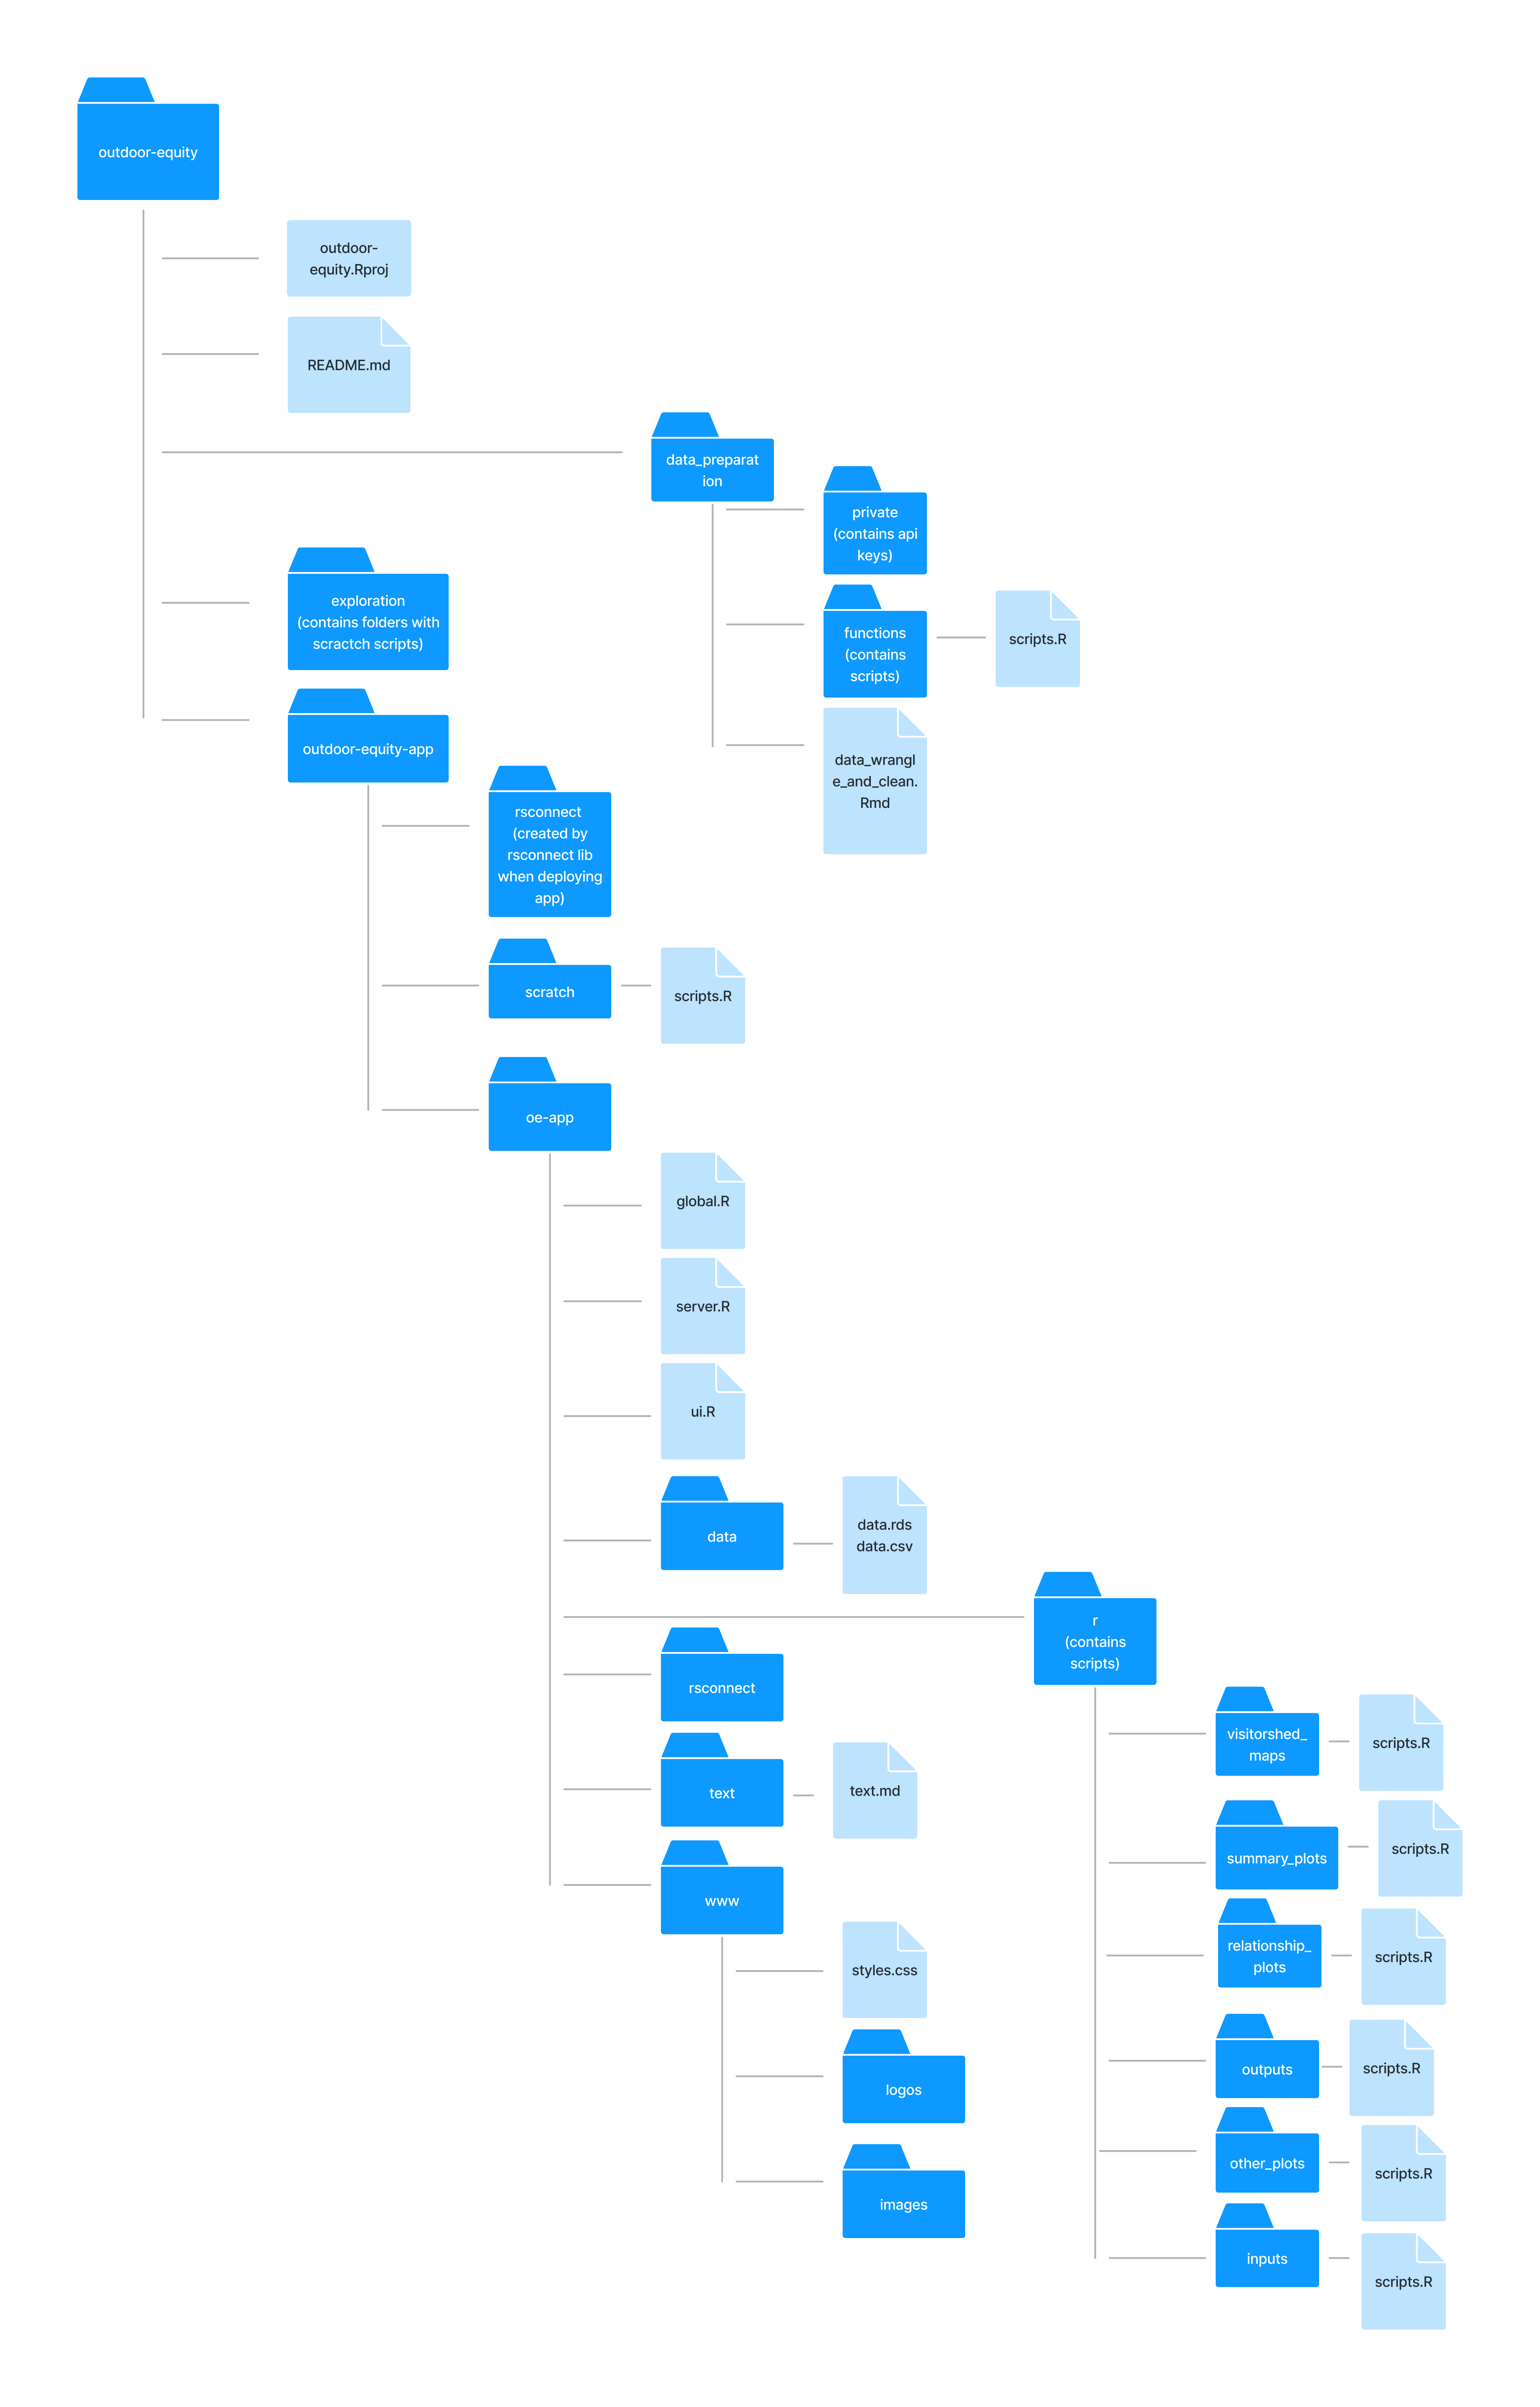
\includegraphics[width=18.73in]{images/repo_directory_medfont} \caption{Screenshot of the Metadata page of the Outdoor Equity App}\label{fig:repo-directory}
\end{figure}

  \bibliography{book.bib,packages.bib}

\end{document}
